\documentclass{article}
\usepackage{amsmath,amsfonts,amsthm,amssymb,chemformula,float,fullpage,graphicx,multicol,multirow,parskip,setspace,tikz,xcolor}
\usepackage[backend=biber,sorting=none,style=numeric-comp,giveninits]{biblatex}
\usepackage[colorlinks=true,citecolor=blue,linkcolor=black,urlcolor=blue]{hyperref}
\usetikzlibrary{matrix, fit}

\DeclareNameAlias{default}{family-given}
\renewbibmacro{in:}{}
\addbibresource{references.bib}

\DeclareMathOperator{\Gal}{Gal}
\DeclareMathOperator{\tr}{tr}

\newtheorem{proposition}{Proposition}

\onehalfspacing

\begin{document}
    \thispagestyle{empty}
    
    \begin{center}
        {\huge Cyclotomic Structure and Galois Actions\\\vspace{0.25em}of Molecular Symmetry Point Groups}\vspace{1cm}
        
        {\large Margaret A. Barker\\Advisor: Dr. Lilit Martirosyan\vspace{1cm}
        
        University of North Carolina Wilmington\\Department of Mathematics and Statistics\vspace{1cm}
        
        \today}
    \end{center}

    \vfill

    \section*{Abstract}

    We explore the algebraic and number-theoretic structure underlying molecular symmetry through the lens of representation theory. We begin by introducing molecular point groups and their matrix representations, focusing on concrete examples of the point groups $C_{2v}$ and $C_{3v}$, which describe the symmetries of water and ammonia molecules, respectively. Then, we construct character tables and decompose the representations into irreducible components. We illustrate how symmetry-adapted linear combinations (SALCs) provide a natural basis for this decomposition.

Building on this representation-theoretic framework, we analyze the eigenvalues and minimal polynomials of symmetry operations. We show that these eigenvalues are roots of unity and hence lie in cyclotomic fields. We also show that for a symmetry operation of order $n$, the minimal polynomial over $\mathbb{Q}$ divides $x^n-1$, hence it factors as a product of cyclotomic polynomials. Motivated by the observation that some character tables contain only integer values despite arising from cyclotomic fields, we investigate the role of Galois automorphisms in governing the structure of character values.

Finally, we extend this analysis to point groups exhibiting fivefold symmetry, where non-integer character values arise. In these cases, we demonstrate that for certain point groups, Galois symmetry shows that relevant character values lie in the real subfield $\mathbb{Q}(\sqrt5)\subset\mathbb{Q}(\zeta_5)$, revealing a deeper connection between molecular symmetry and algebraic number theory. Our central result is that the structure of character tables for molecular point groups is governed by cyclotomic fields and their associated Galois groups.

    \pagebreak

    \tableofcontents

    \pagebreak

    \section{Introduction}

    Symmetry is a bridge that connects the world that we can see with the quantum mechanical realm that governs the laws of chemistry. The language that describes symmetry is that of algebra. Countless chemical processes are connected to the symmetry of molecules, and a deep understanding of these concepts is rooted in group theory, representation theory, and character theory.

    This paper has three main goals. The first goal is to introduce the notation of molecular point groups often encountered in chemistry, and how to categorize molecules as belonging to a point group using a set of rules. The second goal is to describe the mathematical derivation of character tables, which are essentially a formulation of the group-theoretic structure of symmetry groups into an easy-to-understand table. Character tables are derived directly from matrix representations for the point groups $C_{2v}$ and $C_{3v}$, chosen since they describe the ubiquitous molecules, water (\ch{H2O}) and ammonia (\ch{NH3}), respectively. We use the character tables to decompose the matrix representations into irreducible representations. The third goal is to analyze the character table entries from a number-theoretic point of view. To achieve this goal, we first look at the eigenvalues and minimal polynomials of those matrices. We will see that the eigenvalues lie in cyclotomic fields and that the minimal polynomials factor into cyclotomic polynomials.

    From these observations for the specific point groups $C_{2v}$ and $C_{3v}$, we then formulate and prove some propositions that show that these characterizations hold in general. We will see that eigenvalues of symmetry operations are roots of unity, so that the characters lie in cyclotomic fields such as $\mathbb{Q}(\zeta_n)$. This goes a long way towards understanding the number-theoretic basis of the character tables, but it leaves some questions unanswered. For example, even though the characters of $C_{3v}$ lie in the cyclotomic field $\mathbb{Q}(\zeta_3)$, the characters of $C_{3v}$ are all integers. To gain understanding of why that is the case, we then pivot to Galois theory. We look at the behavior of primitive $n$th roots of unity and eigenvalues under Galois automorphisms, which will help explain why the characters of $C_{3v}$ lie in $\mathbb{Z}$.

    However, as we will see, there exist character tables that apply to actual molecules that do not have integer characters. In particular, some molecules with fivefold symmetries, such as corannulene and ferrocene, belong to point groups whose character values involve the golden ratio, and we will see that under the same Galois automorphisms, the relevant Galois-invariant character values lie in $\mathbb{Q}(\sqrt{5})$ rather than in $\mathbb{Q}(\zeta_5)$ or $\mathbb{Q}$.

    The central idea of this paper is that the eigenvalues of symmetry operations lie in cyclotomic fields, and the action of the corresponding Galois groups explains the algebraic structure of the character values appearing in molecular point group representations.
    
    Much of the presentation of point groups and character theory, up until the discussion of minimal polynomials and eigenvalues, follows the treatments in \cite{miessler2014,mcgrady2024,vallance,young}.
    
    \section{Molecular point groups}

    Many molecules contain \emph{symmetry elements}, such as rotational axes, mirror planes, and inversion centers, upon which \emph{symmetry operations} can be performed, such as rotation, reflection, or inversion. A molecule is indistinguishable before and after any symmetry operation it possesses.

    The most basic symmetry operation is $E$, the identity operation. This is the act of doing nothing, and is required in order to express a collection of symmetries as a group.

    Let $n\geq2$ be an integer. A proper rotation, $C_n$, is a rotation that can be achieved in three-dimensional space. It is a rotation through $360^\circ/n$ counterclockwise with respect to some axis.\footnote{Angles in chemistry are typically expressed in degrees, so we will use that convention throughout this paper.} We have that $C_n^n\equiv E$, so that the order of the rotation $C_n$ is $n$. If a molecule has more than one rotational axis, the one of highest order is called the \emph{principal axis}. By convention, a $C_2$ axis will be denoted $C_2'$ if it passes \emph{through} outer atoms, and $C_2''$ if it passes \emph{between} outer atoms.

    A reflection over a mirror plane is denoted $\sigma$. In particular, a reflection plane that is perpendicular to the principal axis is called horizontal and denoted $\sigma_h$. A reflection plane that includes the principal axis is called vertical and denoted $\sigma_v$. A vertical reflection plane that bisects the angle between two $C_2$ axes is called dihedral and denoted $\sigma_d$.

    The inversion operation, $i$, is where every point of the molecule is moved through the inversion center (the center of the molecule) to its opposite position the same distance from the center.

    An improper rotation, $S_n$, also called a rotation-reflection, is a $C_n$ rotation followed by a $\sigma_h$ reflection through a plane perpendicular to the rotation axis. An $S_2$ operation is equivalent to an inversion $i$. In some molecules, $S_j$ axes are coincident with $C_k$ axes, where $j$ and $k$ may or may not be equal depending on the specific molecule.

    The collection of symmetry operations that a molecule possesses determines its \emph{point group}. It is named such since at least one point in space is invariant under each symmetry operation, and the symmetry elements and operations have a group structure. This paper uses Schoenflies notation, named for Arthur Moritz Schoenflies, to denote point groups, following standard conventions in chemistry. \cite{mcgrady2024}

    \subsection{Categorization of molecules into point groups}

    There is a sequence of steps that can be followed to determine the point group of a molecule. To get started, we can classify molecules as being of \emph{low symmetry}, \emph{high symmetry}, or neither. We will list the point groups of the three categories and show example molecules that exhibit each group. To assist in determining the point groups for molecules of neither low nor high symmetry, we will use a flowchart.

    \subsubsection{Point groups of low symmetry}

    Molecules in the $C_1$ group have no symmetry besides the identity. (Indeed, every point group has the identity, but it will not be mentioned in the following groups.) An example is bromochlorofluoromethane (\ch{CHBrClF}).

    \begin{center}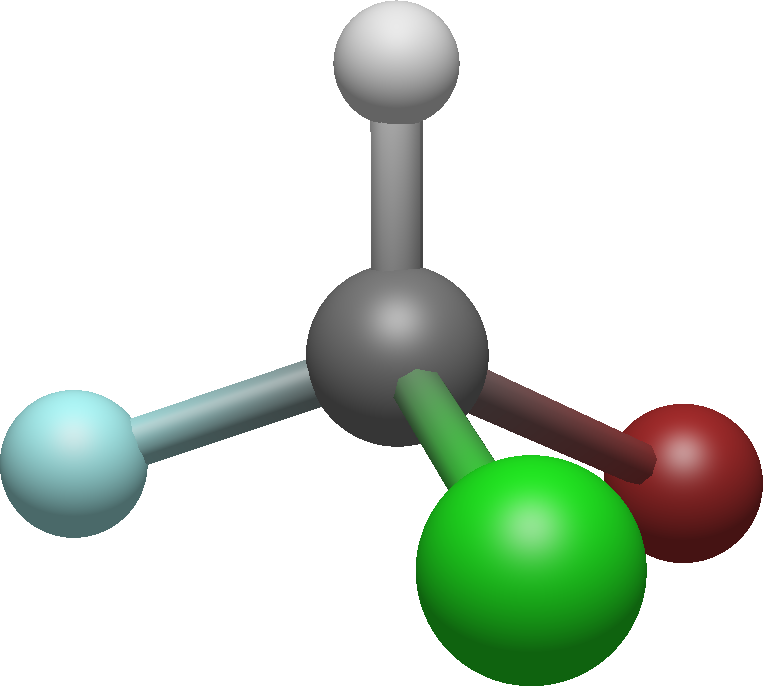
\includegraphics[width=1in]{figures/c1example.png}\end{center}

    Molecules in the $C_s$ group have only one mirror plane (in the following example, the mirror plane is the plane of the molecule). An example is 1-bromo-1-chloroethene (\ch{C2H2BrCl}).

    \begin{center}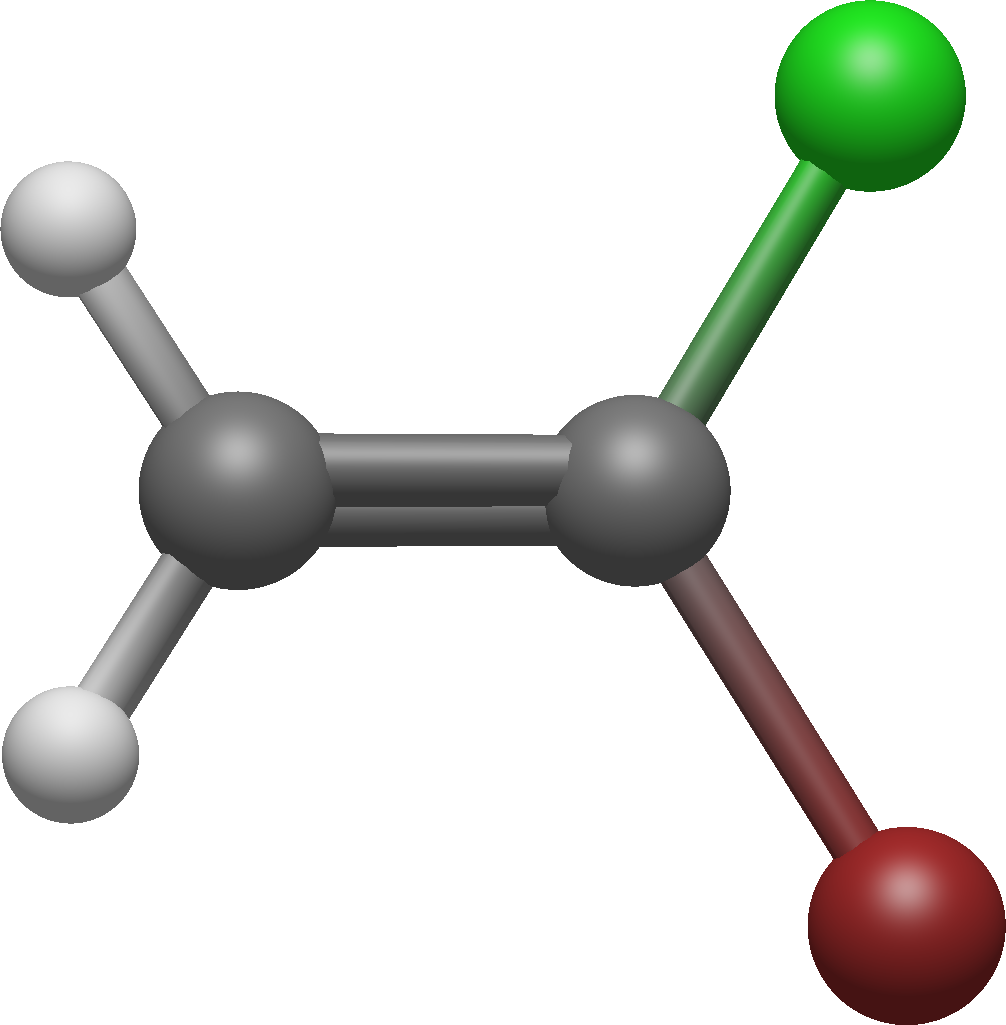
\includegraphics[width=1in]{figures/csexample.png}\end{center}

    Molecules in the $C_i$ group have only an inversion center. An example is 1,2-dibromo-1,2-dichloroethane (\ch{C2H2Br2Cl2}).

    \begin{center}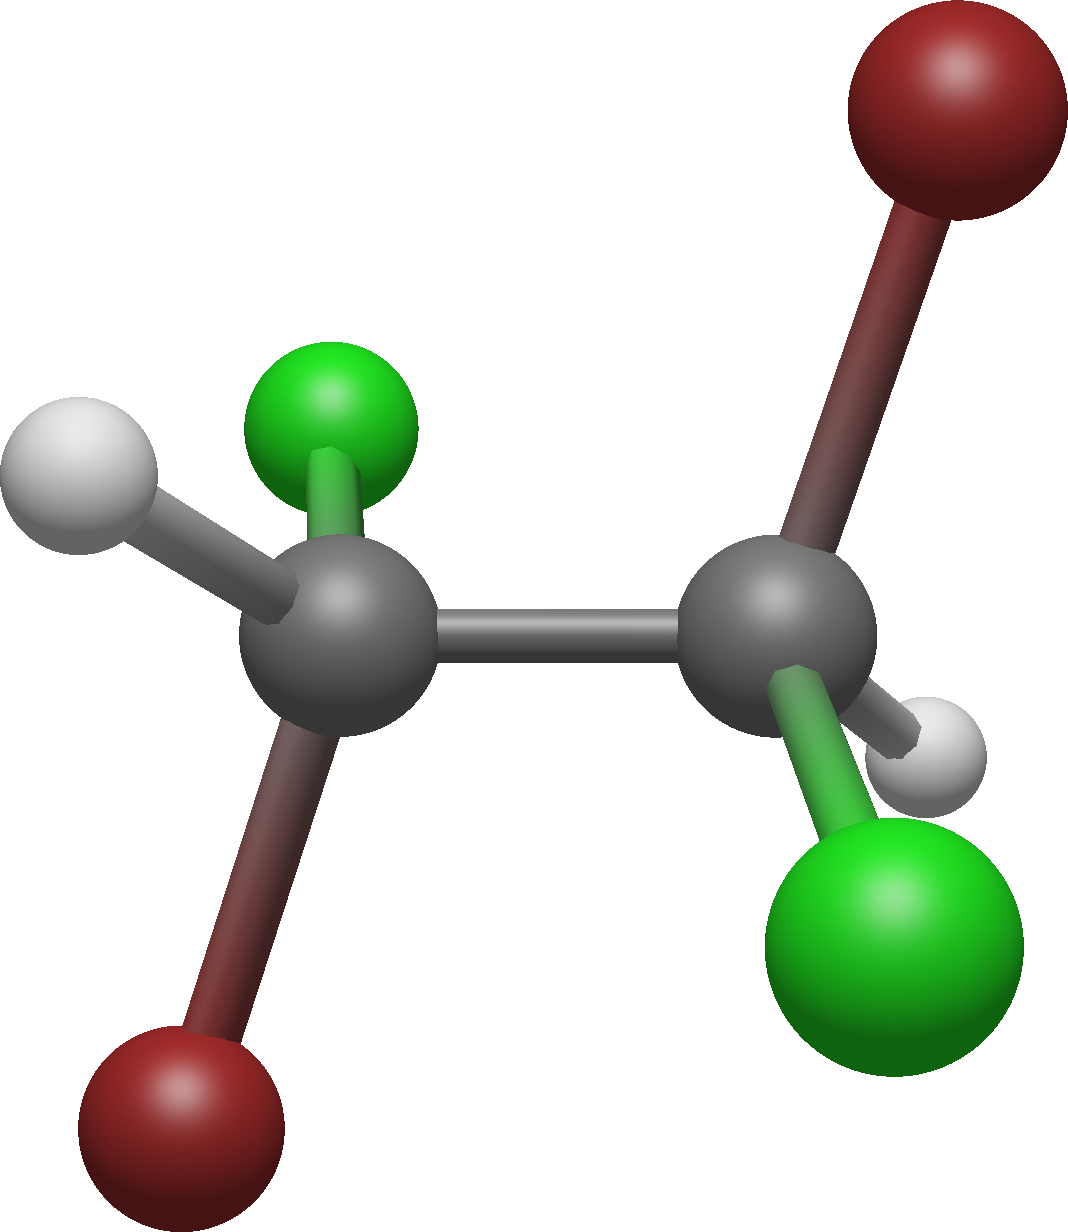
\includegraphics[width=1in]{figures/ciexample.png}\end{center}

    \subsubsection{Point groups of high symmetry}

    \label{sec:bucky}

    Molecules in the $C_{\infty v}$ group are linear, with infinite rotation order and an infinite number of reflection planes containing the rotation axis. They contain no inversion center. An example is hydrogen chloride (\ch{HCl}).

    \begin{center}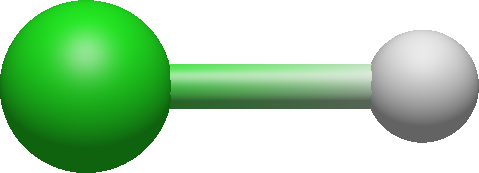
\includegraphics[width=1in]{figures/cinfvexample.png}\end{center}

    Molecules in the $D_{\infty h}$ group are like $C_{\infty v}$, but with perpendicular $C_2$ axes, a perpendicular mirror plane, and an inversion center. An example is carbon dioxide (\ch{CO2}).

    \begin{center}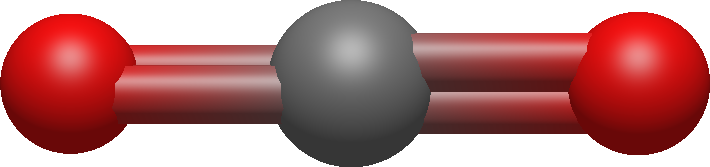
\includegraphics[width=1in]{figures/dinfhexample.png}\end{center}

    Molecules in the $T_d$ group are tetrahedral, with four $C_3$ axes, three $C_2$ axes, three $S_4$ axes, and six $\sigma_d$ mirror planes. An example is methane (\ch{CH4}).

    \begin{center}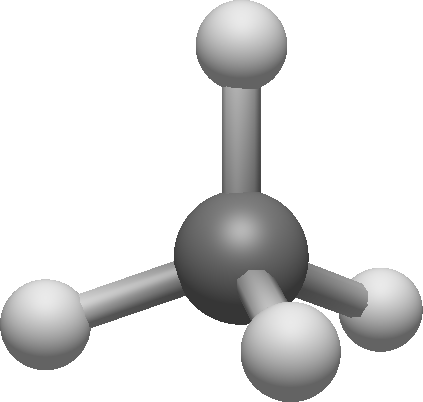
\includegraphics[width=1in]{figures/tdexample.png}\end{center}

    \enlargethispage{2\baselineskip}

    Molecules in the $O_h$ group are octahedral, with 48 symmetry operations in all. An example is sulfur hexafluoride (\ch{SF6}).

    \begin{center}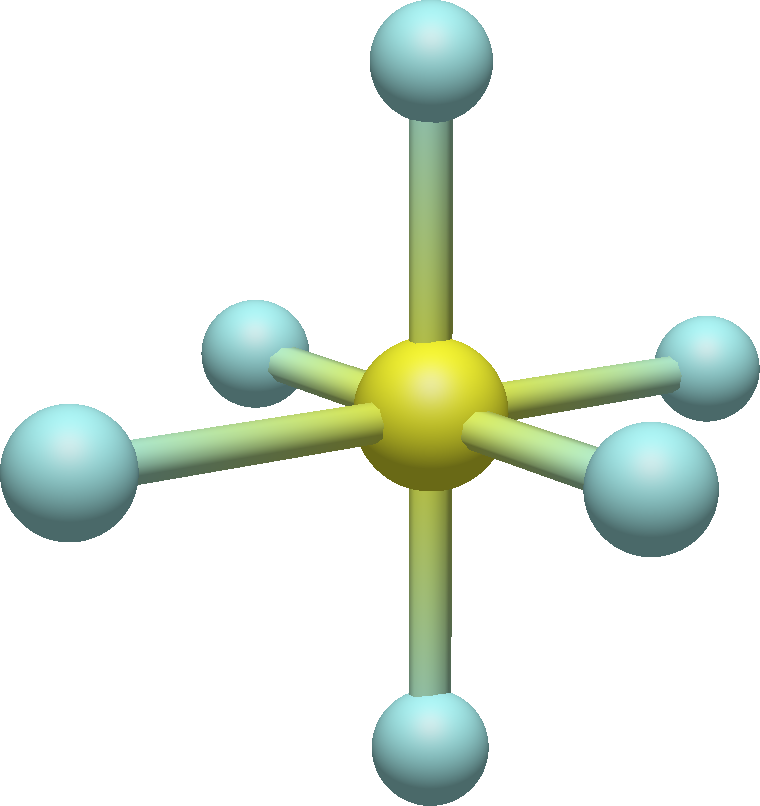
\includegraphics[width=1in]{figures/ohexample.png}\end{center}

    Molecules in the $I_h$ group are icosahedral, with 120 symmetry operations in all. A fascinating example is buckminsterfullerene (\ch{C60}), a molecule with sixty carbon atoms in a ``soccer ball'' arrangement.
    
    \begin{center}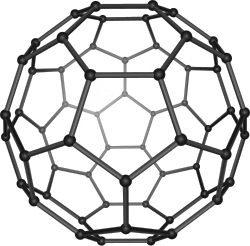
\includegraphics[width=1in]{figures/ihexample.png}\end{center}

    \subsubsection{Other point groups}

    To help distinguish which molecules are in each of the remaining point groups, we can refer to the flowchart in Figure \ref{fig:flowchart}.

    \begin{figure}[htb]
        \centering
        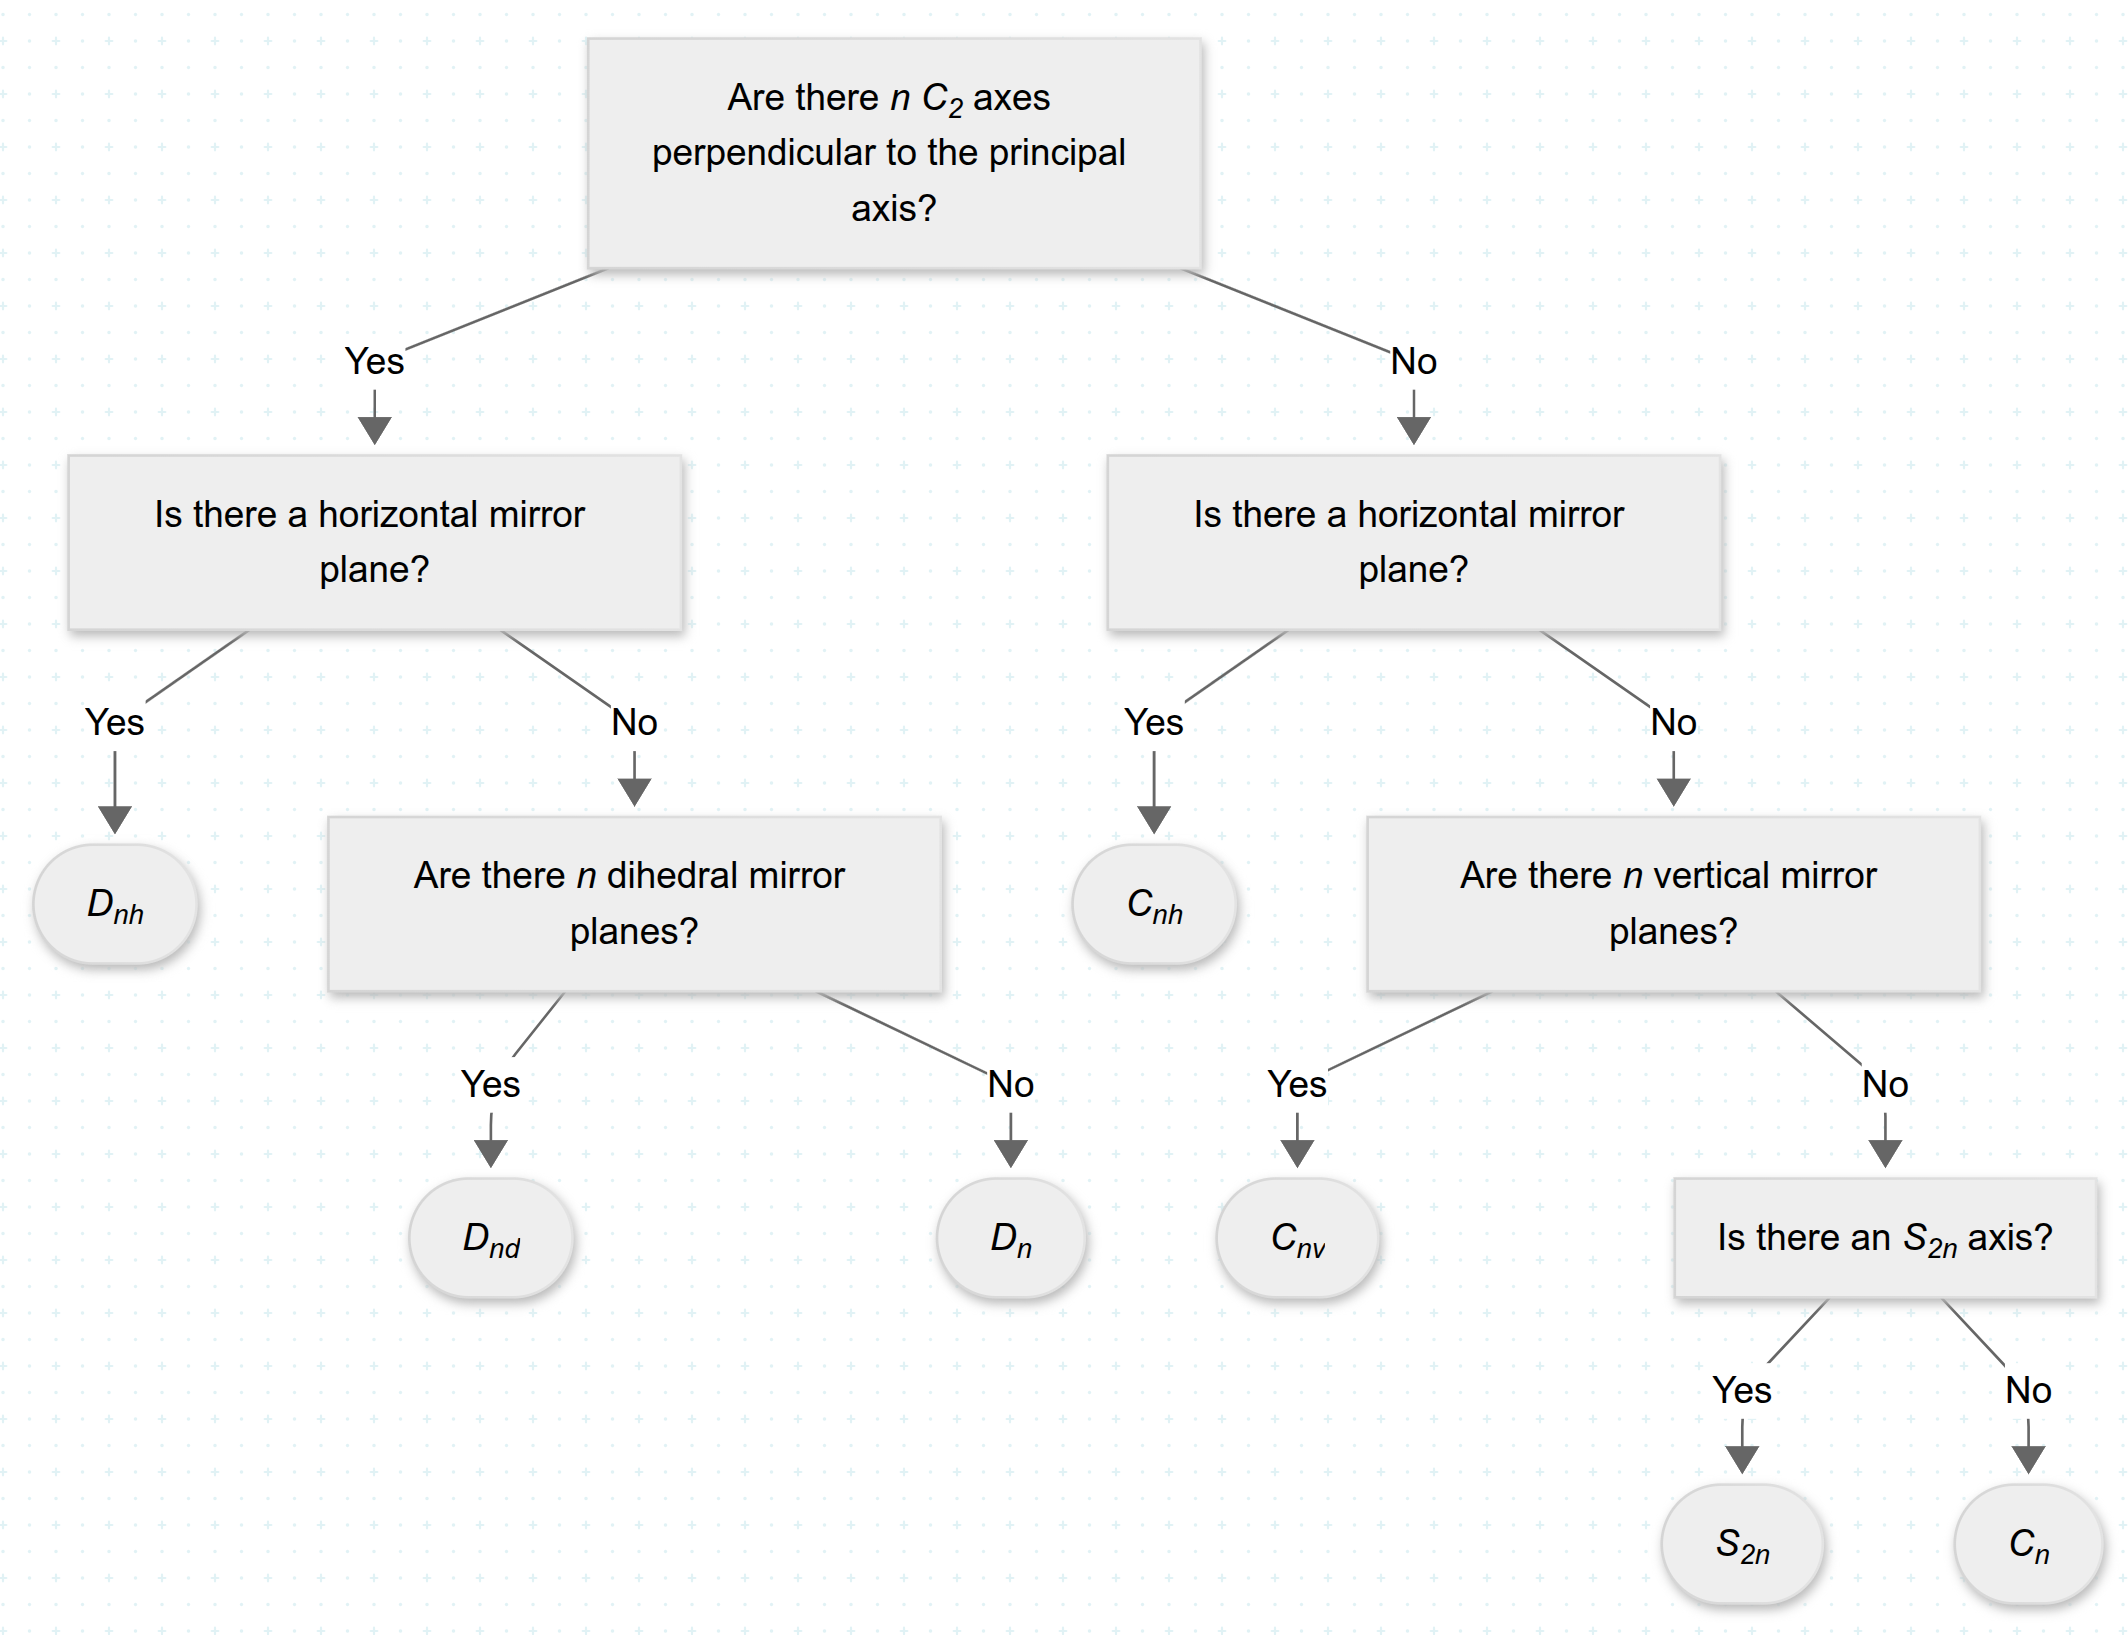
\includegraphics[width=\linewidth]{figures/flowchart.png}
        \caption{Flowchart to help determine point groups of molecules.}
        \label{fig:flowchart}
    \end{figure}

    \pagebreak

    Molecules in the $C_{nh}$ group contain a principal $C_n$ rotation axis and a horizontal mirror plane $\sigma_h$. The following examples are $C_{2h}$ (\emph{trans}-dinitrogen difluoride, \ch{N2F2}), $C_{2h}$ (1,5-dichloronaphthalene, \ch{C10H6Cl2}), and $C_{3h}$ (boric acid, \ch{H3BO3}), respectively:

    \begin{center}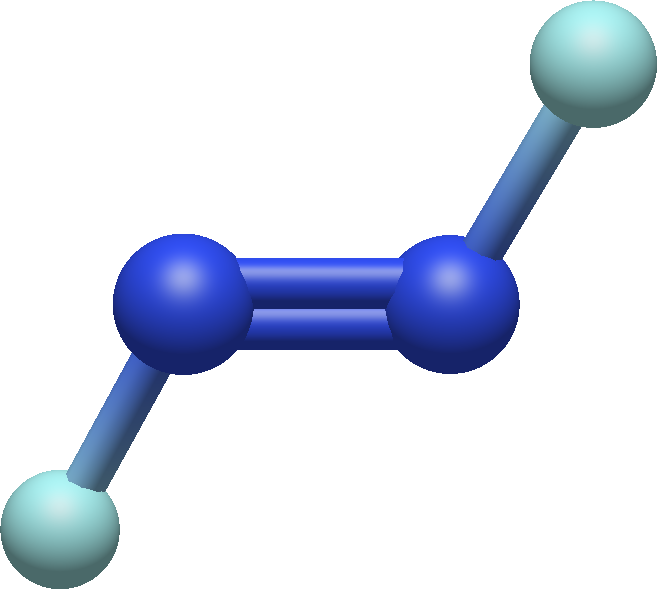
\includegraphics[width=1.2in]{figures/c2hexample1.png}\quad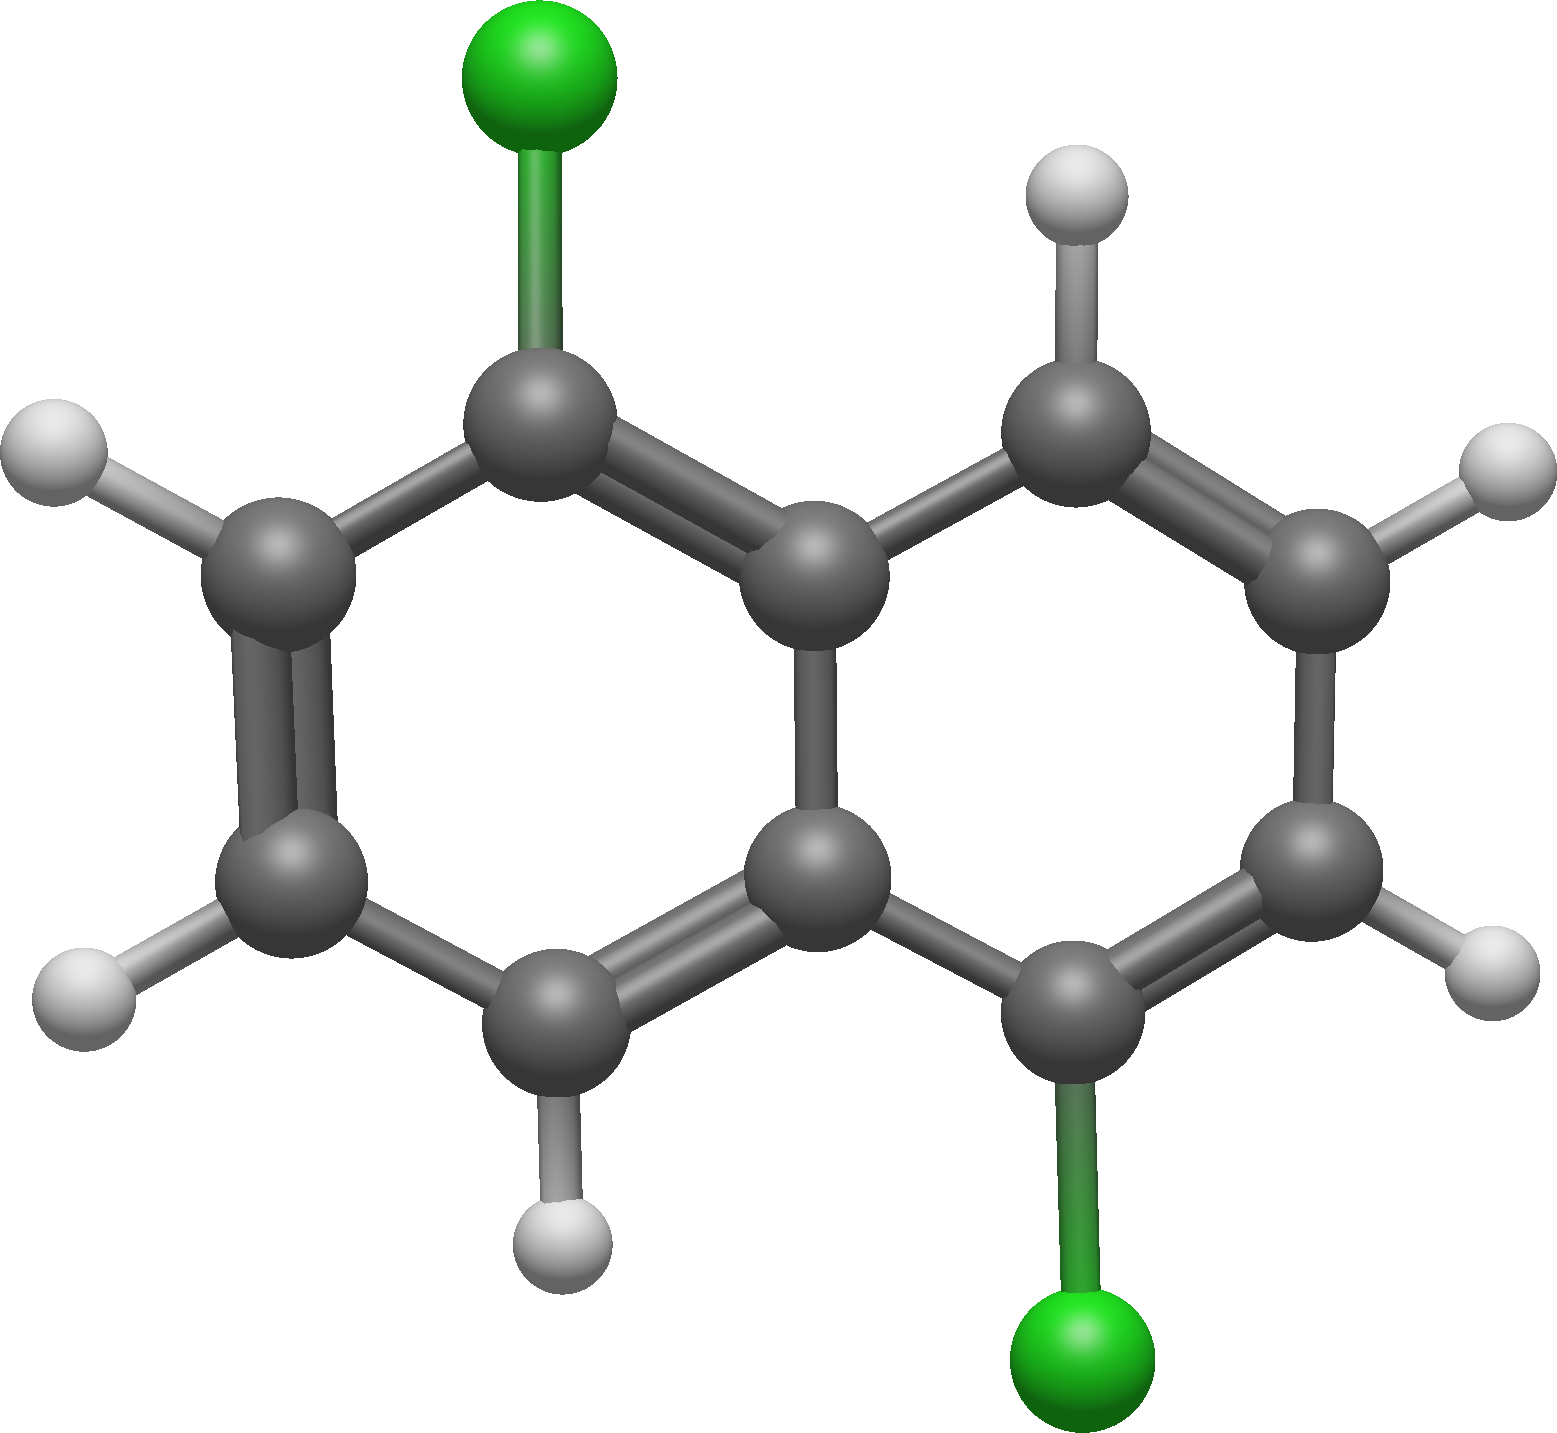
\includegraphics[width=1.2in]{figures/c2hexample2.png}\quad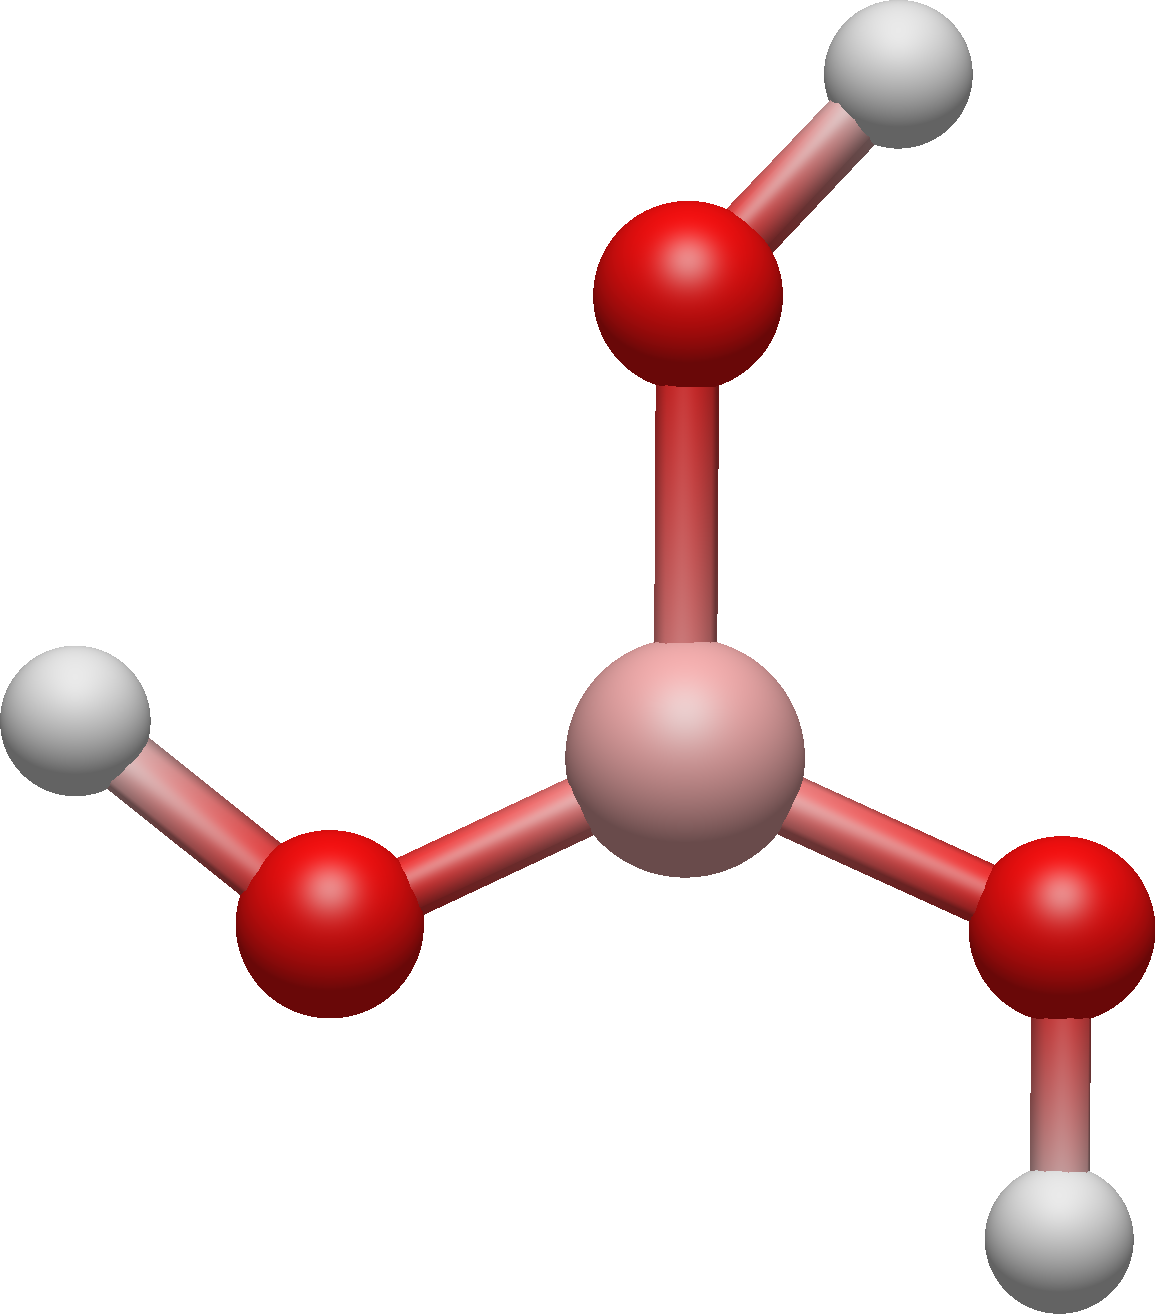
\includegraphics[width=1in]{figures/c3hexample.png}\end{center}

    Molecules in the $C_{nv}$ group contain a principal $C_n$ rotation axis and $n$ vertical mirror planes $\sigma_v$. The following examples are $C_{2v}$ (water, \ch{H2O}), $C_{3v}$ (ammonia, \ch{NH3}), and $C_{4v}$ (bromine pentafluoride, \ch{BrF5}), respectively:

    \begin{center}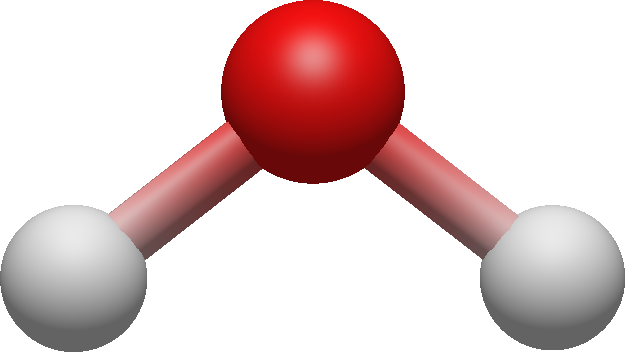
\includegraphics[width=1in]{figures/c2vexample.png}\quad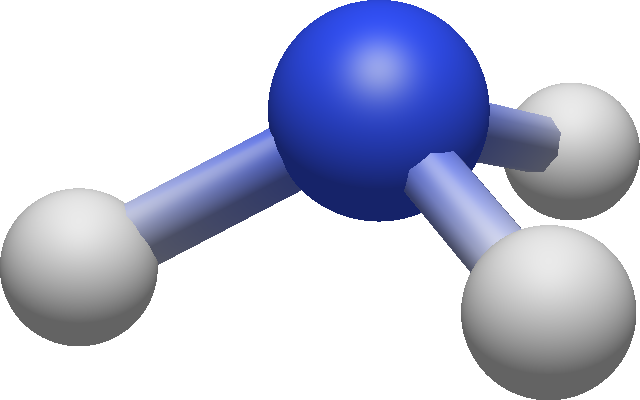
\includegraphics[width=1in]{figures/c3vexample.png}\quad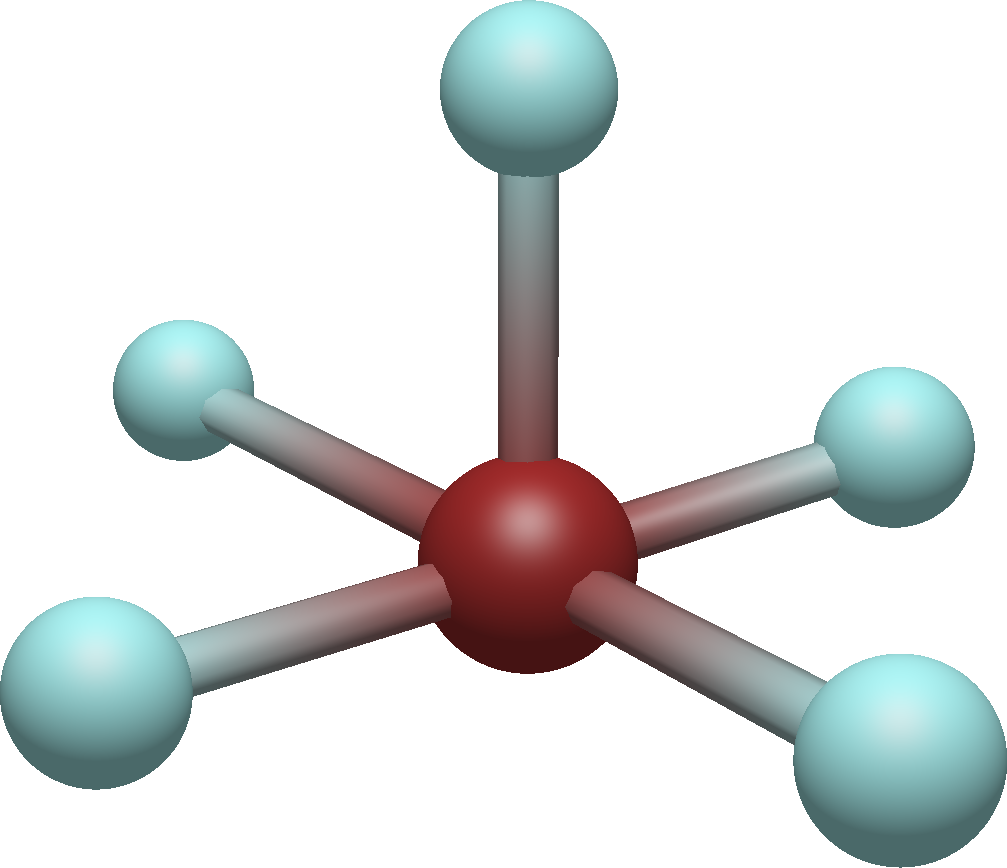
\includegraphics[width=1in]{figures/c4vexample.png}\end{center}

    Due to the importance of water and ammonia, we will devote much of our mathematical study to the point groups $C_{2v}$ and $C_{3v}$ in the following sections.

    Molecules in the $C_{n}$ group contain a principal $C_n$ rotation axis but no mirror planes. An example is hydrogen peroxide (\ch{H2O2}), which is in the point group $C_2$.

    \begin{center}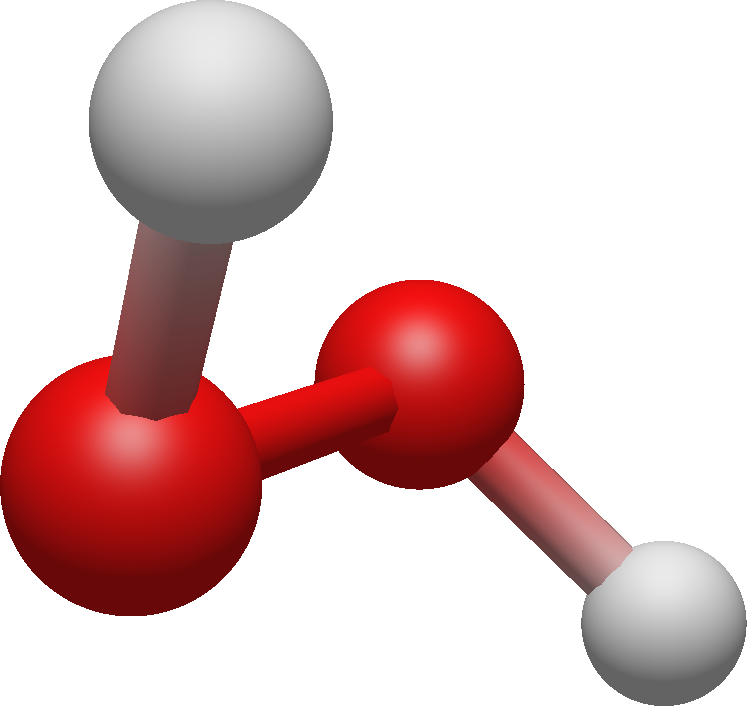
\includegraphics[width=0.9in]{figures/c2example.png}\end{center}

    Molecules in the $D_{nh}$ group contain a principal $C_n$ rotation axis and $n$ perpendicular $C_2$ rotation axes. They also have a horizontal mirror plane $\sigma_h$. The following examples are $D_{3h}$ (boron trifluoride, \ch{BF3}), $D_{3h}$ (phosphorus pentafluoride, \ch{PF5}), $D_{4h}$ (xenon tetrafluoride, \ch{XeF4}), and $D_{6h}$ (benzene, \ch{C6H6}), respectively:

    \begin{center}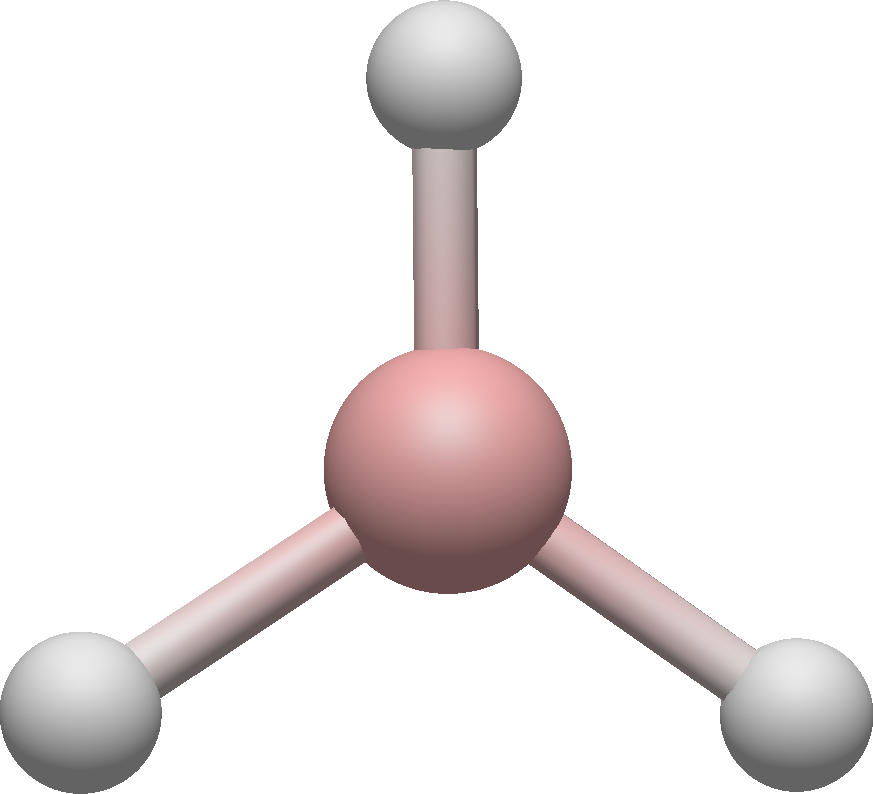
\includegraphics[width=1in]{figures/d3hexample1.png}\quad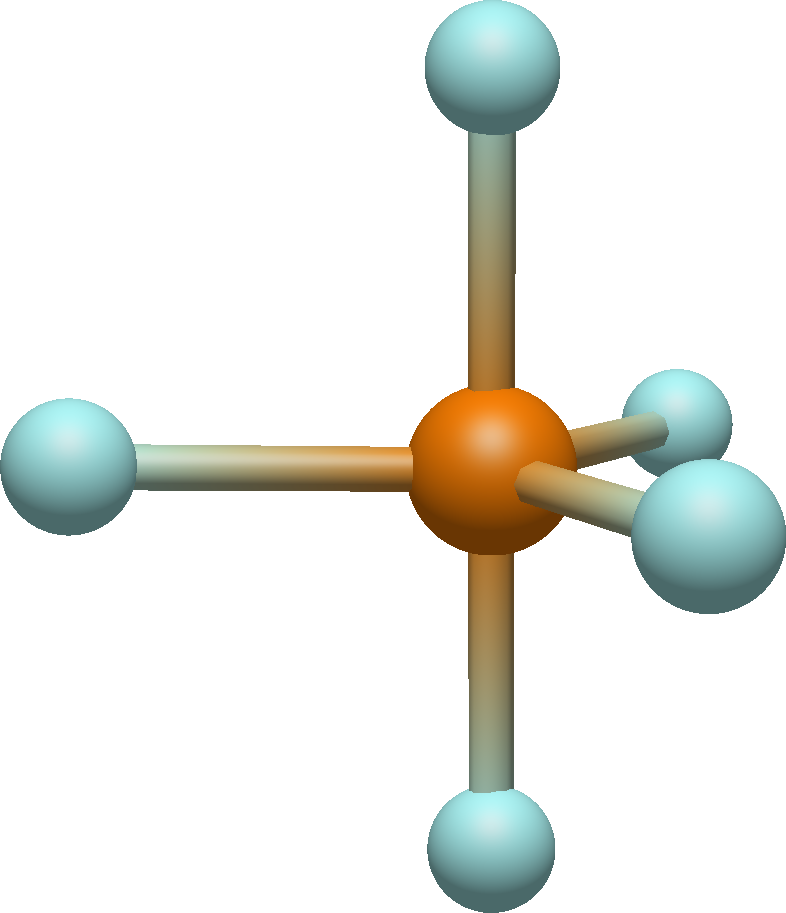
\includegraphics[width=0.8in]{figures/d3hexample2.png}\quad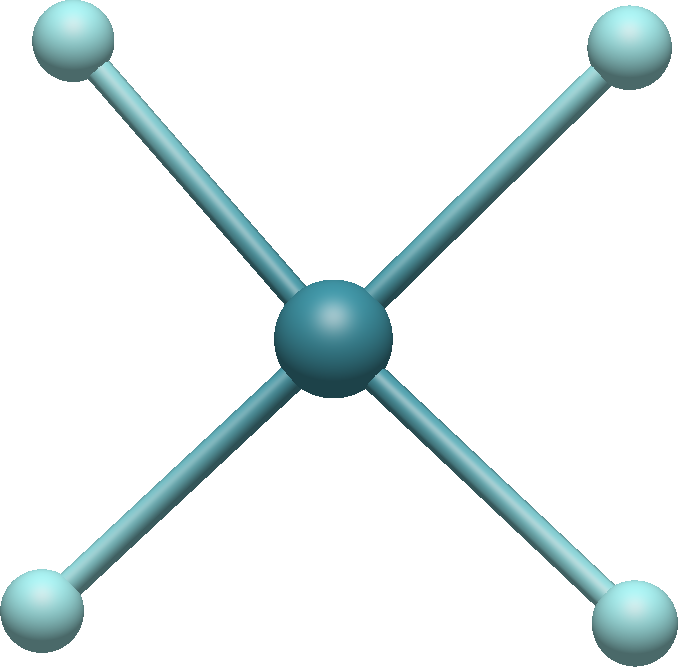
\includegraphics[width=1in]{figures/d4hexample.png}\quad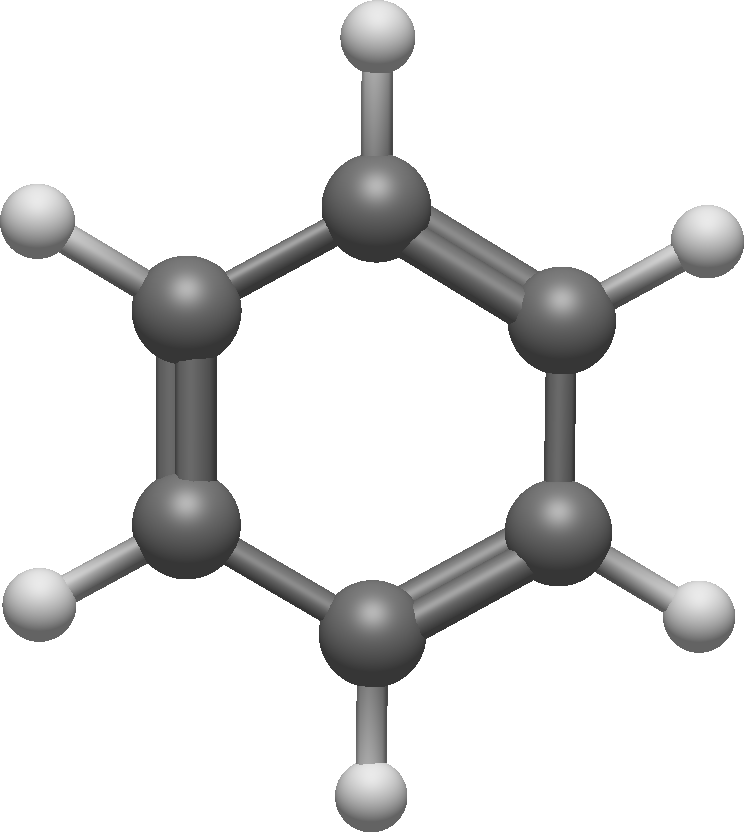
\includegraphics[width=1in]{figures/d6hexample.png}\end{center}

    \pagebreak

    Molecules in the $D_{nd}$ group contain a principal $C_n$ rotation axis and $n$ perpendicular $C_2$ rotation axes. They also have $n$ dihedral mirror planes $\sigma_d$. An example is ethane (\ch{C2H6}), which is in the point group $D_{3d}$.
    \begin{center}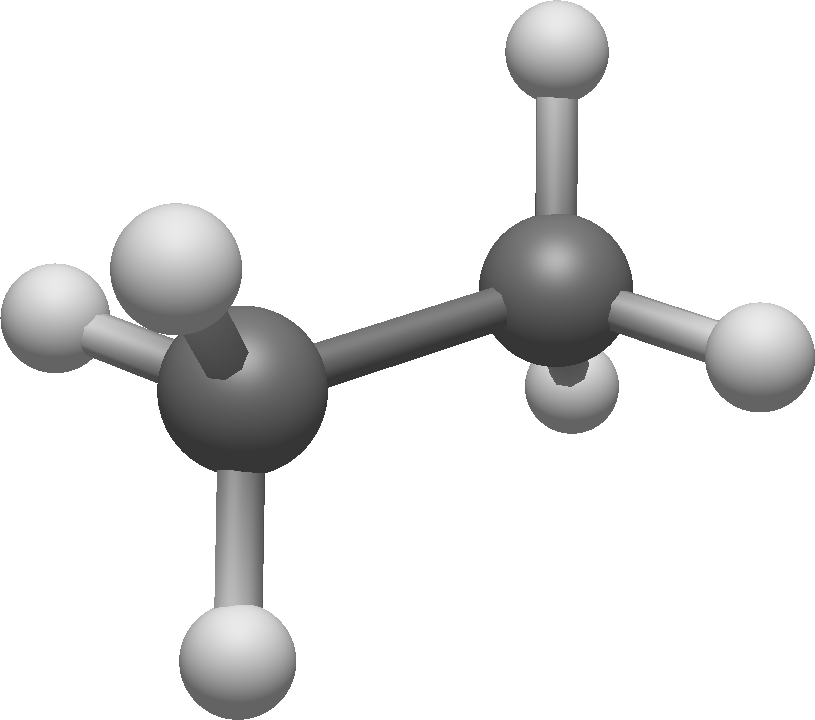
\includegraphics[width=1in]{figures/d3dexample.png}\end{center}

    Molecules in the $D_{n}$ group contain a principal $C_n$ rotation axis and $n$ perpendicular $C_2$ rotation axes, but no mirror planes. One interesting example of a $D_3$ molecule is the tris(ethylenediamine)cobalt(III) coordinate complex (\ch{[Co(en)3]^3+}, where \ch{en} = \ch{C2H8N2}). Look carefully at the geometry of the central cobalt atom (inset) and note the propeller shape.
    \begin{center}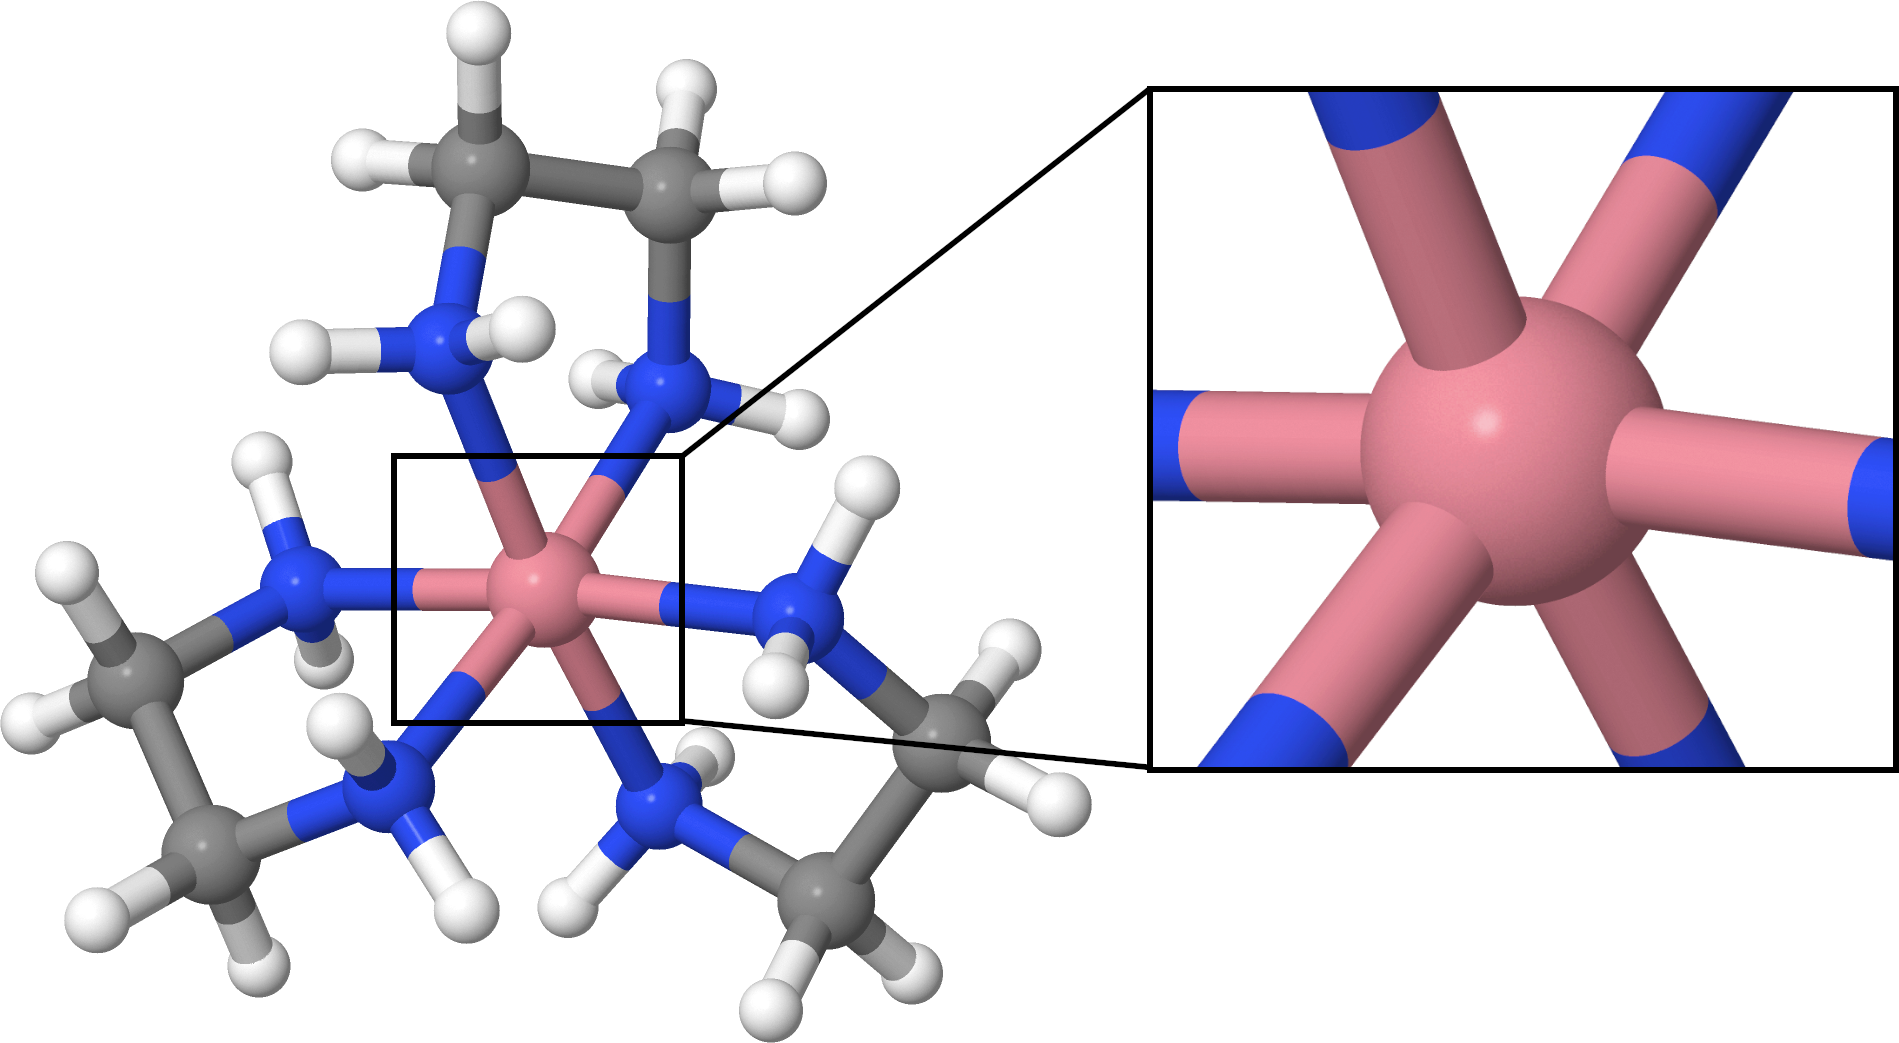
\includegraphics[width=5in]{figures/d3example.png}\end{center}

    Molecules are in the $S_{2n}$ group if they contain an $S_{2n}$ rotation-reflection axis, one principal $C_n$ rotation axis, and if they do not qualify to be in any of the $C$ or $D$ point groups. One molecule in the point group $S_4$ is 1,3,5,7-tetrafluorocyclooctatetraene (\ch{C8H4F4}), shown here from three different perspectives. Notice that the central carbon ring has an ``octagon boat'' shape.

    \begin{center}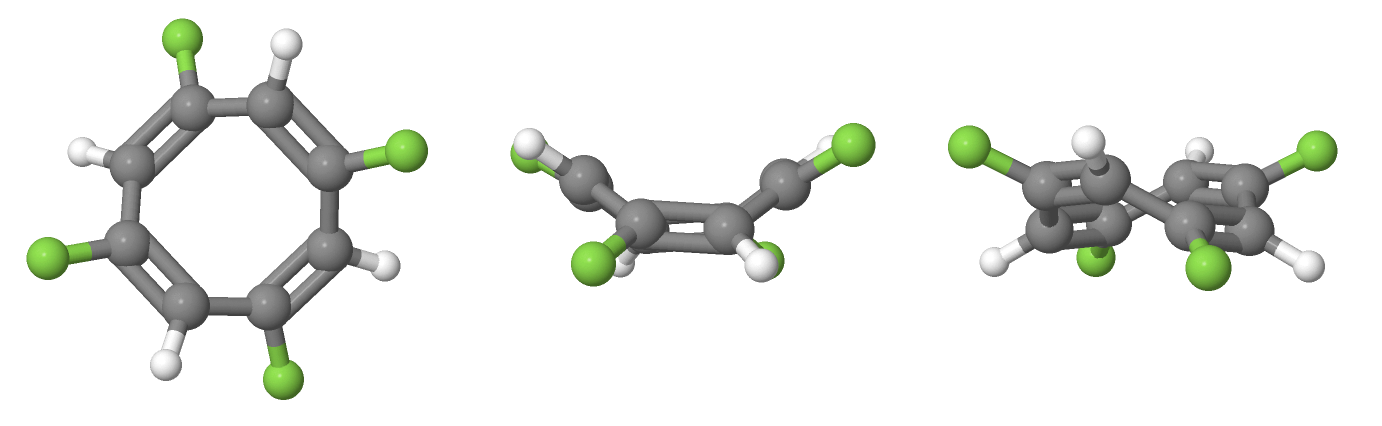
\includegraphics[width=\linewidth]{figures/s4example.png}\end{center}

    \section{Algebraic structure of the point groups \texorpdfstring{$C_{2v}$ and $C_{3v}$}{C2v and C3v}}

    To gain a deeper understanding of point groups, we need to look at them using techniques of group theory. The first thing that we need to do is to verify that point groups truly fit the algebraic definition of a group. To illustrate the group structure of the point groups, we will use the point groups of water (\ch{H2O}), $C_{2v}$, and ammonia (\ch{NH3}), $C_{3v}$, as examples.
    
    First, we will verify that $C_{2v}$ satisfies the definition of a group by showing that it has an identity, inverses, closure, and associativity. Every point group, including $C_{2v}$, has a symmetry operation $E$ which serves as the identity element of the group. The $C_2$ rotation is its own inverse, as $C_2C_2=C_2^2=E$. The reflections $\sigma_{v1}$ and $\sigma_{v2}$ are their own inverses. There are $4$ symmetry operations in $C_{2v}$: $\{E, C_2, \sigma_{v1}, \sigma_{v2}\}$. The Cayley table for $C_{2v}$ is shown in Table \ref{tab:c2vcayley}. Closure can be verified from the Cayley table, and associativity follows from the associativity of function composition. Furthermore, from the Cayley table, we can see that the point group $C_{2v}$ is isomorphic to the Klein 4-group $V_4$.

    \begin{table}[ht]
        \centering
        \renewcommand{\arraystretch}{1.5}
        \begin{tabular}{lcr}
            \begin{tabular}{l}
                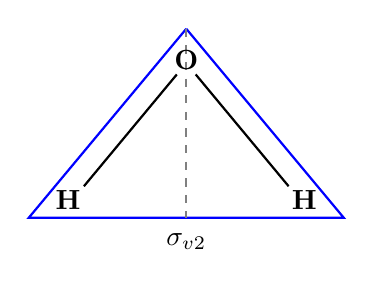
\begin{tikzpicture}[scale=2]
                    \coordinate (one) at (0,1.2);
                    \coordinate (two) at (1,0);
                    \coordinate (three) at (-1,0);
                    \coordinate (onetwo) at (0.5,0.866);
                    \coordinate (twothree) at (0,0);
                    \coordinate (onethree) at (-0.5,0.866);
                    \draw [blue,thick] (one)--(two)--(three)--(one);
                    \draw [gray,thick,dashed] (one)--(twothree);
                    \draw [black,thick,solid] (-0.06,0.91)--(-0.65,0.2);
                    \draw [black,thick,solid] (0.06,0.91)--(0.65,0.2);
                    \node at (0,-0.15) {$\sigma_{v2}$};
                    \node at (0,1) {\textbf O};
                    \node at (-0.75,0.11)
                    {\textbf H};
                    \node at (0.75,0.11)
                    {\textbf H};
                \end{tikzpicture}\\
                \begin{tabular}{l}
                    $E$: Identity\\
                    $C_2$: $180^{\circ}$\\
                    $\sigma_{v1}$: Reflection over molecular plane
                \end{tabular}
            \end{tabular}
            & \hspace{0.25in} &
            \begin{tabular}{cc|cccc}
                & & \multicolumn{4}{c}{$g$}\\
                & $f \circ g$ & $E$ & $C_2$ & $\sigma_{v1}$ & $\sigma_{v2}$\\
                \hline
                \multirow{4}{*}{$f$} & $E$ & $E$ & $C_2$ & $\sigma_{v1}$ & $\sigma_{v2}$\\
                & $C_2$ & $C_2$ & $E$ & $\sigma_{v2}$ & $\sigma_{v1}$\\
                & $\sigma_{v1}$ & $\sigma_{v1}$ & $\sigma_{v2}$ & $E$ & $C_2$\\
                & $\sigma_{v2}$ & $\sigma_{v2}$ & $\sigma_{v1}$ & $C_2$ & $E$
            \end{tabular}
        \end{tabular}
        \caption{The Cayley table for the point group $C_{2v}$, using water (\ch{H2O}) as an example.}
        \label{tab:c2vcayley}
    \end{table}
    
    We will verify that $C_{3v}$ satisfies the definition of a group in the same way as for $C_{2v}$. Clearly, $C_{3v}$ has the identity symmetry $E$. The $C_3$ rotation has the inverse $C_3^2$, as $C_3C_3^2=C_3^3=E$ and $C_3^2C_3=C_3^3=E$. Likewise, $C_3^2$ has the inverse $C_3$. Each reflection $\sigma_{v}$ is its own inverse. Note that $C_{3v}$ does not have a perpendicular $C_2$ axis or a $\sigma_h$ horizontal mirror plane (\ch{NH3} is trigonal pyramidal, not trigonal planar). We have that the point group $C_{3v}$ is isomorphic to the $S_3$ permutation group, since the symmetries of \ch{NH3} correspond to the permutations of the triangle of three hydrogen atoms. Thus there are $3!=6$ symmetry operations in $C_{3v}$: $\{E, C_3, C_3^2, \sigma_{v1}, \sigma_{v2}, \sigma_{v3}\}$. Note that $C_{3v}$ is not abelian. The Cayley table for $C_{3v}$ is shown in Table \ref{tab:c3vcayley}. Closure can be verified from the Cayley table, and associativity follows from the associativity of function composition.

    \begin{table}[ht]
        \centering
        \renewcommand{\arraystretch}{1.5}
        \begin{tabular}{lcr}
            \begin{tabular}{l}
                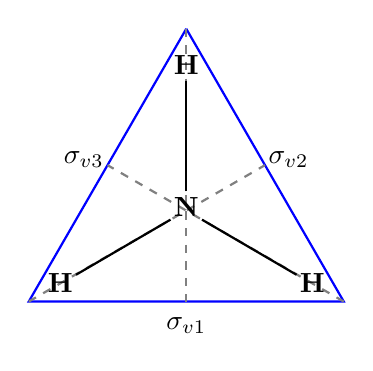
\begin{tikzpicture}[scale=2]
                    \coordinate (one) at (0,1.732);
                    \coordinate (two) at (1,0);
                    \coordinate (three) at (-1,0);
                    \coordinate (onetwo) at (0.5,0.866);
                    \coordinate (twothree) at (0,0);
                    \coordinate (onethree) at (-0.5,0.866);
                    \draw [blue,thick] (one)--(two)--(three)--(one);
                    \draw [gray,thick,dashed] (one)--(twothree);
                    \draw [gray,thick,dashed] (two)--(onethree);
                    \draw [gray,thick,dashed] (three)--(onetwo);
                    \draw [black,thick,solid] (0,0.7)--(0,1.4);
                    \draw [black,thick,solid] (-0.1,0.52)--(-0.7,0.17);
                    \draw [black,thick,solid] (0.1,0.52)--(0.7,0.17);
                    \node at (0,-0.15) {$\sigma_{v1}$};
                    \node at (0.65,0.9) {$\sigma_{v2}$};
                    \node at (-0.65,0.9)
                    {$\sigma_{v3}$};
                    \node at (0,0.6) {\textbf N};
                    \node at (0,1.5) {\textbf H};
                    \node at (-0.8,0.12) {\textbf H};
                    \node at (0.8,0.12) {\textbf H};
                \end{tikzpicture}\\
                \begin{tabular}{l}
                    $E$: Identity\\
                    $C_3$: $120^{\circ}$, counterclockwise\\
                    $C_3^2$: $240^{\circ}$, counterclockwise
                \end{tabular}
            \end{tabular}
            & \hspace{0.25in} &
            \begin{tabular}{cc|cccccc}
                & & \multicolumn{6}{c}{$g$}\\
                & $f \circ g$ & $E$ & $C_3$ & $C_3^2$ & $\sigma_{v1}$ & $\sigma_{v2}$ & $\sigma_{v3}$\\
                \hline
                \multirow{6}{*}{$f$} & $E$ & $E$ & $C_3$ & $C_3^2$ & $\sigma_{v1}$ & $\sigma_{v2}$ & $\sigma_{v3}$\\
                & $C_3$ & $C_3$ & $C_3^2$ & $E$ & $\sigma_{v3}$ & $\sigma_{v1}$ & $\sigma_{v2}$\\
                & $C_3^2$ & $C_3^2$ & $E$ & $C_3$ & $\sigma_{v2}$ & $\sigma_{v3}$ & $\sigma_{v1}$\\
                & $\sigma_{v1}$ & $\sigma_{v1}$ & $\sigma_{v2}$ & $\sigma_{v3}$ & $E$ & $C_3$ & $C_3^2$\\
                & $\sigma_{v2}$ & $\sigma_{v2}$ & $\sigma_{v3}$ & $\sigma_{v1}$ & $C_3^2$ & $E$ & $C_3$\\
                & $\sigma_{v3}$ & $\sigma_{v3}$ & $\sigma_{v1}$ & $\sigma_{v2}$ & $C_3$ & $C_3^2$ & $E$
            \end{tabular}
        \end{tabular}
        \caption{The Cayley table for the point group $C_{3v}$, using ammonia (\ch{NH3}) as an example. The viewpoint of the molecule is with the nitrogen atom in the plane of the paper and the hydrogen atoms facing away from the reader.}
        \label{tab:c3vcayley}
    \end{table}

    Now that we know molecular symmetry can be expressed in terms of algebraic groups, it is natural to consider how group theory can help us to understand observable chemical processes. To gain understanding of the underlying mathematical structure, we will use representation theory to express the symmetry operations in terms of matrices. Then we will use the principles of character theory to construct character tables, which are used by chemists to visualize the algebraic structure of various point groups in a concise and systematic way. We will use a standard system of notation to label the character tables, called \emph{Mulliken symbols}. \cite{mulliken1955}

    \section{Matrix representations of symmetry operations}

    \label{sec:matricesc2vc3v}

    \enlargethispage{\baselineskip}

    Our next step in the mathematical analysis is to find matrix representations of the symmetry operations $E$, $C_n$, $\sigma$, $i$, and $S_n$. We will define these operations as transformations of the coordinate vector $(x,y,z)^T$ in the standard Cartesian representation acting on $\mathbb{R}^3$. We place the origin at the center of symmetry. The identity operation $E$ is represented by the identity matrix \[M_E=\begin{bmatrix}1&0&0\\0&1&0\\0&0&1\end{bmatrix}.\] The rotation operation $C_n$, where the rotation is about the $z$ axis, is represented by the matrix \[M_{C_n}=\begin{bmatrix}\cos\theta&-\sin\theta&0\\\sin\theta&\cos\theta&0\\0&0&1\end{bmatrix},\] where $\theta=360^\circ/n$. Matrices for other rotational axes can be constructed similarly. The reflection operations $\sigma$ over the $xy$, $yz$, and $xz$ planes are represented by the respective matrices \[M_{\sigma_{xy}}=\begin{bmatrix}1&0&0\\0&1&0\\0&0&-1\end{bmatrix}, M_{\sigma_{yz}}=\begin{bmatrix}-1&0&0\\0&1&0\\0&0&1\end{bmatrix}, \text{ and }M_{\sigma_{xz}}=\begin{bmatrix}1&0&0\\0&-1&0\\0&0&1\end{bmatrix}.\] The inversion operation $i$ is represented by the matrix \[M_i=\begin{bmatrix}-1&0&0\\0&-1&0\\0&0&-1\end{bmatrix}.\] Finally, the rotation-reflection operation $S_n$, where the rotation is about the $z$ axis and the reflection is over the $xy$ plane, is represented by the matrix \[M_{S_n}=\begin{bmatrix}\cos\theta&-\sin\theta&0\\\sin\theta&\cos\theta&0\\0&0&-1\end{bmatrix},\] where $\theta=360^\circ/n$. Matrices for other rotational axes and reflection planes can be constructed similarly.

    Define $\mathcal B_{xyz} = (x,y,z)$ to be the standard ordered basis of $\mathbb{R}^3$.

    Now that we have a set of matrices for the symmetry operations, we can express the matrix representation of each of the point groups. To simplify the discussion, we will limit ourselves to the point groups $C_{2v}$ and $C_{3v}$. We will look at the matrix representation for $C_{2v}$ (water, \ch{H2O}) first. These matrices will be with respect to the basis $\mathcal B_{xyz}$. We use the notation established in Table \ref{tab:c2vcayley}. By convention, we set the $z$ axis as the principal axis and the $xz$ plane as the plane of the molecule, with the oxygen atom at the origin, as shown\footnote{The choice of axes is arbitrary. Mulliken recommended using $yz$ as the molecular plane for $C_{2v}$. \cite{mulliken1955} However, in this paper, we are using the convention used in Miessler, Fischer, and Tarr \cite{miessler2014}.}:
    
    \begin{center}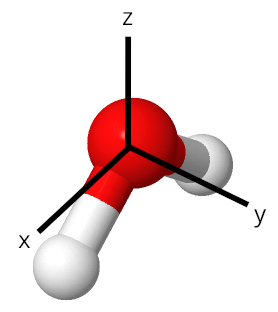
\includegraphics[width=1.25in]{figures/waterxyz.png}\end{center}
    
    Then the matrices for the symmetry operations of $C_{2v}$ are \[M_E=\begin{bmatrix}1&0&0\\0&1&0\\0&0&1\end{bmatrix}, M_{C_2}=\begin{bmatrix}-1&0&0\\0&-1&0\\0&0&1\end{bmatrix}, M_{\sigma_{v1}}=\begin{bmatrix}1&0&0\\0&-1&0\\0&0&1\end{bmatrix}, \text{ and } M_{\sigma_{v2}}=\begin{bmatrix}-1&0&0\\0&1&0\\0&0&1\end{bmatrix}.\] Multiplying these matrices reveals the same group structure as shown in Table \ref{tab:c2vcayley}.
    
    Now we will look at the matrix representation for $C_{3v}$ (ammonia, \ch{NH3}). These matrices will be with respect to the basis $\mathcal B_{xyz}$. We use the notation established in Table \ref{tab:c3vcayley}. By convention, we set the $z$ axis as the principal axis, the $xy$ plane as parallel to the hydrogen triangle, and the $xz$ plane coinciding with one of the three $\sigma_v$ mirror planes, with the nitrogen atom at the origin, as shown:
    
    \begin{center}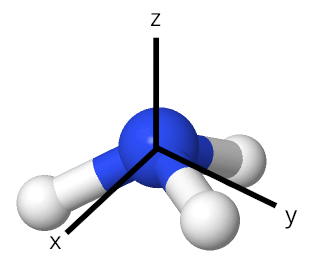
\includegraphics[width=1.5in]{figures/ammoniaxyz.png}\end{center}
    
    Then the matrices for the symmetry operations of $C_{3v}$ are \[M_E=\begin{bmatrix}1&0&0\\0&1&0\\0&0&1\end{bmatrix}, M_{C_3}=\begin{bmatrix}-\frac12&-\frac{\sqrt{3}}2&0\\\frac{\sqrt{3}}2&-\frac12&0\\0&0&1\end{bmatrix}, M_{C_3^2}=\begin{bmatrix}-\frac12&\frac{\sqrt{3}}2&0\\-\frac{\sqrt{3}}2&-\frac12&0\\0&0&1\end{bmatrix},\]
    \[M_{\sigma_{v1}}=\begin{bmatrix}1&0&0\\0&-1&0\\0&0&1\end{bmatrix}, M_{\sigma_{v2}}=\begin{bmatrix}-\frac12&-\frac{\sqrt{3}}2&0\\-\frac{\sqrt3}2&\frac12&0\\0&0&1\end{bmatrix}, \text{ and } M_{\sigma_{v3}}=\begin{bmatrix}-\frac12&\frac{\sqrt{3}}2&0\\\frac{\sqrt3}2&\frac12&0\\0&0&1\end{bmatrix}.\] Multiplying these matrices reveals the same group structure as shown in Table \ref{tab:c3vcayley}.

    \subsection{Alternative bases and construction of SALCs}

    \label{sec:salcs}

    Notice that the preceding choice of axes follows chemistry convention, but it is ultimately arbitrary. We could equally well position the molecule in the Euclidean space $\mathbb{R}^3$ in some other way. In particular, there is no intrinsic reason to use the basis $\mathcal B_{xyz}$; any basis of $\mathbb{R}^3$ may be used. For instance, for the ammonia molecule (\ch{NH3}), a natural alternative basis is given by the positions of the hydrogen atoms. To define this basis, we first fix a labeling of the hydrogen atoms $H_1, H_2, H_3$, as shown:

    \begin{center}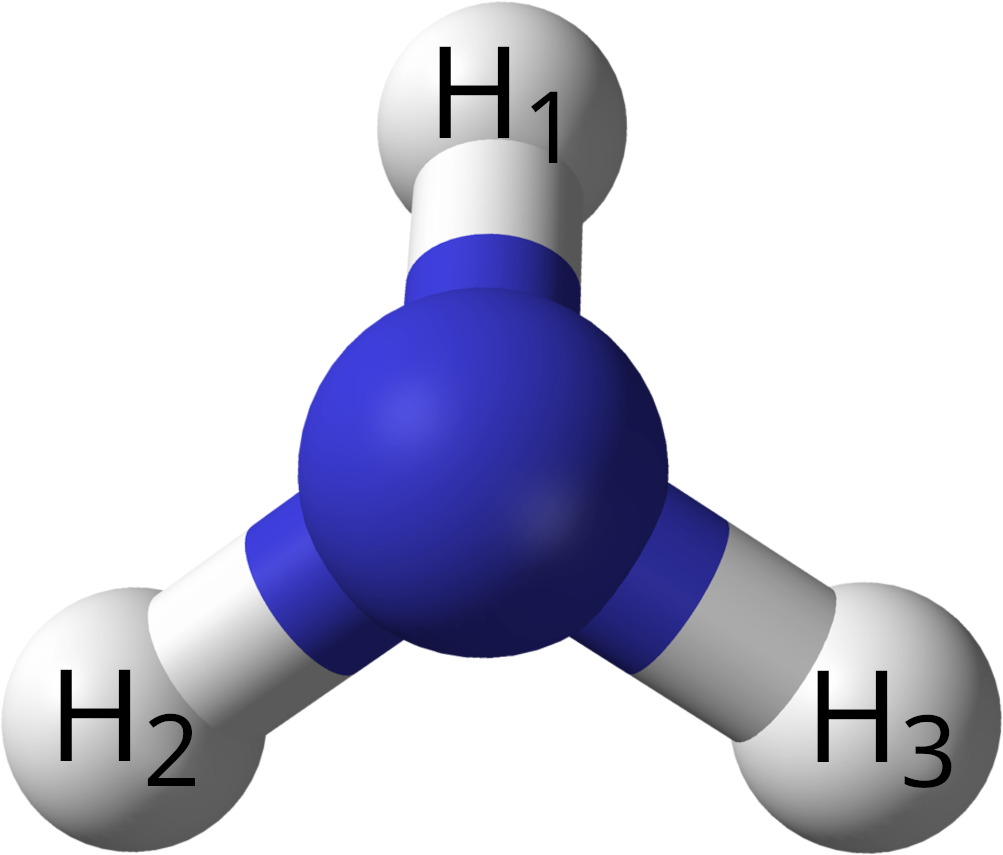
\includegraphics[width=1.25in]{figures/ammoniah1h2h3.png}\end{center}

    We define $H_1$, $H_2$, and $H_3$ to be vectors representing the positions of the hydrogen atoms relative to the central nitrogen atom, normalized to be unit length. Since ammonia is a trigonal pyramidal molecule, the nitrogen atom is not coplanar with the hydrogen atoms, so the vectors $H_1, H_2, H_3$ are linearly independent. Define the ordered basis $\beta =(H_1,H_2,H_3)$ of $\mathbb{R}^3$. The matrices with respect to $\beta$ for the symmetry operations of $C_{3v}$ are given by\[[M_E]_\beta=\begin{bmatrix}1&0&0\\0&1&0\\0&0&1\end{bmatrix}, [M_{C_3}]_\beta=\begin{bmatrix}0&0&1\\1&0&0\\0&1&0\end{bmatrix}, [M_{C_3^2}]_\beta=\begin{bmatrix}0&1&0\\0&0&1\\1&0&0\end{bmatrix},\]
    \[[M_{\sigma_{v1}}]_\beta=\begin{bmatrix}1&0&0\\0&0&1\\0&1&0\end{bmatrix}, [M_{\sigma_{v2}}]_\beta=\begin{bmatrix}0&0&1\\0&1&0\\1&0&0\end{bmatrix}, \text{ and } [M_{\sigma_{v3}}]_\beta=\begin{bmatrix}0&1&0\\1&0&0\\0&0&1\end{bmatrix}.\] Note that we are defining the symmetry operations as in Table \ref{tab:c3vcayley}, where $H_1$ is the ``top'' hydrogen, $H_2$ is the ``left'' hydrogen, and $H_3$ is the ``right'' hydrogen. Then under the symmetry operation $C_3$, we have the mappings $H_1\mapsto H_2$, $H_2\mapsto H_3$, and $H_3 \mapsto H_1$. Under the symmetry operation $\sigma_{v1}$, we have the mappings $H_1\mapsto H_1$, $H_2\mapsto H_3$, and $H_3\mapsto H_2$. Other symmetry operations follow similarly.

    We see that with respect to the basis $\beta$, the matrices are somewhat easier to compute than with respect to the basis $\mathcal B_{xyz}$, as they are simply $3\times 3$ permutation matrices. While these matrices correctly represent the symmetry operations, they do not make the underlying structure of the representation transparent. In the analysis that follows, we will decompose representations into irreducible representations. In order to do so, we need to express representations with respect to a suitable basis that allows for decomposition. The basis $\mathcal B_{xyz}$ we used previously is one such basis, as the matrices with respect to this basis were in block-diagonal form. In general cases, chemists construct symmetry-adapted linear combinations (SALCs) to obtain suitable bases for decomposition. We now illustrate the technique of constructing SALCs, using the matrices with respect to the basis $\beta$.

    Observe that the vector sum $H_1+H_2+H_3$ is invariant under the symmetry operations, as reflections and rotations do not change the sum. Recall that $|H_1|=|H_2|=|H_3|=1$, as we defined $H_1,H_2,H_3$ to be unit vectors. Normalizing the vector sum $H_1+H_2+H_3$, we get the first SALC to be the vector
    \[\psi_1=\frac1{\sqrt{3}}(H_1+H_2+H_3).\] Having obtained $\psi_1$, we extend it to an orthonormal basis of $\mathbb{R}^3$ using the Gram-Schmidt process. The resulting set of three orthonormal basis vectors consists of three SALCs. The second and third SALCs are the vectors \[\psi_2=\frac1{\sqrt{6}}(2H_1-H_2-H_3)\] and \[\psi_3=\frac1{\sqrt{2}}(H_2-H_3),\] respectively. Note that the SALCs are not unique.
    
    Let $\gamma=(\psi_1,\psi_2,\psi_3)$ be the ordered SALC basis. We construct a $3\times 3$ matrix $P$ with the coefficients of the SALCs as \emph{rows}, giving \[P=\begin{bmatrix}\frac{1}{\sqrt3}&\frac{1}{\sqrt3}&\frac{1}{\sqrt3}\\\frac{2}{\sqrt{6}}&-\frac{1}{\sqrt{6}}&-\frac{1}{\sqrt{6}}\\0&\frac{1}{\sqrt{2}}&-\frac{1}{\sqrt{2}}\end{bmatrix}.\] By construction, $P$ has orthonormal rows, so its rows are linearly independent, hence $P$ is invertible. Also, $P$ is orthogonal, so $P^{-1}=P^\top$.

    Define the vector of vectors $H=(H_1,H_2,H_3)$. After applying one of the matrices $[M_i]_\beta$ to $H$, the vectors $H_1$, $H_2$, and $H_3$ are permuted. Let $H'=[M_i]_\beta H$ be the result of that permutation. Now define $\psi=(\psi_1,\psi_2,\psi_3)$. By construction of $P$, we have \[\psi=\begin{bmatrix}\psi_1\\\psi_2\\\psi_3\end{bmatrix}=P\begin{bmatrix}H_1\\H_2\\H_3\end{bmatrix}=PH.\] Hence, left-multiplying by $P$ changes coordinates from the basis $\beta=\{H_1,H_2,H_3\}$ to the basis $\gamma=\{\psi_1,\psi_2,\psi_3\}$. Since $P$ is orthogonal, we have $H=P^\top\psi$. Left-multiplying both sides by $[M_i]_\beta$, we have \[H'=[M_i]_\beta H=[M_i]_\beta P^\top \psi.\] Let $\psi'=PH'$ denote the coordinates of $H'$ in the basis $\gamma$. Then we have $\psi'=PH'=P[M_i]_\beta P^\top\psi$. Thus, to find the symmetry matrices with respect to the basis $\gamma$ (i.e., the SALC basis), we compute $P[M_i]_\beta P^\top$. Define \[[M_i]_\gamma=P[M_i]_\beta P^\top.\]

    We find $[M_i]_\gamma$ for each of the six matrices $[M_i]_\beta$ obtained previously to obtain the matrices \[[M_E]_\gamma=\begin{bmatrix}1&0&0\\0&1&0\\0&0&1\end{bmatrix}, [M_{C_3}]_\gamma=\begin{bmatrix}1&0&0\\0&-\frac12&-\frac{\sqrt{3}}{2}\\0&\frac{\sqrt{3}}{2}&-\frac12\end{bmatrix}, [M_{C_3^2}]_\gamma=\begin{bmatrix}1&0&0\\0&-\frac12&\frac{\sqrt{3}}{2}\\0&-\frac{\sqrt{3}}{2}&-\frac12\end{bmatrix},\]
    \[[M_{\sigma_{v1}}]_\gamma=\begin{bmatrix}1&0&0\\0&1&0\\0&0&-1\end{bmatrix}, [M_{\sigma_{v2}}]_\gamma=\begin{bmatrix}1&0&0\\0&-\frac12&-\frac{\sqrt{3}}{2}\\0&-\frac{\sqrt{3}}{2}&\frac12\end{bmatrix}, \text{ and } [M_{\sigma_{v3}}]_\gamma=\begin{bmatrix}1&0&0\\0&-\frac12&\frac{\sqrt{3}}{2}\\0&\frac{\sqrt{3}}{2}&\frac12\end{bmatrix}.\]

    Notice that these matrices are very similar to those computed with respect to the basis $\mathcal B_{xyz}$. In fact, the upper-left $2\times 2$ blocks of the matrices with respect to the basis $\mathcal B_{xyz}$ are the same as the lower-right $2\times 2$ blocks of these matrices, and likewise for the corresponding $1\times 1$ blocks. In other words, up to block ordering, they are the same matrices.

    The decomposition of a molecular representation into irreducible components corresponds to a change of basis into SALCs, in which the representation matrices become block-diagonal.
    
    Although the matrices obtained in different bases are not identical, they are related by a change of basis and therefore represent the same group action. In particular, if $[M_i]_\beta$ denotes a matrix in the basis $\beta$, then the transformed matrix $[M_i]_\gamma$ describes the same operation in new coordinates. Thus, the difference in matrix form reflects only a change of basis rather than a change in the underlying representation, and this transformation reveals the decomposition into irreducible components through its block-diagonal structure.

    \section{Characters and irreducible representations}

    Instead of finding a suitable basis and constructing matrices to represent symmetry operations for a given point group, it is more convenient to work with the characters, or traces, of the matrices. The trace of a matrix is invariant under similarity transformations, so the choice of basis does not affect the trace. Quick calculations show that the traces of the symmetry operations in $C_{2v}$ are $\tr(M_E) = 3$, $\tr(M_{C_2})=-1$, $\tr(M_{\sigma_{v1}})=1$, and $\tr(M_{\sigma_{v2}})=1$. The traces in $C_{3v}$ are $\tr(M_E)=3$, $\tr(M_{C_3})=0$, $\tr(M_{C_3^2})=0$, $\tr(M_{\sigma_{v1}})=1$, $\tr(M_{\sigma_{v2}})=1$, and $\tr(M_{\sigma_{v3}})=1$.

    The conjugacy classes in $C_{2v}$ are the singleton sets $\{E\}, \{C_2\}, \{\sigma_{v1}\}, \{\sigma_{v2}\}$, which follows from the fact that $C_{2v}\cong V_4$ is an abelian group. The conjugacy classes in $C_{3v}$ are the sets $\{E\}, \{C_3,C_3^2\},$ and $\{\sigma_{v1},\sigma_{v2},\sigma_{v3}\}$. We will label these conjugacy classes as $E$, $C_3$, and $\sigma_v$, respectively. Every symmetry operation in the same conjugacy class has the same trace, and the operations in the same class will be grouped together when we create character tables.

    \subsection{Mulliken symbols}
    \label{sec:mulliken}

    The representations we have found so far are reducible representations. Our goal is to decompose these into irreducible representations (irreps). The irreps will be denoted using a standard notation system, called Mulliken symbols. \cite{mulliken1955}

    One-dimensional irreps are denoted $A$ if the representation is symmetric to the principal rotation (that is, $\chi(C_n)=1$) and $B$ if the representation is antisymmetric to the principal rotation ($\chi(C_n)=-1$). Two-dimensional irreps are denoted $E$, and three-dimensional irreps are denoted $T$. Furthermore, subscripts are used to distinguish irreps with the same letter label, and these subscripts are not arbitrary. Subscript 1 is used for an irrep that is symmetric to a perpendicular $C_2$ axis, and subscript 2 is used for an irrep that is antisymmetric to a perpendicular $C_2$. If there is no perpendicular $C_2$ axis, the subscript is determined based on the symmetry (1) or antisymmetry (2) with respect to the vertical mirror plane. Subscript $g$ (\emph{gerade}) is used for an symmetry with respect to $i$, and $u$ (\emph{ungerade}) is used for antisymmetry with respect to $i$, where $i$ represents the inversion symmetry. For further distinction, $'$ (\emph{single prime}) is used for a symmetry with respect to $\sigma_h$, and $''$ (\emph{double prime}) is used for an antisymmetry with respect to $\sigma_h$.
    
    \subsection{Properties of character tables}

    \label{sec:propchar}

    Character tables are important in chemistry because they provide all of the symmetry information in a given point group in a succinct way. Group theory helps predict observable chemical behavior. In a sense, character tables package the underlying group theory into a table that is shared by every molecule in a given point group. Character tables for a large number of common point groups are readily available for reference. We will look at the construction of character tables for the $C_{2v}$ and $C_{3v}$ point groups. Before we start building character tables, we will consider a list of properties that character tables exhibit. \cite{miessler2014,mcgrady2024,serre}

    Let $G$ be a point group. Let $\Gamma$ be a reducible representation of $G$. Let $\Gamma^{(i)}$ be an irreducible representation (irrep) of $G$. Let $\chi^{(i)}(C)$ represent the character of conjugacy class $C$ in the irrep $\Gamma^{(i)}$.

    \enlargethispage{\baselineskip}
    
    \begin{enumerate}
        \item The number of symmetry operations is $|G|$, the order of the group.
        \item If symmetry operations are grouped by conjugacy class $C$, we show how many operations are in the class, $n_C$, in the top row. For example, if there are three rotations in the $C_2$ class, the top row will be labeled $3C_2$. We will call $n_C$ the multiplicity of the class.
        \item The number of irreps equals the number of classes. That is, the character table needs to have the same number of rows and columns.
        \item Taking the sum over all of the irreps, we have \[\sum_i\chi^{(i)}(E)\overline{\chi^{(i)}(E)}=|G|,\] where $E$ is the identity operation.
        \item For the irrep $\Gamma^{(i)}$, we have \begin{equation}\sum_C n_C \chi^{(i)}(C)\overline{\chi^{(i)}(C)}=|G|,\label{eq:sumsq}\end{equation} where the sum is taken over all of the conjugacy classes.
        \item \label{property:orthogonality} Characters of irreducible representations are orthogonal. We have, for the irreps $\Gamma^{(i)}$ and $\Gamma^{(j)}$, \begin{equation}
        \sum_C n_C \chi^{(i)}(C)\overline{\chi^{(j)}(C)}=|G|\delta_{ij},\label{eq:orthog}\end{equation} where $\delta_{ij}$ is the Kronecker delta. This form follows from the standard orthogonality relations for characters, together with the fact that characters are constant on conjugacy classes. When $i=j$, \eqref{eq:orthog} reduces to \eqref{eq:sumsq}, and when $i\neq j$, we have \[\sum_C n_C \chi^{(i)}(C)\overline{\chi^{(j)}(C)}=0.\]
        \item One irrep has characters that are all $1$, which is labeled $A_1$.
        \item Each irrep must be distinct.
        \item The character for the identity operation $E$ is a positive integer for every irrep, equal to the dimension of the irrep.
    \end{enumerate}

    To construct the character table for $C_{2v}$, observe that the representation matrices of $C_{2v}$ found in section \ref{sec:matricesc2vc3v}, with respect to the basis $\mathcal B_{xyz}$, are in block-diagonal form with $1\times 1$ blocks (i.e., diagonal form), and here we visually identify the blocks with color-coded boxes.

    \[
        M_E =
        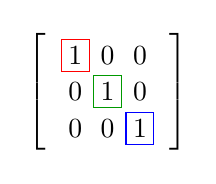
\begin{tikzpicture}[baseline=(m-2-2.base)]
            \matrix [matrix of math nodes,left delimiter={[},right delimiter={]}] (m)
            {
                1 & 0 & 0\\
                0 & 1 & 0\\
                0 & 0 & 1\\
            };
            \node[draw=red,inner sep=-1pt,fit=(m-1-1)(m-1-1)] {};
            \node[draw=green!60!black,inner sep=-1pt,fit=(m-2-2)(m-2-2)] {};
            \node[draw=blue,inner sep=-1pt,fit=(m-3-3)(m-3-3)] {};
        \end{tikzpicture},
        M_{C_2} =
        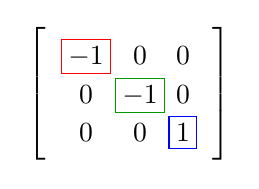
\begin{tikzpicture}[baseline=(m-2-2.base)]
            \matrix [matrix of math nodes,left delimiter={[},right delimiter={]}] (m)
            {
                -1 & 0 & 0\\
                0 & -1 & 0\\
                0 & 0 & 1\\
            };
            \node[draw=red,inner sep=-1pt,fit=(m-1-1)(m-1-1)] {};
            \node[draw=green!60!black,inner sep=-1pt,fit=(m-2-2)(m-2-2)] {};
            \node[draw=blue,inner sep=-1pt,fit=(m-3-3)(m-3-3)] {};
        \end{tikzpicture},
        M_{\sigma_{v1}} =
        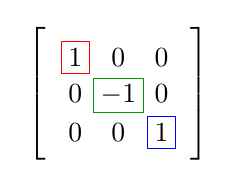
\begin{tikzpicture}[baseline=(m-2-2.base)]
            \matrix [matrix of math nodes,left delimiter={[},right delimiter={]}] (m)
            {
                1 & 0 & 0\\
                0 & -1 & 0\\
                0 & 0 & 1\\
            };
            \node[draw=red,inner sep=-1pt,fit=(m-1-1)(m-1-1)] {};
            \node[draw=green!60!black,inner sep=-1pt,fit=(m-2-2)(m-2-2)] {};
            \node[draw=blue,inner sep=-1pt,fit=(m-3-3)(m-3-3)] {};
        \end{tikzpicture},
        M_{\sigma_{v2}} =
        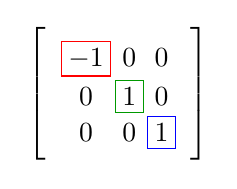
\begin{tikzpicture}[baseline=(m-2-2.base)]
            \matrix [matrix of math nodes,left delimiter={[},right delimiter={]}] (m)
            {
                -1 & 0 & 0\\
                0 & 1 & 0\\
                0 & 0 & 1\\
            };
            \node[draw=red,inner sep=-1pt,fit=(m-1-1)(m-1-1)] {};
            \node[draw=green!60!black,inner sep=-1pt,fit=(m-2-2)(m-2-2)] {};
            \node[draw=blue,inner sep=-1pt,fit=(m-3-3)(m-3-3)] {};
        \end{tikzpicture}
    \]
    
    We start building a character table by placing the traces of the first blocks in the first row ($x$), the traces of the second blocks in the second row ($y$), and the traces of the third blocks in the third row ($z$). The rows are color-coded to match their corresponding blocks for clarity. Of course, the trace of a $1\times 1$ block is a single element. Note that the $xz$ plane of the water molecule drawn above corresponds to $\sigma_{v1}$ in Table \ref{tab:c2vcayley}.

    With respect to the basis $\mathcal B_{xyz}$, each symmetry operation of $C_{2v}$ is represented by a diagonal matrix, so the three-dimensional representation decomposes into three one-dimensional subrepresentations. The rows labeled $(x), (y), (z)$ record the characters of these one-dimensional subrepresentations.

    \begin{table}[htbp]
        \centering
        \renewcommand{\arraystretch}{1.5}
        \begin{tabular}{c|cccc}
            $C_{2v}$ & $E$ & $C_2$ & $\sigma_{v1}~(xz)$ & $\sigma_{v2}~(yz)$\\
            \hline
            \color{red}$(x)$ & \color{red}$1$ & \color{red}$-1$ & \color{red}$1$ & \color{red}$-1$\\
            \color{green!60!black}$(y)$ & \color{green!60!black}$1$ & \color{green!60!black}$-1$ & \color{green!60!black}$-1$ & \color{green!60!black}$1$\\
            \color{blue}$(z)$ & \color{blue}$1$ & \color{blue}$1$ & \color{blue}$1$ & \color{blue}$1$
        \end{tabular}
    \end{table}

    Since $C_{2v}$ has four conjugacy classes, rule 3 tells us that there must be four irreps. Applying rules 6, 8, and 9, we find the characters of the fourth irrep. We now label the rows by the Mulliken symbols $A_1$, $A_2$, $B_1$, and $B_2$ by the aforementioned rules. By convention, we sort the rows by the Mulliken symbols.

    \begin{table}[htbp]
        \centering
        \renewcommand{\arraystretch}{1.5}
        \begin{tabular}{c|cccc}
            $C_{2v}$ & $E$ & $C_2$ & $\sigma_{v1}$ & $\sigma_{v2}$\\
            \hline
            $A_1$ & $1$ & $1$ & $1$ & $1$\\
            $A_2$ & $1$ & $1$ & $-1$ & $-1$\\
            $B_1$ & $1$ & $-1$ & $1$ & $-1$\\
            $B_2$ & $1$ & $-1$ & $-1$ & $1$\\
        \end{tabular}
    \end{table}
    
    We now have a complete character table for $C_{2v}$.
    
    To construct the character table for $C_{3v}$, observe that the representation matrices for $C_{3v}$ found in section \ref{sec:matricesc2vc3v}, with respect to the basis $\mathcal B_{xyz}$, are in block-diagonal form. Note that we need each matrix to have the same block sizes. Since the $C_{3v}$ matrices are not all diagonal, we need $2\times2$ and $1\times1$ blocks so that every nonzero element is within a block and that the blocks are as small as possible. Here we visually identify the blocks with color-coded boxes.
    \label{sec:c3vblocks}
    
    \[
        M_E =
        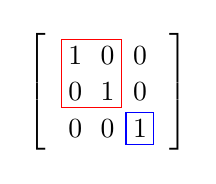
\begin{tikzpicture}[baseline=(m-2-2.base)]
            \matrix [matrix of math nodes,left delimiter={[},right delimiter={]}] (m)
            {
                1 & 0 & 0\\
                0 & 1 & 0\\
                0 & 0 & 1\\
            };
            \node[draw=red,inner sep=-1pt,fit=(m-1-1)(m-2-2)] {};
            \node[draw=blue,inner sep=-1pt,fit=(m-3-3)(m-3-3)] {};
        \end{tikzpicture},
        M_{C_3} =
        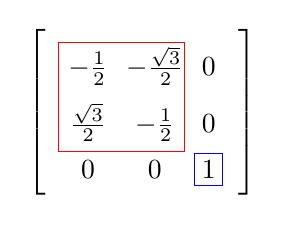
\begin{tikzpicture}[baseline=(m-2-2.base)]
            \matrix [matrix of math nodes,left delimiter={[},right delimiter={]}] (m)
            {
                -\frac12 & -\frac{\sqrt3}2 & 0\\
                \frac{\sqrt3}2 & -\frac12 & 0\\
                0 & 0 & 1\\
            };
            \node[draw=red,inner sep=0pt,fit=(m-1-1)(m-2-2)] {};
            \node[draw=blue,inner sep=-1pt,fit=(m-3-3)(m-3-3)] {};
        \end{tikzpicture},
        M_{C_3^2} =
        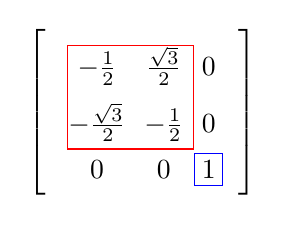
\begin{tikzpicture}[baseline=(m-2-2.base)]
            \matrix [matrix of math nodes,left delimiter={[},right delimiter={]}] (m)
            {
                -\frac12 & \frac{\sqrt3}2 & 0\\
                -\frac{\sqrt3}2 & -\frac12 & 0\\
                0 & 0 & 1\\
            };
            \node[draw=red,inner xsep=0pt,inner ysep=-1pt,fit=(m-1-1)(m-2-2)] {};
            \node[draw=blue,inner sep=-1pt,fit=(m-3-3)(m-3-3)] {};
        \end{tikzpicture},
    \]
    \[  
        M_{\sigma_{v1}} =
        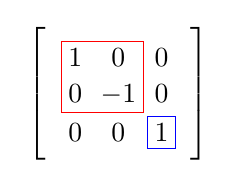
\begin{tikzpicture}[baseline=(m-2-2.base)]
            \matrix [matrix of math nodes,left delimiter={[},right delimiter={]}] (m)
            {
                1 & 0 & 0\\
                0 & -1 & 0\\
                0 & 0 & 1\\
            };
            \node[draw=red,inner sep=-1pt,fit=(m-1-1)(m-2-2)] {};
            \node[draw=blue,inner sep=-1pt,fit=(m-3-3)(m-3-3)] {};
        \end{tikzpicture},
        M_{\sigma_{v2}} =
        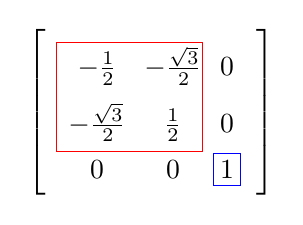
\begin{tikzpicture}[baseline=(m-2-2.base)]
            \matrix [matrix of math nodes,left delimiter={[},right delimiter={]}] (m)
            {
                -\frac12 & -\frac{\sqrt3}2 & 0\\
                -\frac{\sqrt3}2 & \frac12 & 0\\
                0 & 0 & 1\\
            };
            \node[draw=red,inner xsep=4pt,inner ysep=0pt,fit=(m-1-1)(m-2-2)] {};
            \node[draw=blue,inner sep=-1pt,fit=(m-3-3)(m-3-3)] {};
        \end{tikzpicture},
        M_{\sigma_{v3}} =
        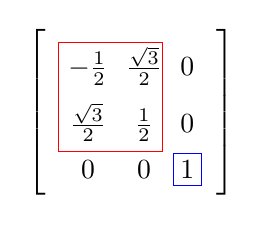
\begin{tikzpicture}[baseline=(m-2-2.base)]
            \matrix [matrix of math nodes,left delimiter={[},right delimiter={]}] (m)
            {
                -\frac12 & \frac{\sqrt3}2 & 0\\
                \frac{\sqrt3}2 & \frac12 & 0\\
                0 & 0 & 1\\
            };
            \node[draw=red,inner sep=0pt,fit=(m-1-1)(m-2-2)] {};
            \node[draw=blue,inner sep=-1pt,fit=(m-3-3)(m-3-3)] {};
        \end{tikzpicture}
    \]

    We start building a character table by placing the traces of the first blocks in the first row ($x, y$) and the traces of the second block in the second row ($z$). The $C_3$ and $C_3^2$ operations are in the same conjugacy class, and likewise the three $\sigma_v$ operations are in the same class, so they are grouped together in the character table. The rows are color-coded to match their corresponding blocks for clarity.

    With respect to the basis $\mathcal B_{xyz}$, each symmetry operation of $C_{3v}$ is represented by a block-diagonal matrix with $2\times2$ and $1\times1$ blocks, so the three-dimensional representation decomposes into a two-dimensional subrepresentation and a one-dimensional subrepresentation. The rows labeled $(x,y), (z)$ record the characters of these subrepresentations, respectively.

    \begin{table}[htbp]
        \centering
        \renewcommand{\arraystretch}{1.5}
        \begin{tabular}{c|ccc}
            $C_{3v}$ & $E$ & $2C_3$ & $3\sigma_{v}$\\
            \hline
            \color{red}$(x,y)$ & \color{red}$2$ & \color{red}$-1$ & \color{red}$0$\\
            \color{blue}$(z)$ & \color{blue}$1$ & \color{blue}$1$ & \color{blue}$1$
        \end{tabular}
    \end{table}
    
    Since $C_{3v}$ has three conjugacy classes, rule 3 tells us that there must be three irreps. Applying rules 6, 8, and 9, we find the characters of the third irrep. We now label the rows by the Mulliken symbols $A_1$, $A_2$, and $E$ by the aforementioned rules, sorting rows by the Mulliken symbols.
    
    \begin{table}[htbp]
        \centering
        \renewcommand{\arraystretch}{1.5}
        \begin{tabular}{c|ccc}
            $C_{3v}$ & $E$ & $2C_3$ & $3\sigma_{v}$\\
            \hline
            $A_1$ & $1$ & $1$ & $1$\\
            $A_2$ & $1$ & $1$ & $-1$\\
            $E$ & $2$ & $-1$ & $0$\\
        \end{tabular}
    \end{table}

    We now have a complete character table for $C_{3v}$.

    Notice that the character table has a row labeled $E$ for the two-dimensional irrep and a column labeled $E$ for the identity operation. This can be confusing, but it is the convention used for character tables in chemistry. This paper follows the conventional notation. In the discussion that follows, when we refer to $E$ without specification, we are referring to the identity operation.

    We could have also found the character table for $C_{3v}$ by using the basis $\beta$ as described in section \ref{sec:salcs}. Notice that the matrices $[M_i]_\gamma=P[M_i]_\beta P^\top$ that were found in that section have the same block-diagonal structure as the matrices with respect to the basis $\mathcal B_{xyz}$ (although with the order of the blocks reversed), and the resulting character table would be identical.

    \subsection{Decomposition of representations into irreducible representations}

    Now that we have constructed explicit matrix representations for the symmetry operations of the point groups $C_{2v}$ and $C_{3v}$, we decompose these representations as a direct sum of irreducible representations using the character tables we have constructed.

    Let $G$ be a point group. Let $\Gamma$ be a reducible representation of $G$. Let $\Gamma^{(i)}$ be an irreducible representation (irrep) of $G$. Let $\chi^{(i)}(C)$ represent the character of $\Gamma^{(i)}$ on the conjugacy class $C$. Let $n_C$ be the multiplicity of class $C$.

    We have \begin{equation}\Gamma \cong \bigoplus_i m_i \Gamma^{(i)},\label{eq:directsum}\end{equation}
    where \[m_i\Gamma^{(i)}=\underbrace{\Gamma^{(i)}\oplus\Gamma^{(i)}\oplus\cdots\oplus\Gamma^{(i)}}_{m_i \text{ times}},\] and where the multiplicity $m_i$ of $\Gamma^{(i)}$ is given by \begin{equation}m_i = \frac1{|G|} \sum_{C} n_C\chi^\Gamma(C)\overline{\chi^{(i)}(C)},\label{eq:irrepmultiplicity}\end{equation} where the sum is taken over all of the conjugacy classes. Note that \eqref{eq:irrepmultiplicity} is based on the same inner product formula as \eqref{eq:orthog} in section \ref{sec:propchar} (property \ref{property:orthogonality}) used to show orthogonality of the characters of irreducible representations.

    We will decompose the matrix representation for $C_{2v}$ found in section \ref{sec:matricesc2vc3v}. Let $\Gamma_{C_{2v}}$ denote this representation. The characters of $\Gamma_{C_{2v}}$ are the traces of the matrices, given by
    \[
        \chi^{\Gamma_{C_{2v}}}(E)=3,\quad
        \chi^{\Gamma_{C_{2v}}}(C_2)=-1,\quad
        \chi^{\Gamma_{C_{2v}}}(\sigma_{v1})=1,\quad
        \chi^{\Gamma_{C_{2v}}}(\sigma_{v2})=1.
    \]

    Recall that the order of the point group $C_{2v}$ is $4$. Also, recall that the conjugacy classes of $C_{2v}$ are the singleton sets $\{E\}, \{C_2\}, \{\sigma_{v1}\}, \{\sigma_{v2}\}$, so we have \[n_E=n_{C_2}=n_{\sigma_{v1}}=n_{\sigma_{v2}}=1.\] Using the values in the character table of $C_{2v}$, we compute the multiplicities of the irreps using \eqref{eq:irrepmultiplicity}:
    \begin{align*}m_{A_1}&=\frac14 \sum_{C} n_C\chi^{\Gamma_{C_{2v}}}(C)\overline{\chi^{A_1}(C)}\\&=\frac14\left(n_E\chi^{\Gamma_{C_{2v}}}(E)\overline{\chi^{A_1}(E)}+n_{C_2}\chi^{\Gamma_{C_{2v}}}(C_2)\overline{\chi^{A_1}(C_2)}+n_{\sigma_{v1}}\chi^{\Gamma_{C_{2v}}}(\sigma_{v1})\overline{\chi^{A_1}(\sigma_{v1})}+n_{\sigma_{v2}}\chi^{\Gamma_{C_{2v}}}(\sigma_{v2})\overline{\chi^{A_1}(\sigma_{v2})}\right)\\&=\frac14\left(1\cdot3\cdot1+1\cdot(-1)\cdot1+1\cdot1\cdot1+1\cdot1\cdot1\right)=1.\end{align*}
    Similarly, we compute $m_{A_2} = 0$, $m_{B_1} = 1$, and $m_{B_2} = 1$.

    Thus, by \eqref{eq:directsum}, we have
    \[
        \Gamma_{C_{2v}} \cong A_1 \oplus B_1 \oplus B_2.
    \]

    We will also decompose the matrix representation for $C_{3v}$, with respect to the basis $\mathcal B_{xyz}$, found in section \ref{sec:matricesc2vc3v}. Let $\Gamma_{C_{3v}}$ denote this representation. The characters of $\Gamma_{C_{3v}}$ are the traces of the matrices, given by
    \[
        \chi^{\Gamma_{C_{3v}}}(E)=3,\quad
        \chi^{\Gamma_{C_{3v}}}(C_3)=0,\quad
        \chi^{\Gamma_{C_{3v}}}(C_3^2)=0,\quad
        \chi^{\Gamma_{C_{3v}}}(\sigma_{v1})=1,\quad
        \chi^{\Gamma_{C_{3v}}}(\sigma_{v2})=1,\quad
        \chi^{\Gamma_{C_{3v}}}(\sigma_{v3})=1.
    \]

    Recall that the order of the point group $C_{3v}$ is $6$. Also, recall that the conjugacy classes in $C_{3v}$ are the sets $\{E\}, \{C_3,C_3^2\},$ and $\{\sigma_{v1},\sigma_{v2},\sigma_{v3}\}$, and we label these as $E$, $C_3$, and $\sigma_v$, respectively, so we have \[n_E=1,\quad n_{C_3}=2,\quad n_{\sigma_v}=3.\] Using the values in the character table of $C_{3v}$, we compute the multiplicities of the irreps using \eqref{eq:irrepmultiplicity}:
    \begin{align*}m_{A_1}&=\frac16 \sum_{C} n_C\chi^{\Gamma_{C_{3v}}}(C)\overline{\chi^{A_1}(C)}\\&=\frac16\left(n_{E}\chi^{\Gamma_{C_{3v}}}(E)\overline{\chi^{A_1}(E)}+n_{C_3}\chi^{\Gamma_{C_{3v}}}(C_3)\overline{\chi^{A_1}(C_3)}+n_{\sigma_v}\chi^{\Gamma_{C_{3v}}}(\sigma_{v})\overline{\chi^{A_1}(\sigma_{v})}\right)\\&=\frac16\left(1\cdot3\cdot1+2\cdot0\cdot1+3\cdot1\cdot1\right)=1.\end{align*}
    Similarly, we compute $m_{A_2} = 0$ and $m_{E} = 1$.

    Thus, by \eqref{eq:directsum}, we have
    \[
        \Gamma_{C_{3v}} \cong A_1 \oplus E.
    \]

    We have now decomposed the matrix representations for the point groups $C_{2v}$ and $C_{3v}$ into direct sums of irreducible representations using their character tables. The multiplicities obtained from \eqref{eq:irrepmultiplicity} agree with the block structure observed when the representations are expressed in a symmetry-adapted basis. In this basis, the representation matrices are block-diagonal, with each block corresponding to an irreducible component. This shows that the character-theoretic decomposition captures the same underlying structure as the explicit change of basis, providing a systematic and basis-independent method for identifying irreducible components.

    \section{Eigenvalues of representations of \texorpdfstring{$C_{2v}$ and $C_{3v}$}{C2v and C3v}}

    Now that we have constructed the character tables for $C_{2v}$ and $C_{3v}$, we notice that all of the characters we have found so far are in the integer set $\{-1,0,1,2\}$. At this point, we may ask if there are point groups for which other integers appear as characters, or indeed if there are point groups with non-integer characters. To begin investigating which types of numbers may appear as characters, we will do some linear algebra on the symmetry operation matrices for $C_{2v}$ and $C_{3v}$. In particular, we will find their characteristic polynomials, eigenvalues, and minimal polynomials. Surprisingly, this analysis will open the door to cyclotomic field structures and Galois actions, which will reveal some of the algebraic number theory behind the characters.

    First, we recall some definitions from linear algebra. Let $A$ be an $n\times n$ matrix. Let $I_n$ denote the $n\times n$ identity matrix and $O_n$ the $n\times n$ zero matrix. The characteristic polynomial $p_A(x)$ of $A$ is defined by \[p_A(x)=\det(xI_n-A),\] where $I_n$ is the $n\times n$ identity matrix. The eigenvalues of $A$ are the roots of $p_A(x)$, and the algebraic multiplicity of each eigenvalue is the multiplicity of the root of $p_A(x)$. Each eigenvalue $\lambda_i$ of $A$ satisfies the equation $Av_i=\lambda_iv_i$ for some vector $v_i\neq 0$. The vector $v_i$ is called the eigenvector corresponding to $\lambda_i$. The minimal polynomial $m_{A}(x)$ of an $n\times n$ matrix $A$ is the monic polynomial of least positive degree such that $m_{A}(A)=O_n$. \cite{friedberg2018linear} By the Cayley-Hamilton theorem, every matrix satisfies its own characteristic polynomial, i.e., $p_A(A)=O_n$. The minimal polynomial divides the characteristic polynomial and has the same roots, but without repeated factors beyond those that are necessary to annihilate the matrix.
    
    To better understand the structure of the point group representation matrices for $C_{2v}$ and $C_{3v}$, we now find their characteristic polynomials, eigenvalues, and minimal polynomials.

    Recall that the matrices for the symmetry operations of $C_{2v}$ are \[M_E=\begin{bmatrix}1&0&0\\0&1&0\\0&0&1\end{bmatrix}, M_{C_2}=\begin{bmatrix}-1&0&0\\0&-1&0\\0&0&1\end{bmatrix}, M_{\sigma_{v1}}=\begin{bmatrix}1&0&0\\0&-1&0\\0&0&1\end{bmatrix}, \text{ and } M_{\sigma_{v2}}=\begin{bmatrix}-1&0&0\\0&1&0\\0&0&1\end{bmatrix}.\]

    \pagebreak

    For each of these matrices $M_i$, we calculate the characteristic polynomials $p_{M_i}(x)$, eigenvalues with multiplicities, and minimal polynomials $m_{M_i}(x)$. For example, for the matrix $M_{C_2}$, we find $p_{M_{C_2}}(x)=\det(xI_3-M_{C_2})$, where $I_3$ is the $3\times 3$ identity matrix, which gives
    \[p_{M_{C_2}}(x)=\det\begin{bmatrix}x+1&0&0\\0&x+1&0\\0&0&x-1\end{bmatrix}=(x+1)^2(x-1).\]
    
    The eigenvalues of $M_{C_2}$ are the roots of $p_{M_{C_2}}(x)$, which are $x=1$, with algebraic multiplicity 1, and $x=-1$, with algebraic multiplicity 2. The minimal polynomial of $M_{C_2}$ is $m_{M_{C_2}}(x)=(x-1)(x+1)$, since $m_{M_{C_2}}(M_{C_2})=O_3$, $m_{M_{C_2}}(x)\mid p_{M_{C_2}}(x)$, and neither $x-1$ nor $x+1$ annihilates $M_{C_2}$.
    
    Note that the minimal polynomial $m_{M_{C_2}}(x)$ can be expressed as a product of cyclotomic polynomials $\Phi_1(x)\Phi_2(x)$, where $\Phi_1(x)=x-1$ and $\Phi_2(x)=x+1$. We will prove that the minimal polynomial is a product of cyclotomic polynomials in the following section.

    By performing similar calculations, we can find the characteristic polynomials, eigenvalues with algebraic multiplicities, and the minimal polynomials for all of the matrices in the point group $C_{2v}$. These results are summarized in Table \ref{tab:c2vpoly}.

    \begin{table}[p]
        \centering
        \renewcommand{\arraystretch}{3.5}
        \begin{tabular}{cccc}
            Matrix $M_i$ & Char. polynomial $p_{M_i}(x)$ & Eigenvalues (alg. mult.) & Minimal polynomial $m_{M_i}(x)$\\
            \hline
            $M_E$ & $(x-1)^3$ & $1$ (3) & $x-1=\Phi_1(x)$\\[5mm]
            $M_{C_2}$ & $(x-1)(x+1)^2$ & $1$ (1), $-1$ (2) & $(x-1)(x+1)=\Phi_1(x)\Phi_2(x)$\\[5mm]
            $M_{\sigma_{v1}}, M_{\sigma_{v2}}$ & $(x-1)^2(x+1)$ & $1$ (2), $-1$ (1) & $(x-1)(x+1)=\Phi_1(x)\Phi_2(x)$
        \end{tabular}
        \caption{Characteristic polynomials, eigenvalues (and their algebraic multiplicities), and minimal polynomials for the matrices in the point group $C_{2v}$.}
        \label{tab:c2vpoly}
    \end{table}

    The minimal polynomials in $C_{2v}$ are $m_{M_E}(x)=\Phi_1(x)$ and $m_{M_{C_2}}(x)=m_{M_{\sigma_{v1}}}(x)=m_{M_{\sigma_{v2}}}(x)=\Phi_1(x)\Phi_2(x)$.

    Recall that the matrices for the symmetry operations of $C_{3v}$ (with the basis $\mathcal B_{xyz}$) are \[M_E=\begin{bmatrix}1&0&0\\0&1&0\\0&0&1\end{bmatrix}, M_{C_3}=\begin{bmatrix}-\frac12&-\frac{\sqrt{3}}2&0\\\frac{\sqrt{3}}2&-\frac12&0\\0&0&1\end{bmatrix}, M_{C_3^2}=\begin{bmatrix}-\frac12&\frac{\sqrt{3}}2&0\\-\frac{\sqrt{3}}2&-\frac12&0\\0&0&1\end{bmatrix},\]
    \[M_{\sigma_{v1}}=\begin{bmatrix}1&0&0\\0&-1&0\\0&0&1\end{bmatrix}, M_{\sigma_{v2}}=\begin{bmatrix}-\frac12&-\frac{\sqrt{3}}2&0\\-\frac{\sqrt3}2&\frac12&0\\0&0&1\end{bmatrix}, \text{ and } M_{\sigma_{v3}}=\begin{bmatrix}-\frac12&\frac{\sqrt{3}}2&0\\\frac{\sqrt3}2&\frac12&0\\0&0&1\end{bmatrix}.\]

    For each of these matrices $M_i$, we calculate the characteristic polynomials $p_{M_i}(x)$, eigenvalues with algebraic multiplicities, and minimal polynomials $m_{M_i}(x)$, as we did with $C_{2v}$ above. The results are summarized in Table \ref{tab:c3vpoly}.

    \begin{table}[htbp]
        \centering
        \renewcommand{\arraystretch}{3.5}
        \begin{tabular}{cccc}
            Matrix $M_i$ & Char. polynomial $p_{M_i}(x)$ & Eigenvalues (alg. mult.) & Minimal polynomial $m_{M_i}(x)$\\
            \hline
            $M_E$ & $(x-1)^3$ & $1$ (3) & $x-1=\Phi_1(x)$\\[5mm]
            $M_{C_3}, M_{C_3^2}$ & $(x-1)(x^2+x+1)$ & \parbox{3cm}{\centering $1$ (1),\\~\\ $-\dfrac12+\dfrac{\sqrt{3}}{2}i$ (1),\\~\\ $-\dfrac12-\dfrac{\sqrt{3}}{2}i$ (1)} & $(x-1)(x^2+x+1)=\Phi_1(x)\Phi_3(x)$\\[5mm]
            $M_{\sigma_{v1}}, M_{\sigma_{v2}}, M_{\sigma_{v3}}$ & $(x-1)^2(x+1)$ & $1$ (2), $-1$ (1) & $(x-1)(x+1)=\Phi_1(x)\Phi_2(x)$
        \end{tabular}
        \caption{Characteristic polynomials, eigenvalues (and their algebraic multiplicities), and minimal polynomials for the matrices in the point group $C_{3v}$.}
        \label{tab:c3vpoly}
    \end{table}

    The minimal polynomials in $C_{3v}$ are $m_{M_E}(x)=\Phi_1(x)$, $m_{M_{C_3}}(x)=m_{M_{C_3^2}}(x)=\Phi_1(x)\Phi_3(x)$, and $m_{M_{\sigma_{v1}}}(x)=m_{M_{\sigma_{v2}}}(x)=m_{M_{\sigma_{v3}}}(x)=\Phi_1(x)\Phi_2(x)$.

    \pagebreak

    \section{Cyclotomic field structures of point group representations}

    To generalize the observations made in the last section, we state the following standard results, which we tailor to the present context. Our goal is to understand the number-theoretic basis of the character tables. We begin by establishing a relationship between finite symmetry group elements and cyclotomic fields.
    \begin{proposition}
        Let $G$ be a finite point group, and let $g\in G$ be an element of order $n$. Let $\rho:G\to GL(V)$ be a representation of $G$. Then every eigenvalue of $\rho(g)$ is an $n$th root of unity and hence lies in a cyclotomic field $\mathbb{Q}(\zeta_n)$.
        \label{prop:eigcyc}
    \end{proposition}
    \begin{proof}
        We have $g^n=e$, where $e$ denotes the identity element of $G$. Applying the representation $\rho$, we have $\rho(g)^n=\rho(e)=I$, where $I$ is an identity matrix. Let $\lambda$ be an eigenvalue of $\rho(g)$ with associated eigenvector $v\neq0$. Then $\rho(g)v=\lambda v$. Applying $\rho(g)$ to $v$ twice, we have \[(\rho(g))^2v=\rho(g)(\rho(g)v)=\rho(g)(\lambda v)=\lambda(\lambda v)=\lambda^2v.\] By an induction argument, we can see that $(\rho(g))^nv=\lambda^nv$. We also have $(\rho(g))^n=I$, so $(\rho(g))^nv=Iv=v$. Hence $\lambda^nv=v$, so $(\lambda^n-1)v=0$, and since $v\neq0$, we have $\lambda^n=1$. Since $\lambda$ was arbitrary, every eigenvalue of $\rho(g)$ is an $n$th root of unity. Hence it lies in a cyclotomic field $\mathbb{Q}(\zeta_n)$.
    \end{proof}

    As a direct consequence of Proposition \ref{prop:eigcyc}, we see why the minimal polynomials lie in cyclotomic fields.

    \begin{proposition}
        Let $G$ be a finite point group, and let $g\in G$ be an element of order $n$. Let $\rho:G\to GL(V)$ be a representation of $G$. Then the minimal polynomial of $\rho(g)$ splits in a cyclotomic field $\mathbb{Q}(\zeta_n)$.
        \label{prop:minpolycyc}
    \end{proposition}
    \begin{proof}
        By Proposition \ref{prop:eigcyc}, the eigenvalues of $\rho(g)$ lie in a cyclotomic field $\mathbb{Q}(\zeta_n)$. Hence, the characteristic polynomial of $\rho(g)$ splits in $\mathbb{Q}(\zeta_n)$. Since for any matrix, the minimal polynomial is a factor of the characteristic polynomial, the minimal polynomial splits in $\mathbb{Q}(\zeta_n)$ as well.
    \end{proof}

    We can strengthen the result of Proposition \ref{prop:minpolycyc} by showing that the minimal polynomial is a product of cyclotomic polynomials.

    \enlargethispage{\baselineskip}

    \begin{proposition}
        Let $G$ be a finite point group, and let $g\in G$ be an element of order $n$. Let $\rho:G\to GL(V)$ be a representation of $G$. Then the minimal polynomial of $\rho(g)$ is a product of cyclotomic polynomials.
        \label{prop:minpolycycpoly}
    \end{proposition}
    \begin{proof}
        We have $g^n=e$, where $e$ denotes the identity element of $G$. Then $(\rho(g))^n=I$, so $(\rho(g))^n-I=O$, where $I$ is an identity matrix and $O$ is a zero matrix. Hence $\rho(g)$ satisfies the polynomial equation $x^n-1=0$. Let $m_{\rho(g)}(x)$ be the minimal polynomial of $\rho(g)$. Then $m_{\rho(g)}(x)\mid (x^n-1)$. We have that \[x^n-1=\prod_{d\mid n}\Phi_d(x),\] where $\Phi_d(x)$ is the $d$th cyclotomic polynomial. Since $m_{\rho(g)}(x)\mid(x^n-1)$, \[m_{\rho(g)}(x)~\bigg\lvert~\prod_{d\mid n}\Phi_d(x).\] We have that $\mathbb{Q}[x]$ is a unique factorization domain, since $\mathbb{Q}$ is a field. \cite{dummit} Furthermore, each $\Phi_d(x)$ is irreducible in $\mathbb{Q}[x]$. \cite{sanna} Thus \[x^n-1=\prod_{d\mid n}\Phi_d(x),\] as the factorization of $x^n-1$ into cyclotomic polynomials in $\mathbb{Q}[x]$, is in particular the factorization of $x^n-1$ into irreducible polynomials in $\mathbb{Q}[x]$. So any divisor of $x^n-1$, in particular $m_{\rho(g)}(x)$, is a product of cyclotomic polynomials.
    \end{proof}

    We will now see that the entries of character tables lie in cyclotomic fields. To do this, we will show that characters of representations, in particular irreducible representations, are sums of $n$th roots of unity.

    \begin{proposition}
        Let $G$ be a finite point group, and let $g\in G$ be an element of order $n$. Let $\rho : G\to GL(V)$ be an irreducible representation of $G$ with character $\chi$. Then $\chi(g)$ is a sum of $n$th roots of unity. In particular, $\chi(g)\in\mathbb{Q}(\zeta_n)$.
        \label{prop:charcyc}
    \end{proposition}
    \begin{proof}
        Since $\rho$ is an irreducible representation of $G$, it is in particular a representation of $G$. By Proposition \ref{prop:eigcyc}, every eigenvalue of $\rho(g)$ is an $n$th root of unity. Since $\chi(g)=\tr(\rho(g))$, and the trace of a matrix is the sum of its eigenvalues, it follows that $\chi(g)$ is the sum of $n$th roots of unity. Thus, $\chi(g)\in\mathbb{Q}(\zeta_n)$.
    \end{proof}

    \subsection{Cyclotomic field structure of \texorpdfstring{$C_{3v}$}{C3v}}

    We will now analyze the eigenvalues and minimal polynomials for the rotation matrices $M_{C_3}$ and $M_{C_3^2}$ of $C_{3v}$ shown in Table \ref{tab:c3vpoly}. Let $\omega$ be a primitive third root of unity; that is,
    \[\omega=-\dfrac{1}{2}+\frac{\sqrt{3}}{2}i=e^{2\pi i/3}.\]
    Then the complex conjugate of $\omega$ is \[\overline\omega=-\dfrac{1}{2}-\frac{\sqrt{3}}{2}i=e^{4\pi i/3}=\omega^2.\]
    Note that $\omega\overline\omega = \omega^3 = e^{2\pi i}=1\in\mathbb{R}$ and $\omega+\overline\omega = -1\in\mathbb{R}$.

    With this in hand, we see that the eigenvalues of $M_{C_3}$ and $M_{C_3^2}$ are $1,\omega$, and $\omega^2$, so the eigenvalues lie in the cyclotomic field $\mathbb{Q}(\omega)$.

    The cyclotomic polynomial $\Phi_3(x)=x^2+x+1$ is the minimal polynomial of the third root of unity $\omega=e^{2\pi i/3}$. To see this, we use the fact that $\omega^3=1$, so that $\omega^3-1=0$. Factoring, we have $(\omega-1)(\omega^2+\omega+1)=0$. Since $\omega\neq1$, we must have $\omega^2+\omega+1=0$. Hence $\Phi_3(\omega)=0$.

    As was previously noted, the minimal polynomial of $M_{C_3}$, denoted $m_{M_{C_3}}$, is the product of cyclotomic polynomials $\Phi_1(x)\Phi_3(x)$. We see that $m_{M_{C_3}}$ splits in the field $\mathbb{Q}(\omega)$, for we can write \[m_{M_{C_3}}=(x-1)(x^2+x+1)=(x-1)(x-\omega)(x-\omega^2).\] (The same discussion applies for $M_{C_3^2}$, since $m_{M_{C_3}}=m_{M_{C_3^2}}$.)

    \subsection{Cyclotomic field structure of \texorpdfstring{$C_{2v}$}{C2v}}

    Using the same framework, we can also analyze the eigenvalues and minimal polynomials for the rotation matrix $M_{C_2}$ of $C_{2v}$ shown in Table \ref{tab:c2vpoly}. Let $\psi$ be a primitive second root of unity; that is,
    \[\psi=-1=e^{2\pi i/2}.\]
    In particular, note that $\psi\in\mathbb{R}$ and $\psi^2=1\in\mathbb{R}$.

    The eigenvalues of $M_{C_2}$ are $1$ and $\psi$, so the eigenvalues lie in the cyclotomic field $\mathbb{Q}(\psi)$. However, $\psi=-1$, so $\mathbb{Q}(\psi)\subseteq\mathbb{R}$. Hence the eigenvalues are real.
    
    The cyclotomic polynomial $\Phi_2(x)=x+1$ is the minimal polynomial of the second root of unity $\psi=-1$. The minimal polynomial of $M_{C_2}$, denoted $m_{M_{C_2}}$, is the product of cyclotomic polynomials $\Phi_1(x)\Phi_2(x)$. We see that $m_{M_{C_2}}$ splits in $\mathbb{Q}(\psi)$, so it also splits in $\mathbb{R}$.

    \subsection{Summary of cyclotomic field structures of \texorpdfstring{$C_{2v}$ and $C_{3v}$}{C2v and C3v}}

    Note that for both $C_{2v}$ and $C_{3v}$, the mirror plane symmetries $M_{\sigma_{vi}}$ have eigenvalues $\pm1$, which lie in the cyclotomic field $\mathbb{Q}(\zeta_2)$, and the minimal polynomials $m_{M_{\sigma_{vi}}}$ split in $\mathbb{Q}(\zeta_2)$.

    By Proposition \ref{prop:eigcyc}, the eigenvalues of the matrices for the $C_n$ rotational symmetry operations lie in $\mathbb{Q}(\zeta_n)$. By Proposition \ref{prop:minpolycyc}, their minimal polynomials split over $\mathbb{Q}(\zeta_n)$. The minimal polynomial splits over $\mathbb{R}$ if and only if all eigenvalues real, in which case $\mathbb{Q}(\zeta_n)\subseteq\mathbb{R}$. The only $n$ values for which this happens are $n=1$ and $n=2$, since for any $n>2$, $e^{2\pi i/n}\in\mathbb{C}\setminus\mathbb{R}$. Hence, the only nontrivial rotational symmetry operation for which the eigenvalues are real ($\lambda=\pm1$) is $C_2$.

    In particular, the rotation operator in $C_{2v}$ has eigenvalues in $\mathbb{R}$, and its minimal polynomial splits in $\mathbb{R}$. However, the rotation operators in $C_{3v}$ have eigenvalues in $\mathbb{Q}(\omega)\not\subseteq\mathbb{R}$, and their minimal polynomials split in $\mathbb{Q}(\omega)\not\subseteq\mathbb{R}$.

    \section{Galois actions on point group representations}

    By Proposition \ref{prop:charcyc}, we have that the characters of finite group elements lie in a cyclotomic field. That is an interesting result, but it does not tell the whole story. To this point, let us take another look at the character tables of $C_{2v}$ and $C_{3v}$.

    \begin{table}[htbp]
        \centering
        \renewcommand{\arraystretch}{1.5}
        \begin{tabular}{c p{1cm} c}
            \begin{tabular}{c|cccc}
                $C_{2v}$ & $E$ & $C_2$ & $\sigma_{v1}$ & $\sigma_{v2}$\\
                \hline
                $A_1$ & $1$ & $1$ & $1$ & $1$\\
                $A_2$ & $1$ & $1$ & $-1$ & $-1$\\
                $B_1$ & $1$ & $-1$ & $1$ & $-1$\\
                $B_2$ & $1$ & $-1$ & $-1$ & $1$\\
            \end{tabular}&&
            \begin{tabular}{c|ccc}
                $C_{3v}$ & $E$ & $2C_3$ & $3\sigma_{v}$\\
                \hline
                $A_1$ & $1$ & $1$ & $1$\\
                $A_2$ & $1$ & $1$ & $-1$\\
                $E$ & $2$ & $-1$ & $0$\\
            \end{tabular}\\
        \end{tabular}
    \end{table}

    \pagebreak

    We see that all of the characters in these two point groups are integers. For $C_{2v}$, this is expected, since characters are sums of eigenvalues, and all of the eigenvalues of the matrices in $C_{2v}$ are integers, as seen in Table \ref{tab:c2vpoly}. However, for $C_{3v}$, this is surprising, since the eigenvalues of the $C_3$ and $C_3^2$ matrices in $C_{3v}$ lie in $\mathbb{Q}(\zeta_3)$ and are not all integers, as seen in Table \ref{tab:c3vpoly}. We will investigate why these characters are integers. To do so, we will consider Galois actions on the eigenvalues of the point group matrices.

    To understand the action of Galois automorphisms on primitive $n$th roots of unity and on eigenvalues, we state the following standard results, which we tailor to the present context.

    \begin{proposition}
        Let $U$ be the set of primitive $n$th roots of unity, let $\psi\in U$, and let $G=\Gal(\mathbb{Q}(\psi)/\mathbb{Q})$ be the Galois group of field automorphisms of $\mathbb{Q}(\psi)$ that fix $\mathbb{Q}$. For every $1\le k < n$ such that $\gcd(k,n)=1$, there exists an element $\sigma_k\in G$ such that $\sigma_k(\psi)=\psi^k$.
        \label{prop:allprimitiverootsofunityarehit}
    \end{proposition}

    \begin{proof}
        Let $\sigma\in G$ be arbitrary. Since $\mathbb{Q}(\psi)$ is generated by $\psi$ over $\mathbb{Q}$, every element of $\mathbb{Q}(\psi)$ can be written as a polynomial in $\psi$ with rational coefficients. That is, for arbitrary $x\in\mathbb{Q}(\psi)$, we have \[x = a_0+a_1\psi+a_2\psi^2+\cdots,\] where $a_0,a_1,\ldots\in\mathbb{Q}$. Because $\sigma$ fixes $\mathbb{Q}$ and preserves addition and multiplication, applying $\sigma$ to $x$ gives
        \begin{align*}
            \sigma(x) &= \sigma(a_0 + a_1\psi+a_2\psi^2+\cdots)\\
            &=\sigma(a_0) + \sigma(a_1)\sigma(\psi) + \sigma(a_2)(\sigma(\psi^2))+\cdots\\
            &=a_0+a_1\sigma(\psi)+a_2(\sigma(\psi))^2+\cdots.
        \end{align*}
        Hence, once we know $\sigma(\psi)$, we know $\sigma(\psi^2), \sigma(\psi^3),\cdots$. Thus the action of $\sigma$ on $\mathbb{Q}(\psi)$ is completely determined by $\sigma(\psi)$.
        
        Since $\psi\in U$, it satisfies $\psi^n-1=0$. By acting on both sides of this equation by $\sigma$, we have $\sigma(\psi^n-1)=\sigma(0)=0$. Since $\sigma$ preserves addition and multiplication, we have $(\sigma(\psi))^n-1=0$. Hence $\sigma(\psi)$ is an $n$th root of unity. We claim that $\sigma(\psi)$ is a \emph{primitive} $n$th root of unity, i.e., $\sigma(\psi)\in U$. Assume to the contrary that $\sigma(\psi)\notin U$, so $(\sigma(\psi))^d=1$ for some $d<n$. Then applying the automorphism $\sigma^{-1}$ to both sides, we have $\sigma^{-1}(\sigma(\psi))^d=\sigma^{-1}(1)$. Since $\sigma$ preserves multiplication, we have $\psi^d=1$. However, $\psi\in U$, so $d\geq n$. This is a contradiction, so $\sigma(\psi)\in U$.
    
        Since $\psi\in U$, we have that \[G=\Gal(\mathbb{Q}(\psi)/\mathbb{Q})\cong(\mathbb{Z}/n\mathbb{Z})^{\times},\] where $(\mathbb{Z}/n\mathbb{Z})^\times$ consists of all classes mod $n$ of integers coprime to $n$. \cite{dummit,gannon} Hence, \[|G|=|(\mathbb{Z}/n\mathbb{Z})^\times|=\varphi(n),\] where $\varphi$ is the Euler totient function. Now, we also have that there are exactly $\varphi(n)$ primitive $n$th roots of unity, i.e., $|U|=\varphi(n)$. So $|G|=|U|$. It remains to show that there is a bijection from $G$ to $U$. We have that an injection between finite sets of equal cardinality is a bijection. Since $|G|=|U|$, it suffices to show there is an injection from $G$ into $U$.
        
        Let $\sigma_1,\sigma_2\in G$. Suppose $\sigma_1(\psi) = \sigma_2(\psi)$. For arbitrary $x \in \mathbb{Q}(\psi)$, we have $x = a_0+a_1\psi+a_2\psi^2+\cdots$, where $a_0,a_1,\ldots\in\mathbb{Q}$. Applying $\sigma_1$ to $x$ gives \[\sigma_1(x)=\sigma_1(a_0 + a_1\psi+a_2\psi^2+\cdots).\] Likewise, applying $\sigma_2$ to $x$ gives \[\sigma_2(x)=\sigma_2(a_0 + a_1\psi+a_2\psi^2+\cdots).\] Because $\sigma_1$ and $\sigma_2$ fix $\mathbb{Q}$ and preserve addition and multiplication, we have \[\sigma_1(x) = a_0 + a_1\sigma_1(\psi) + a_2(\sigma_1(\psi))^2+\cdots,\] and \[\sigma_2(x) = a_0 + a_1\sigma_2(\psi) + a_2(\sigma_2(\psi))^2+\cdots.\] Since $\sigma_1(\psi)=\sigma_2(\psi)$, we have $\sigma_1(x)=\sigma_2(x)$. However, $x$ was arbitrary, so $\sigma_1=\sigma_2$. Thus, the mapping from $G$ to $U$ is injective, and hence bijective.
        
        Therefore, for every $1\le k < n$ such that $\gcd(k,n)=1$, there exists an element $\sigma_k\in G$ such that $\sigma_k(\psi)=\psi^k$.
    \end{proof}

    \begin{proposition}
        Let $A$ be a matrix whose characteristic polynomial $p_A(x)$ lies in $\mathbb{Q}[x]$. If $\lambda_1,\lambda_2,\ldots,\lambda_n$ are the eigenvalues of $A$ in a splitting field $K$ of $p_A(x)$, then every Galois automorphism $\sigma\in\Gal(K/\mathbb{Q})$ permutes the eigenvalues. \label{prop:galoispermuteeigs}
    \end{proposition}

    \begin{proof}
        Since $A$ has $n$ eigenvalues (counting multiplicities), $p_A(x)$ has degree $n$. We have that $p_A(x)=a_0+a_1x+a_2x^2+\cdots+a_nx^n$, where $a_0, a_1, \ldots a_n\in\mathbb{Q}$. Since the eigenvalues are roots of $p_A(x)$, we have \[a_0+a_1\lambda_i+a_2\lambda_i^2+\cdots+a_n\lambda_i^n=0,\] for all $i = 1,\ldots, n$. Applying $\sigma$ to both sides, we have \[\sigma(a_0+a_1\lambda_i+a_2\lambda_i^2+\cdots+a_n\lambda_i^n)=\sigma(0).\] Since $\sigma$ fixes $\mathbb{Q}$ and preserves addition and multiplication, we have \[a_0+a_1\sigma(\lambda_i)+a_2(\sigma(\lambda_i))^2+\cdots+a_n(\sigma(\lambda_i))^n=0.\] Hence $\sigma(\lambda_i)$ is also a root of $p_A(x)$, so it is an eigenvalue of $A$. Hence $\sigma(\lambda_i)=\lambda_j$ for some $j\in\{1,\ldots,n\}$. Since automorphisms are bijective by definition, $\sigma$ permutes the eigenvalues. \cite{conrad}
    \end{proof}

    \subsection{Galois actions on \texorpdfstring{$C_{3v}$}{C3v}}

    We now apply Proposition \ref{prop:galoispermuteeigs} to the two-dimensional irreducible representation $E$ of $C_{3v}$. From the block-diagonal form of the $C_{3v}$ matrices in section \ref{sec:c3vblocks} on page \pageref{sec:c3vblocks}, the irrep $E$ corresponds to the upper-left $2\times 2$ block of each representation matrix. In particular, the $2\times2$ blocks of $M_{C_3}$ and $M_{C_3^2}$ have eigenvalues $\omega$ and $\omega^2$, where $\omega=e^{2\pi i/3}$ is a primitive third root of unity. Also, these blocks have the characteristic polynomial $x^2+x+1$, which has rational coefficients. The eigenvalues $\omega,\omega^2$ lie in the splitting field $\mathbb{Q}(\omega)$ of $x^2+x+1$.

    Let $g$ be the matrix representing a $C_3$ rotational operation in the point group $C_{3v}$, and let $g'$ denote the $2\times2$ block of $g$ corresponding to the irrep $E$. The character $\chi^E(g)$ is the trace of the matrix $g'$, and the trace of a matrix is the sum of its eigenvalues. If $g'$ has the eigenvalue multiset $\Lambda$, then \[\chi^E(g)=\tr(g')=\sum_{\lambda\in\Lambda}\lambda.\] Since the characteristic polynomial of $g'$ lies in $\mathbb{Q}[x]$ and splits in $\mathbb{Q}(\omega)$, Proposition \ref{prop:galoispermuteeigs} implies that the Galois automorphism $\sigma\in\Gal(\mathbb{Q}(\omega)/\mathbb{Q})$ permutes the eigenvalues of $g'$. Therefore $\sigma$ permutes the multiset $\Lambda$, and hence fixes its sum. Thus,
    \[
        \sigma(\chi^E(g))=\sigma\left(\sum_{\lambda\in\Lambda}\lambda\right)=\sum_{\lambda\in\Lambda}\sigma(\lambda)=\sum_{\lambda\in\Lambda}\lambda=\chi^E(g).
    \]
    Thus, the character is fixed by $\sigma$, so $\chi^E(g)\in\mathbb{Q}$.
    
    The invariance of the sum of the eigenvalue multiset $\Lambda$ under the Galois automorphism $\sigma\in\Gal(\mathbb{Q}(\omega)/\mathbb{Q})$ forces the characters to lie in $\mathbb{Q}$. Since characters are sums of roots of unity, they are algebraic integers. The only rational algebraic integers are the ordinary integers. Thus $\chi^E(g)\in\mathbb{Z}$. \cite{roche}

    In particular, for the $C_3$ conjugacy class in $C_{3v}$, we obtain
    \[\chi^E(C_3)=\omega+\omega^2=-1.\]

    There is a geometric interpretation of this result. In the two-dimensional irreducible representations, the $C_3$ operation acts as a rotation by $120^\circ$ in the plane. The eigenvalues of a rotation by $\theta$ are $e^{i\theta}$ and $e^{-i\theta}$, so the trace is \[\chi^E(C_3)=e^{i\theta}+e^{-i\theta}=2\cos\theta.\] When $\theta=120^\circ$, \[\chi^E(C_3)=2\cos120^\circ=-1,\] which agrees with the cyclotomic computation $\omega+\omega^2=-1$.

    \pagebreak

    \subsection{Galois actions on fivefold symmetry point groups}

    By the previous discussion, one may wonder if characters are always integers for every chemistry-relevant point group. The answer is no, as seen in the character tables for the point groups $C_{5v}$, $D_5$, $D_{5d}$, and $D_{5h}$ in Tables \ref{tab:c5v}-\ref{tab:d5h}. These character tables are presented without full derivation, due to their relative complexity. These point groups all have fivefold rotational symmetry operations in common. We will see the relevance of these point groups in chemistry after we discuss their mathematical structure.

    \begin{table}[p]
        \centering
        \renewcommand{\arraystretch}{1.5}
        \begin{minipage}{0.45\textwidth}
            \centering
            \begin{tabular}{c|cccc}
                $C_{5v}$ & $E$ & $2C_5$ & $2C_5^2$ & $5\sigma_v$\\
                \hline
                $A_1$ & $1$ & $1$ & $1$ & $1$\\
                $A_2$ & $1$ & $1$ & $1$ & $-1$\\
                $E_1$ & $2$ & $-\frac12+\frac{\sqrt{5}}{2}$ & $-\frac12-\frac{\sqrt{5}}{2}$ & $0$\\
                $E_2$ & $2$ & $-\frac12-\frac{\sqrt{5}}{2}$ & $-\frac12+\frac{\sqrt{5}}{2}$ & $0$\\
            \end{tabular}
            \caption{The character table of the point group $C_{5v}$. \cite{miessler2014}}
            \label{tab:c5v}
        \end{minipage}
        \hfill
        \begin{minipage}{0.45\textwidth}
            \centering
            \begin{tabular}{c|cccc}
                $D_{5}$ & $E$ & $2C_5$ & $2C_5^2$ & $5C_2$\\
                \hline
                $A_1$ & $1$ & $1$ & $1$ & $1$\\
                $A_2$ & $1$ & $1$ & $1$ & $-1$\\
                $E_1$ & $2$ & $-\frac12+\frac{\sqrt{5}}{2}$ & $-\frac12-\frac{\sqrt{5}}{2}$ & $0$\\
                $E_2$ & $2$ & $-\frac12-\frac{\sqrt{5}}{2}$ & $-\frac12+\frac{\sqrt{5}}{2}$ & $0$\\
            \end{tabular}
            \caption{The character table of the point group $D_5$. \cite{miessler2014}}
            \label{tab:d5}
        \end{minipage}
    \end{table}

    \begin{table}[htbp]
        \centering
        \renewcommand{\arraystretch}{1.5}
        \begin{tabular}{c|cccccccc}
            $D_{5d}$ & $E$ & $2C_5$ & $2C_5^2$ & $5C_2$ & $i$ & $2S_{10}^3$ & $2S_{10}$ & $5\sigma_d$\\
            \hline
            $A_{1g}$ & $1$ & $1$ & $1$ & $1$ & $1$ & $1$ & $1$ & $1$\\
            $A_{2g}$ & $1$ & $1$ & $1$ & $-1$ & $1$ & $1$ & $1$ & $-1$\\
            $E_{1g}$ & $2$ & $-\frac12+\frac{\sqrt{5}}{2}$ & $-\frac12-\frac{\sqrt{5}}{2}$ & $0$ & $2$ & $-\frac12+\frac{\sqrt{5}}{2}$ & $-\frac12-\frac{\sqrt{5}}{2}$ & $0$\\
            $E_{2g}$ & $2$ & $-\frac12-\frac{\sqrt{5}}{2}$ & $-\frac12+\frac{\sqrt{5}}{2}$ & $0$ & $2$ & $-\frac12-\frac{\sqrt{5}}{2}$ & $-\frac12+\frac{\sqrt{5}}{2}$ & $0$\\
            $A_{1u}$ & $1$ & $1$ & $1$ & $1$ & $-1$ & $-1$ & $-1$ & $-1$\\
            $A_{2u}$ & $1$ & $1$ & $1$ & $-1$ & $-1$ & $-1$ & $-1$ & $1$\\
            $E_{1u}$ & $2$ & $-\frac12+\frac{\sqrt{5}}{2}$ & $-\frac12-\frac{\sqrt{5}}{2}$ & $0$ & $-2$ & $\frac12-\frac{\sqrt{5}}{2}$ & $\frac12+\frac{\sqrt{5}}{2}$ & $0$\\
            $E_{2u}$ & $2$ & $-\frac12-\frac{\sqrt{5}}{2}$ & $-\frac12+\frac{\sqrt{5}}{2}$ & $0$ & $-2$ & $\frac12+\frac{\sqrt{5}}{2}$ & $\frac12-\frac{\sqrt{5}}{2}$ & $0$\\
        \end{tabular}
        \caption{The character table of the point group $D_{5d}$. \cite{miessler2014} Refer to section \ref{sec:mulliken} on page \pageref{sec:mulliken} for a discussion of the $g$ (\emph{gerade}) and $u$ (\emph{ungerade}) notation used here.}
        \label{tab:d5d}
    \end{table}

    \begin{table}[htbp]
        \centering
        \renewcommand{\arraystretch}{1.5}
        \begin{tabular}{c|cccccccc}
            $D_{5h}$ & $E$ & $2C_5$ & $2C_5^2$ & $5C_2$ & $\sigma_h$ & $2S_5$ & $2S_5^3$ & $5\sigma_v$\\
            \hline
            $A_1'$ & $1$ & $1$ & $1$ & $1$ & $1$ & $1$ & $1$ & $1$\\
            $A_2'$ & $1$ & $1$ & $1$ & $-1$ & $1$ & $1$ & $1$ & $-1$\\
            $E_1'$ & $2$ & $-\frac12+\frac{\sqrt{5}}{2}$ & $-\frac12-\frac{\sqrt{5}}{2}$ & $0$ & $2$ & $-\frac12+\frac{\sqrt{5}}{2}$ & $-\frac12-\frac{\sqrt{5}}{2}$ & $0$\\
            $E_2'$ & $2$ & $-\frac12-\frac{\sqrt{5}}{2}$ & $-\frac12+\frac{\sqrt{5}}{2}$ & $0$ & $2$ & $-\frac12-\frac{\sqrt{5}}{2}$ & $-\frac12+\frac{\sqrt{5}}{2}$ & $0$\\
            $A_1''$ & $1$ & $1$ & $1$ & $1$ & $-1$ & $-1$ & $-1$ & $-1$\\
            $A_2''$ & $1$ & $1$ & $1$ & $-1$ & $-1$ & $-1$ & $-1$ & $1$\\
            $E_1''$ & $2$ & $-\frac12+\frac{\sqrt{5}}{2}$ & $-\frac12-\frac{\sqrt{5}}{2}$ & $0$ & $-2$ & $\frac12-\frac{\sqrt{5}}{2}$ & $\frac12+\frac{\sqrt{5}}{2}$ & $0$\\
            $E_2''$ & $2$ & $-\frac12-\frac{\sqrt{5}}{2}$ & $-\frac12+\frac{\sqrt{5}}{2}$ & $0$ & $-2$ & $\frac12+\frac{\sqrt{5}}{2}$ & $\frac12-\frac{\sqrt{5}}{2}$ & $0$\\
        \end{tabular}
        \caption{The character table of the point group $D_{5h}$. \cite{miessler2014} Refer to section \ref{sec:mulliken} on page \pageref{sec:mulliken} for a discussion of the $'$ (\emph{single prime}) and $''$ (\emph{double prime}) notation used here.}
        \label{tab:d5h}
    \end{table}

    In the character tables for $C_{5v}$, $D_5$, $D_{5d}$, and $D_{5h}$, some of the characters for the $C_5$ rotational symmetry (as well as the $C_5^2$, $S_{10}$, $S_{10}^3$, $S_5$, and $S_5^3$ symmetries) are irrational numbers lying in the field $\mathbb{Q}(\sqrt{5})$. In particular, these characters are of the form \[\pm\dfrac12\pm\dfrac{\sqrt{5}}{2},\] although not all sign choices appear in each column. Interestingly, these characters can be written in the form $\pm\varphi$ or $\pm\dfrac{1}{\varphi}$, where $\varphi=\dfrac12+\dfrac{\sqrt5}{2}$ is the golden ratio. Using the framework established in the previous sections, we will investigate why the characters of the $C_5$ rotational symmetry operation are not all integers.

    Let $\xi=e^{2\pi i/5}$ be a primitive fifth root of unity. By Proposition \ref{prop:eigcyc}, any eigenvalue of the $C_5$ operation must be in the set $\{1, \xi, \xi^2, \xi^3, \xi^4\}$ within the cyclotomic field $\mathbb{Q}(\zeta_5)=\mathbb{Q}(\xi)$.

    In the point groups $C_{5v}$, $D_5$, $D_{5d}$, and $D_{5h}$, the irrational characters occur in the two-dimensional irreps $E_1$ and $E_2$ (or $E_{1g}$, etc.). For a $C_5$-type operation in these point groups, the character of a two-dimensional irrep is the trace of the corresponding $2\times 2$ block, namely the sum of its two eigenvalues.

    For any real matrix $A$, if $\lambda$ is an eigenvalue, then the conjugate $\overline\lambda$ is also an eigenvalue, for if we have $Av=\lambda v$ for some eigenvector $v\neq 0$, we can take the conjugate of both sides to get $A\overline v=\overline\lambda \overline v$.
    
    A $C_5$ rotational symmetry operation can be expressed as a real matrix, such as \[\begin{bmatrix}\cos 72^\circ&-\sin72^\circ&0\\\sin72^\circ&\cos72^\circ&0\\0&0&1\end{bmatrix}.\] The two-dimensional irrep corresponds to a $2\times 2$ real-valued block of this matrix. Therefore, if $\xi^k$ is an eigenvalue of this block, then the conjugate $\xi^{-k}$ is also an eigenvalue. We have two possible eigenvalue conjugate pairs; either $\xi$ and $\xi^{-1}=\xi^4$, or $\xi^2$ and $\xi^{-2}=\xi^3$.
    
    By Proposition \ref{prop:allprimitiverootsofunityarehit}, the Galois automorphisms of the cyclotomic field $\mathbb{Q}(\xi)$ are given by $\sigma_k(\xi)=\xi^k$, for every $k$ coprime to $5$. Since $\varphi(5)=4$, there are four automorphisms in the Galois group $G=\Gal(\mathbb{Q}(\xi)/\mathbb{Q})$, which are given by
    \[\sigma_k(\xi)=\xi^k, \text{where } k=1,2,3,4.\]
    
    \pagebreak
    
    We see that the automorphism $\sigma_4\in G$ acts as complex conjugation, since $\sigma_4(\xi)=\xi^4$ and $\sigma_4(\xi^2)=\xi^8=\xi^3$. Denote $\sigma_4$ as $\tau$, the complex conjugation automorphism. Hence, under $\tau$, we have $\xi\mapsto\xi^4$ and $\xi^2\mapsto\xi^3$. We have, since automorphisms preserve addition and multiplication, \[\tau(\xi+\xi^4)=\tau(\xi)+(\tau(\xi))^4=\xi^4+(\xi^4)^4=\xi^4+\xi^{16}=\xi^4+\xi,\] and \[\tau(\xi^2+\xi^3)=(\tau(\xi))^2+(\tau(\xi))^3=(\xi^4)^2+(\xi^4)^3=\xi^8+\xi^{12}=\xi^3+\xi^2.\] Since $\xi+\xi^4$ and $\xi^2+\xi^3$ are invariant under $\tau$ (complex conjugation), we have that $\xi+\xi^4\in\mathbb{R}$ and $\xi^2+\xi^3\in\mathbb{R}$. Furthermore, we compute \[\xi+\xi^4=-\frac12+\frac{\sqrt5}{2}\] and \[\xi^2+\xi^3=-\frac12-\frac{\sqrt5}{2},\] which lie in $\mathbb{Q}(\sqrt{5})$ but not in $\mathbb{Q}$. In fact, as seen in the $C_5$ column of Tables \ref{tab:c5v}-\ref{tab:d5}, these two sums occur in distinct two-dimensional irreducible representations.

    We can also verify that $\xi+\xi^4$ and $\xi^2+\xi^3$ are not rational by considering their orbits under $G$. The orbit of $\xi+\xi^4$ is \[\{\sigma(\xi+\xi^4)\mid \sigma\in G\}.\] Calculations similar to the preceding ones show that the orbit is $\{\xi+\xi^4,\xi^2+\xi^3\}$. We have that rational numbers are fixed by every element of $G$. Since $\xi+\xi^4$ is not fixed by every element of $G$, it is not rational. Similarly, $\xi^2+\xi^3$ is not rational.

    In the case of $C_{3v}$, the Galois automorphism $\sigma$ permutes the conjugate eigenvalues $\omega$ and $\omega^2$, and their sum is the integer $\omega + \omega^2=-1$.

    In contrast, for $C_{5v}$, $D_5$, $D_{5d}$, and $D_{5h}$, the Galois automorphism $\tau$ permutes the conjugate pairs $\xi, \xi^4$ and $\xi^2, \xi^3$. In the characters, the sums of the conjugate eigenvalues do not reduce to integers. Instead, the sums lie in $\mathbb{Q}(\sqrt{5})$ but not in $\mathbb{Q}$. The appearance of irrational values in the character tables of certain point groups therefore reflects the underlying cyclotomic field structure.

    The preceding analysis shows that the structure of molecular point group representations is governed by a combination of representation theory, cyclotomic fields, and Galois actions. We now return to the molecular setting to examine how this structure is realized in specific classes of point groups, where these abstract ideas are manifested concretely in the symmetry of actual molecules. In particular, we will focus on molecules that belong to the point groups $C_{5v}$, $D_5$, $D_{5d}$, and $D_{5h}$, with a discussion of certain molecules that can possess more than one symmetry group as they undergo dynamic rearrangement. We will also look at some molecules that belong to abelian point groups, such as $C_5$ and $C_3$.

    \pagebreak   

    \section{Molecular structures with special symmetries}

    \subsection{Molecules with fivefold symmetry}

    Molecules that belong to a point group with fivefold symmetry are not common, but they do exist. One interesting example is corannulene (\ch{C20H10}), seen in Figure \ref{fig:corannulene}. In its ground state, it belongs to the point group $C_{5v}$. Note that corannulene is a bowl-shaped molecule with carbon atoms arranged into five hexagons and one pentagon, and a bowl depth measured to be $0.875$~\AA~($8.75\times10^{-11}$ m). It consists of five interconnected benzene rings in a pentagonal arrangement. It is the smallest fragment of buckminsterfullerene (\ch{C60}) that has a curvature of the carbon framework (see section \ref{sec:bucky}). \cite{mattarella}

    \begin{figure}[htbp]
        \centering
        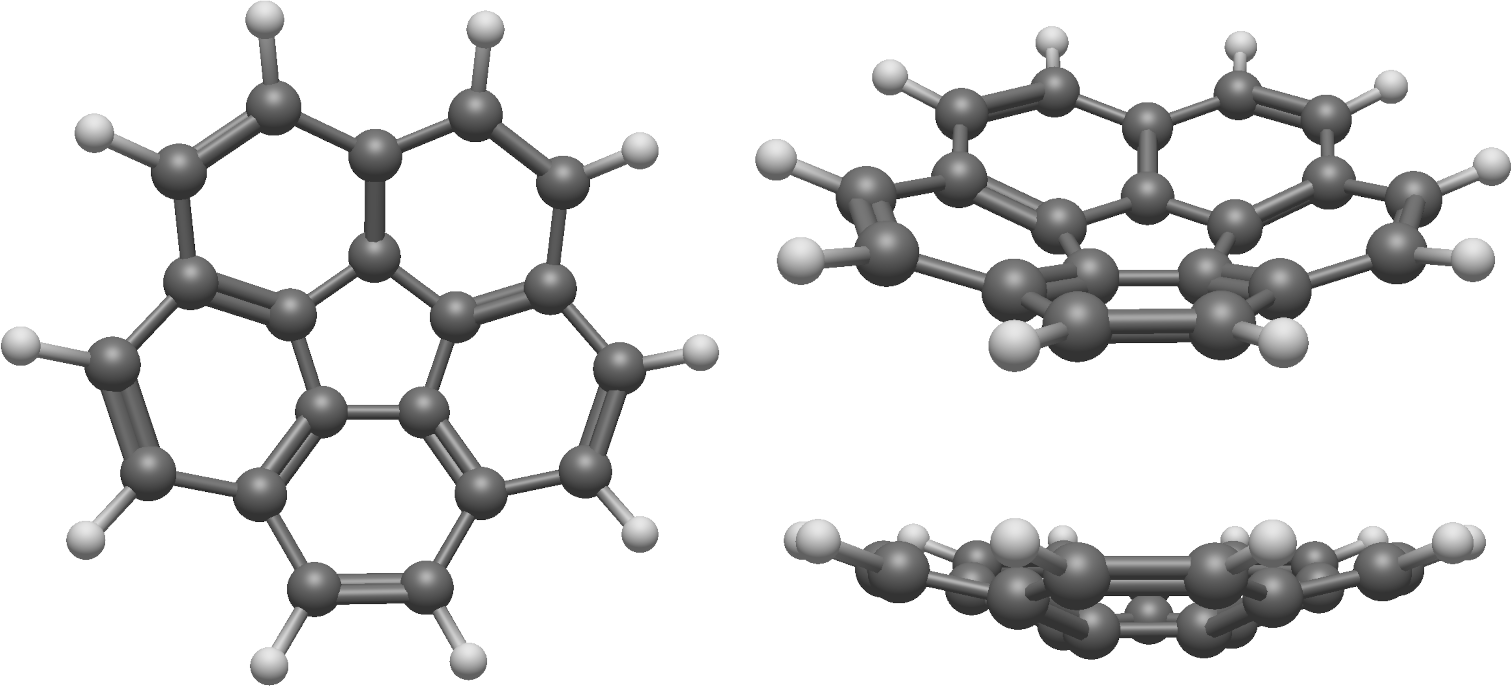
\includegraphics[width=\linewidth]{figures/corannulene.png}
        \caption{Structure of corannulene (\ch{C20H10}), a molecule with $C_{5v}$ symmetry in its ground state, shown from three different perspectives. Note that the carbon atoms are not coplanar in the ground state.}
        \label{fig:corannulene}
    \end{figure}

    Corannulene undergoes a bowl-to-bowl inversion process, where it passes through a high energy planar transition state, as seen in Figure \ref{fig:corannulenebowltobowl}. \cite{mattarella} In a sense, it can be thought of as a tiny umbrella that flips back and forth in the wind. The bowl-to-bowl inversion energy barrier has been measured to be $44.9 \text{ kJ mol}^{-1}$ ($10.7 \text{ kcal mol}^{-1}$). \cite{biedermann} Its transition state has $D_{5h}$ symmetry, which occurs precisely when it is exactly between the two bowl configurations. This is an interesting example of a phenomenon where molecular motion may momentarily change the point group to which a molecule belongs.

    \begin{figure}[p]
        \centering
        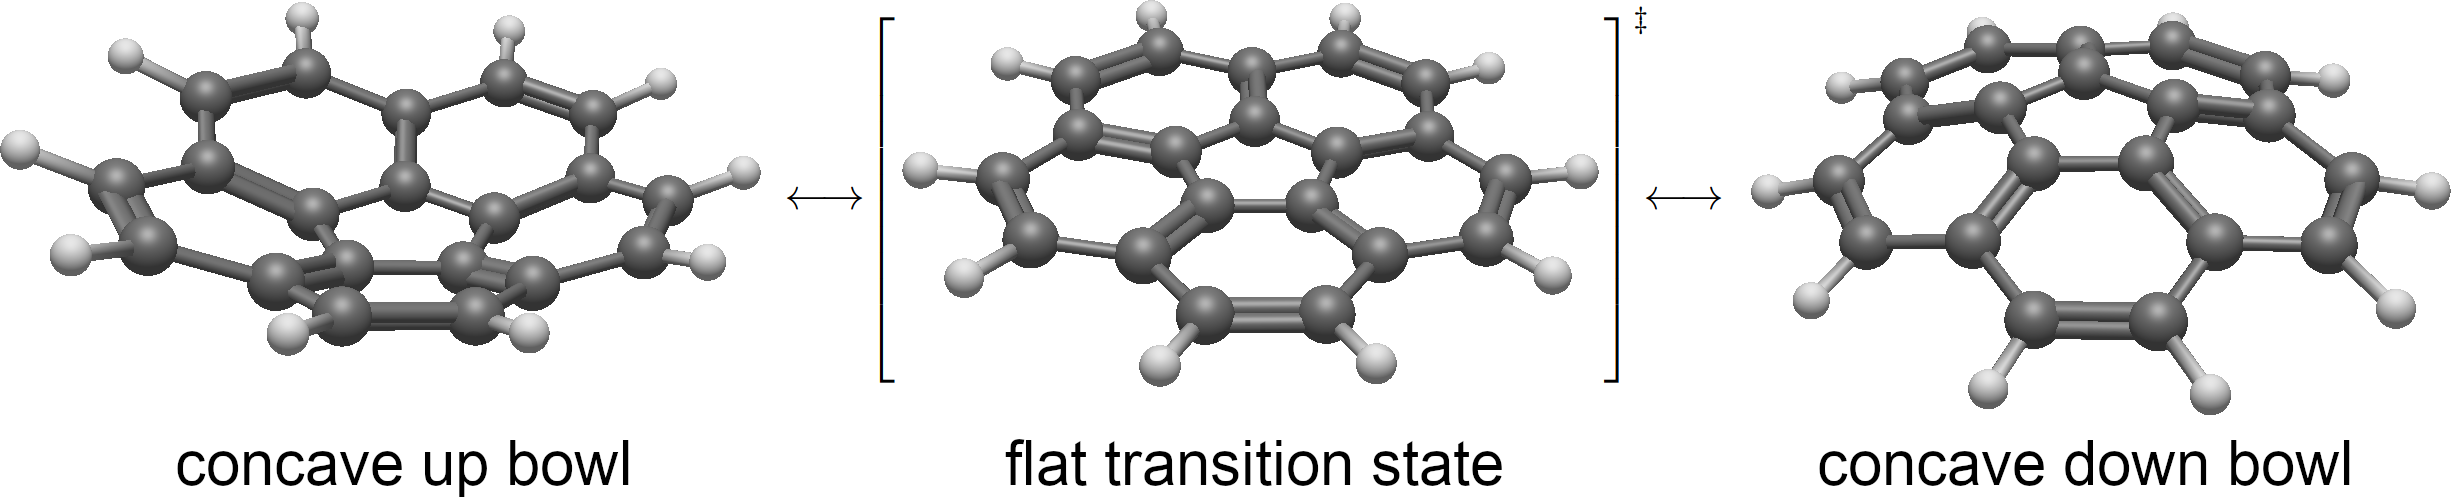
\includegraphics[width=\linewidth]{figures/corannulenebowltobowl.png}
        \caption{Bowl-to-bowl inversion of corannulene, showing the two ground-state bowl configurations with $C_{5v}$ symmetry and the flat transition state (denoted $\ddagger$) with $D_{5h}$ symmetry. \cite{sripaturad}}
        \label{fig:corannulenebowltobowl}
    \end{figure}

    \enlargethispage{\baselineskip}

    Adding or removing an electron from corannulene to form an ion also changes the point group to which it belongs. The neutral state of corannulene has a doubly degenerate HOMO (highest occupied molecular orbital) and LUMO (lowest unoccupied molecular orbital). Adding an electron to form a negative ion (anion) causes a partial filling of a doubly degenerate LUMO, and removing an electron to form a positive ion (cation) causes a partial filling of a doubly degenerate HOMO. Both of these situations result in a Jahn-Teller effect, where a molecule will undergo a geometric distortion to eliminate degeneracy, thereby reducing symmetry. See Figure \ref{fig:jahnteller}. For that reason, both cationic and anionic forms of corannulene belong to the point group $C_s$, which lacks rotational symmetry and only contains a single $\sigma_h$ mirror plane, in contrast to neutral corannulene. The character table for the point group $C_s$ is shown in Table \ref{tab:cs}. \cite{tampieri}

    \pagebreak

    \begin{figure}[p]
        \centering
        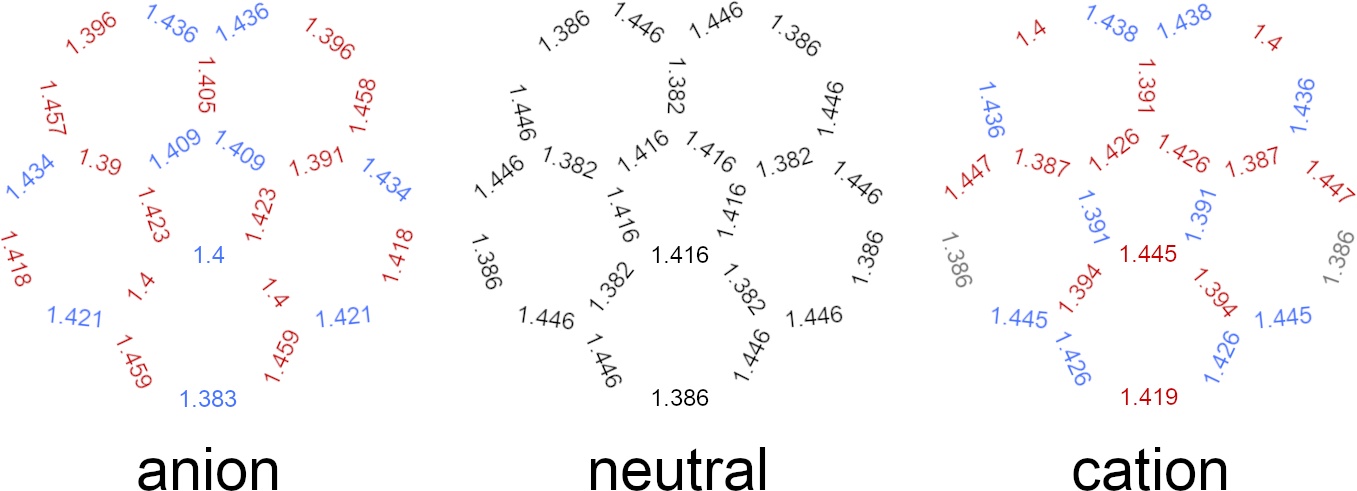
\includegraphics[width=\linewidth]{figures/jahnteller.png}
        \caption{Bond lengths of corannulene, in angstroms (\AA), in the anion form (left), neutral form (center), and cation form (right), illustrating the Jahn-Teller effect. (1 \AA ~= $10^{-10}$ m.) Calculated by Tampieri et al. using Density Functional Theory. Note that the distorted bond lengths in the anion and cation forms reduce the symmetry to the point group $C_s$, as compared to $C_{5v}$ for the neutral form. Colors indicate a change in bond length as compared to the neutral form (red: longer, blue: shorter, gray: no change at three decimal places). \cite{tampieri}}
        \label{fig:jahnteller}
    \end{figure}

    \begin{table}[p]
        \centering
        \renewcommand{\arraystretch}{1.5}
        \begin{tabular}{c|cc}
            $C_{s}$ & $E$ & $\sigma_h$\\
            \hline
            $A'$ & $1$ & $1$\\
            $A''$ & $1$ & $-1$
        \end{tabular}
        \caption{The character table of the point group $C_s$. \cite{miessler2014} Refer to section \ref{sec:mulliken} on page \pageref{sec:mulliken} for a discussion of the $'$ (\emph{single prime}) and $''$ (\emph{double prime}) notation used here.}
        \label{tab:cs}
    \end{table}

    \pagebreak
    \clearpage

    Another example of a molecule with fivefold symmetry is ferrocene (\ch{Fe(C5H5)2}), seen in its staggered and eclipsed conformations in Figure \ref{fig:ferrocene}. Ferrocene consists of two five-carbon rings that ``sandwich'' an iron atom. In the staggered conformation, the rings are rotated $36^\circ$ relative to each other, placing the carbon atoms of one ring between those of the other ring, and the molecule belongs to the point group $D_{5d}$. In the eclipsed conformation, the two rings are aligned in the same way, such that the carbon atoms of one ring are aligned with the carbon atoms of the other ring, and the molecule belongs to the point group $D_{5h}$. \cite{mohammadi} Along the rotational pathway between the staggered and eclipsed conformations, one may also consider an intermediate twisted configuration that belongs to the point group $D_5$, which has no mirror planes. The rotational energy barrier between the two conformations of ferrocene is only $4.2 \text{ kJ mol}^{-1}$ ($1.0 \text{ kcal mol}^{-1}$), meaning that the rotation of ferrocene occurs much more freely than the bowl-to-bowl inversion of corannulene. \cite{lunghi} This is another example where molecular motion can change the point group of a molecule.

    \begin{figure}[htbp]
        \centering
        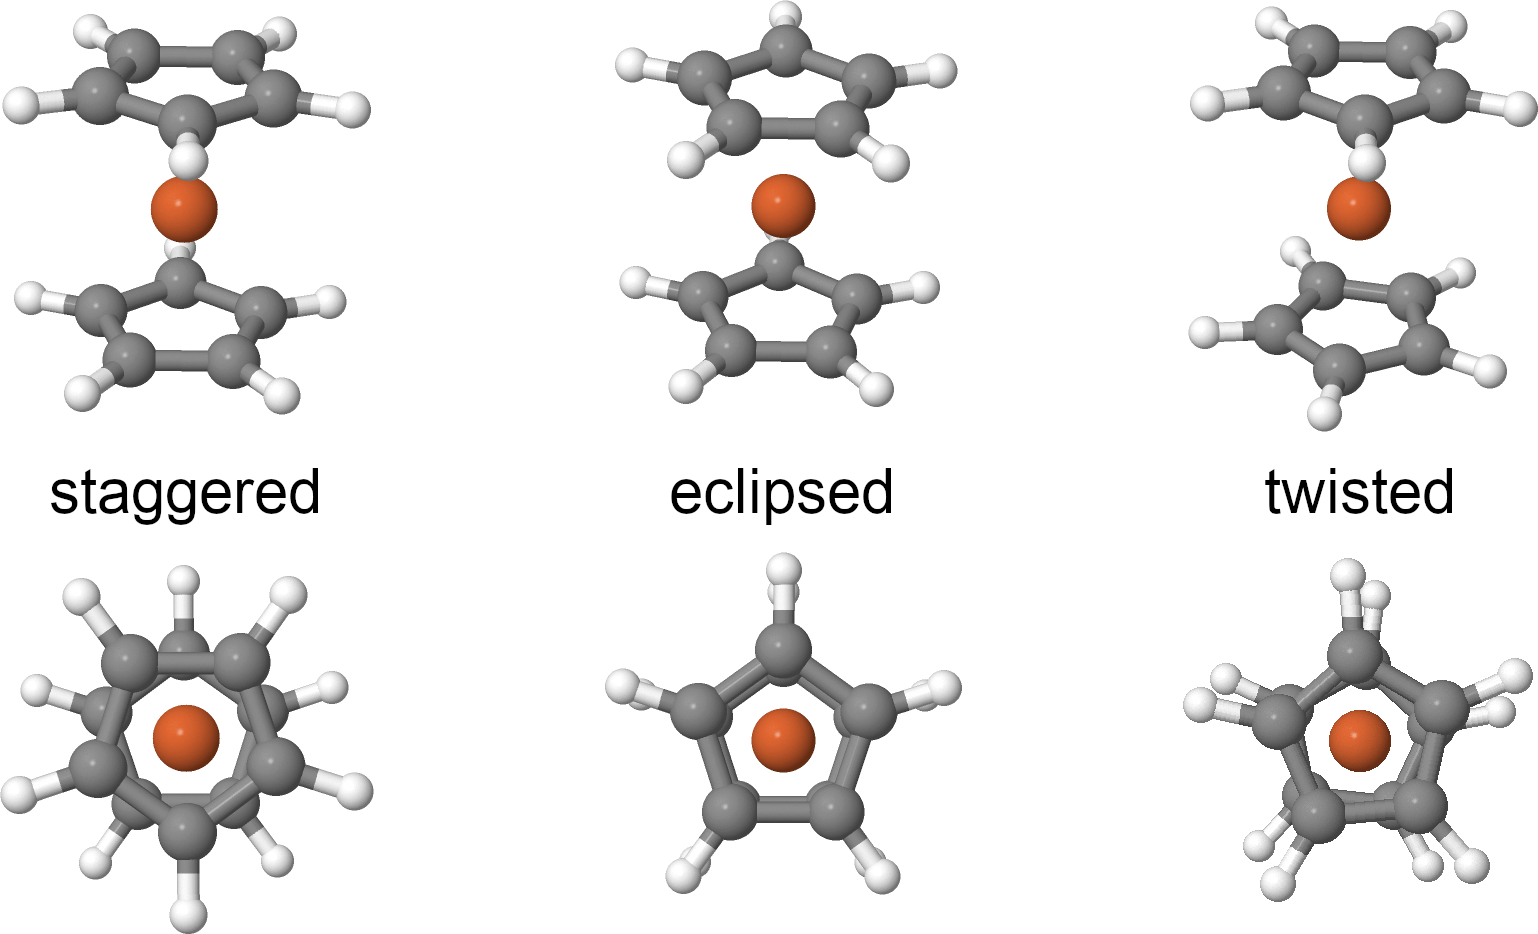
\includegraphics[width=\linewidth]{figures/ferrocene.png}
        \caption{Structure of ferrocene (\ch{Fe(C5H5)2}), a molecule with $D_{5d}$ symmetry in the staggered conformation (left), $D_{5h}$ symmetry in the eclipsed conformation (center), and $D_5$ symmetry in the twisted conformation (right). Each conformer is shown from two perspectives.}
        \label{fig:ferrocene}
    \end{figure}

    \subsection{Molecules belonging to abelian point groups}

    We cannot say that \emph{every} point group with fivefold symmetry has character values in $\mathbb{Q}(\sqrt{5})$. The point group $C_5$ is a counterexample. Here, $C_5$ is not referring to a fivefold rotational symmetry operation, but an entire point group, which contains no mirror planes, and no $C_2$ axes perpendicular to the principal $C_5$ axis. The point group $C_5$ is abelian, and it is a cyclic group of order $5$. Hence, all of its irreducible representations are one-dimensional, so the characters are fifth roots of unity rather than traces of two-dimensional real matrix blocks. That is, the characters lie in $\mathbb{Q}(\zeta_5)$, not $\mathbb{Q}(\sqrt{5})$. The character table for $C_5$ is shown in Table \ref{tab:c5}. Thus, the appearance of characters in $\mathbb{Q}(\sqrt{5})$ is a feature of point groups with suitable two-dimensional irreducible representations, such as $C_{5v}$, $D_5$, $D_{5d}$, and $D_{5h}$, but not of every point group that involves fivefold rotational symmetry. Molecules belonging to the point group $C_5$ are rare. One fascinating molecule belonging to the point group $C_5$ is 1,3,5,7,9-penta(ferrocenyl)corannulene (\ch{C20H5(C5H5FeC5H4)5}). This molecule consists of a corannulene structure to which five ferrocenyl functional groups are bonded. This molecule provides a concrete realization of the point group $C_5$, illustrating a case where the characters lie in the cyclotomic field $\mathbb{Q}(\zeta_5)$ rather than $\mathbb{Q}(\sqrt{5})$. A 3D rendering of this molecule is shown in Figure \ref{fig:fercor}. \cite{miessler2014,topolinski}

    \begin{figure}[htbp]
        \centering
        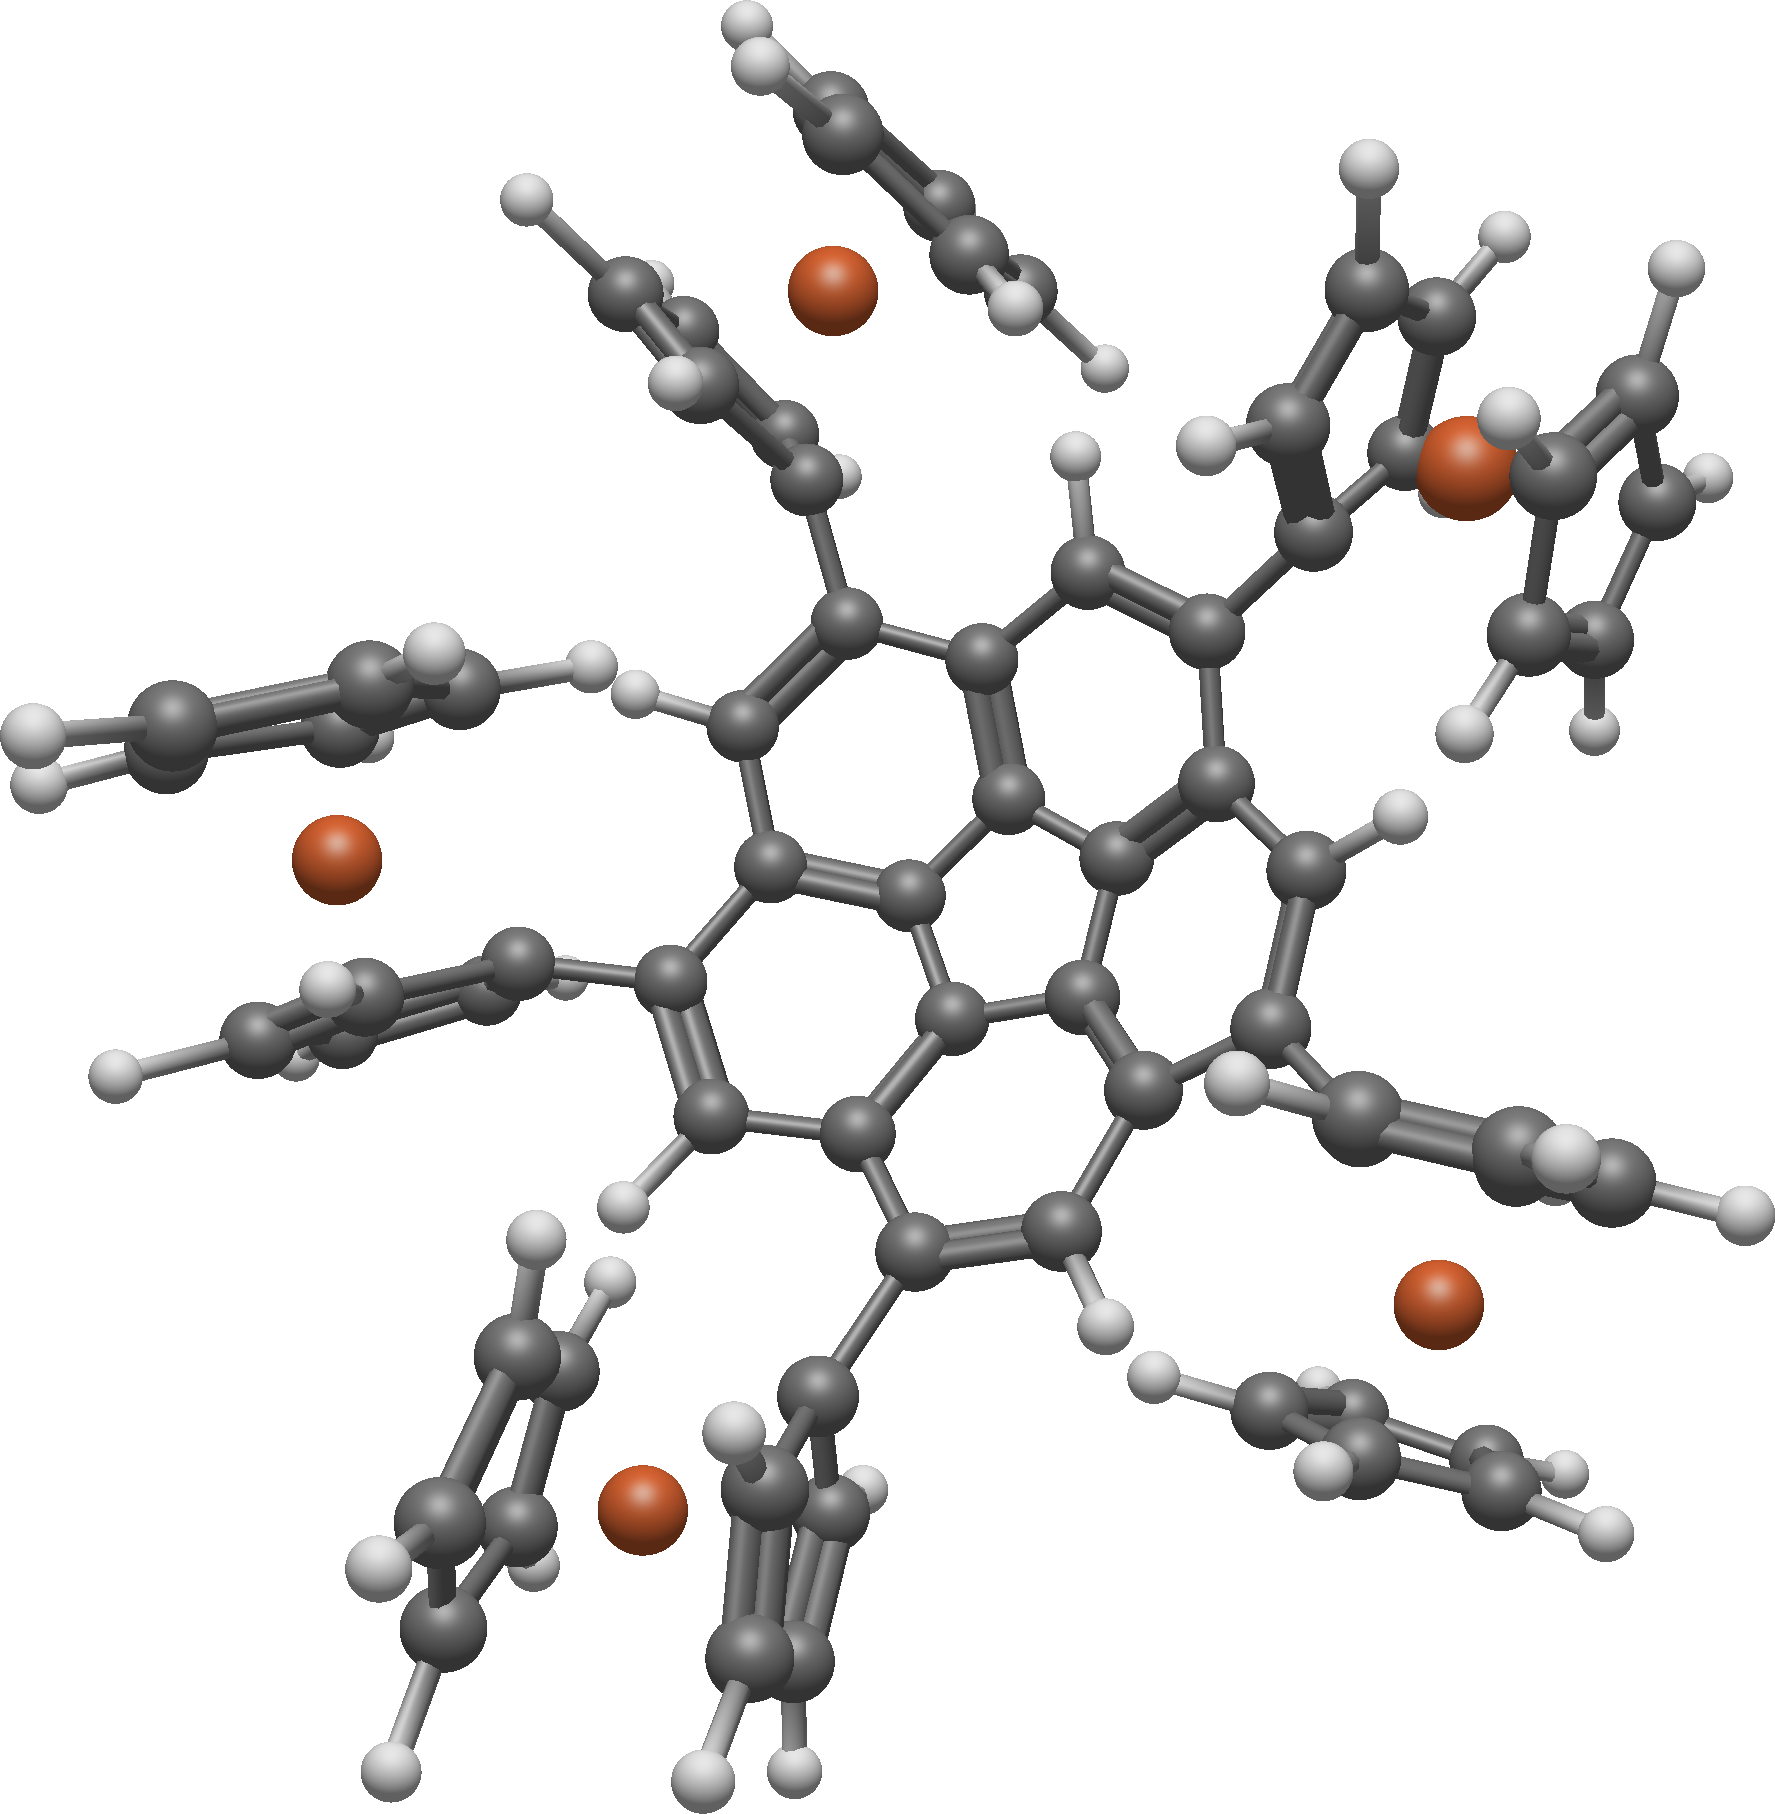
\includegraphics[width=\linewidth]{figures/fercor.png}
        \caption{Structure of 1,3,5,7,9-penta(ferrocenyl)corannulene (\ch{C20H5(C5H5FeC5H4)5}), a molecule with $C_5$ symmetry. The ``concave up'' side of the corannulene bowl structure is facing the reader. Original artwork based on a skeletal structure provided by Topolinski et al. \cite{topolinski}}
        \label{fig:fercor}
    \end{figure}

    Likewise, not every point group with threefold symmetry has character values in $\mathbb{Z}$. The point group $C_3$ is a counterexample. This is an abelian point group, and it contains no mirror planes and no $C_2$ axes perpendicular to the principal $C_3$ axis. Its irreducible representations are one-dimensional, so the characters are cube roots of unity. That is, the characters lie in $\mathbb{Q}(\zeta_3)$, not $\mathbb{Z}$. The character table for $C_3$ is shown in Table \ref{tab:c3}. As with the point group $C_5$, molecules belonging to the point group $C_3$ are uncommon. One molecule belonging to the point group $C_3$ is triphenylphosphine (\ch{P(C6H5)3}). This molecule consists of a phosphorus atom bonded to three phenyl functional groups (six carbon aromatic rings). The lone pair on the central phosphorus atom gives the molecule trigonal pyramidal geometry, similar to ammonia. The skeletal structure of this molecule is shown in Figure \ref{fig:pph3}. \cite{miessler2014}

    \begin{table}[ht]
        \centering
        \renewcommand{\arraystretch}{1.5}
        \begin{tabular}{c|ccccc}
            $C_{5}$ & $E$ & $C_5$ & $C_5^2$ & $C_5^3$ & $C_5^4$\\
            \hline
            $A$~~~~ & $1$ & $1$ & $1$ & $1$ & $1$\\
            \multirow{2}{*}{$E_1$~\Bigg\{} & $1$ & $\varepsilon$ & $\varepsilon^2$ & $\overline{\varepsilon^2}$ & $\overline{\varepsilon}$\\
            & $1$ & $\overline{\varepsilon}$ & $\overline{\varepsilon^2}$ & $\varepsilon^2$ & $\varepsilon$\\
            \multirow{2}{*}{$E_2$~\Bigg\{} & $1$ & $\varepsilon^2$ & $\overline{\varepsilon}$ & $\varepsilon$ & $\overline{\varepsilon^2}$\\
            & $1$ & $\overline{\varepsilon^2}$ & $\varepsilon$ & $\overline{\varepsilon}$ & $\varepsilon^2$
        \end{tabular}
        \caption{The character table of the point group $C_5$. Here, $\varepsilon=e^{2\pi i/5}$. Conjugate pairs of characters are grouped together as the irreps labeled $E_1$ and $E_2$, following the convention in chemistry. \cite{miessler2014}}
        \label{tab:c5}
    \end{table}

    \begin{table}[ht]
        \centering
        \renewcommand{\arraystretch}{1.5}
        \begin{tabular}{c|ccc}
            $C_{3}$ & $E$ & $C_3$ & $C_3^2$\\
            \hline
            $A$~~~~ & $1$ & $1$ & $1$\\
            \multirow{2}{*}{$E_1$~\Bigg\{} & $1$ & $\varepsilon$ & $\overline{\varepsilon}$\\
            & $1$ & $\overline{\varepsilon}$ & $\varepsilon$
        \end{tabular}
        \caption{The character table of the point group $C_3$. Here, $\varepsilon=e^{2\pi i/3}$. The conjugate pair of characters is grouped together as the irrep labeled $E_1$, following the convention in chemistry. \cite{miessler2014}}
        \label{tab:c3}
    \end{table}

    \begin{figure}[H]
        \centering
        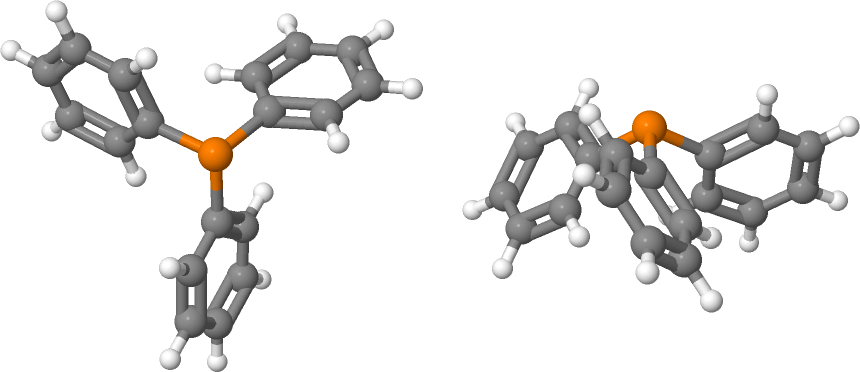
\includegraphics[width=\linewidth]{figures/pph3.png}
        \caption{Structure of triphenylphosphine (\ch{P(C6H5)3}), a molecule with $C_3$ symmetry, shown from two perspectives.}
        \label{fig:pph3}
    \end{figure}
    
    \section{Conclusion}

    In this paper, we studied molecular symmetry from both a chemical and an algebraic point of view. Beginning with the point groups $C_{2v}$ and $C_{3v}$, we described their symmetry operations, constructed matrix representations, and used characters to decompose these representations into irreducible components. By analyzing the eigenvalues and minimal polynomials of the representation matrices, we showed that the eigenvalues of symmetry operations are roots of unity and therefore lie in cyclotomic fields. this provided a number-theoretic framework for understanding what character values take the forms that they do.

    We then used Galois actions to explain an important distinction among point groups. In groups such as $C_{3v}$, although the eigenvalues lie in cyclotomic fields, the associated character values align pairs of eigenvalues in such a way that the characters lie in $\mathbb{Z}$. In contrast, for point groups with fivefold symmetry, the same framework leads to non-integer character values lying in the real subfield $\mathbb{Q}(\sqrt{5})\subset\mathbb{Q}(\zeta_5)$. Thus, the structure of character tables is governed not only by representation theory, but also by the arithmetic of cyclotomic fields and the action of their Galois groups.

    More broadly, this work shows that molecular symmetry is not only geometrically visible, but also algebraically rich. The same symmetry operations that describe the shapes of molecules also determine representation-theoretic and number-theoretic patterns in their character tables. What begins with rotations and reflections in familiar molecules ultimately leads to cyclotomic fields, irreducible representations, and Galois symmetry. This reveals molecular point groups as a setting in which chemistry and algebra are deeply intertwined.

    \section{Future directions}

    This paper has analyzed the algebraic structure of a selection of point groups, including $C_{2v}$, $C_{3v}$, certain groups with fivefold symmetry, and a couple of abelian symmetry groups. A deeper analysis could expand the scope into other point groups, such as those of high symmetry (such as $T_d$, $O_h$, and $I_h$), those with other orders (such as $C_{4v}$, $D_{6h}$, and $D_{8h}$), and additional groups such as $D_n$ or $S_{2n}$, to determine how the associated character fields vary systematically with the structure of the point group.
    
    Another area of consideration is to analyze linear point groups such as $C_{\infty v}$ and $D_{\infty h}$. Here, the finite group framework is replaced by continuous symmetry groups related to the Lie groups $SO(2)$ and $O(2)$. In this setting, characters are no longer discrete values in cyclotomic fields, but rather continuous functions such as $2\cos(n\theta)$. This suggests a broader perspective in which molecular symmetry connects naturally to the representation of Lie groups and Fourier analysis.

    The examples in this paper show that character values can lie in $\mathbb{Q}$, in quadratic fields such as $\mathbb{Q}(\sqrt{5})$, or in cyclotomic fields. One direction is to determine, for different point groups, the smallest field that contains all of their character values and to look for patterns across families of groups. In addition, the appearance of non-integer character values is closely related to the structure of the irreducible representations involved. It would be interesting to explore systematically how the dimension and type of irreducible representations influence whether character values are rational or irrational. Furthermore, one could study how Galois actions organize eigenvalues into orbits, and how these orbits determine the resulting character values.

    The focus of this work on geometric (Cartesian) representations, along with permutation-type representations arising from atomic positions. A natural extension would be to investigate whether the same cyclotomic and Galois-theoreic structure appears in other representations commonly used in chemistry, such as vibrational representations or those arising in molecular orbital theory, where symmetry-adapted linear combinations (SALCs) play a central role.

    Finally, examples such as corannulene and ferrocene show that molecular symmetry can change due to geometric or electronic effects. One could explore how the associated character values and their underlying number fields change when the point group of a molecule changes.
    
    \section{Acknowledgments}

    I would like to express my most sincere gratitude to my advisor, Dr.\ Lilit Martirosyan, for her guidance, encouragement, and insightful feedback throughout this project.

    I am also grateful to Dr.\ Sean English for his engaging teaching and for continually challenging me to think more deeply about mathematics, and to Dr.\ Russell Herman for his instruction and influence on my mathematical curiosity and development.

    I would like to thank Dr.\ Nicholas Chiappini for carefully reviewing the chemistry in this paper, as well as Dr.\ Erik Slivken for this thoughtful input. I am also thankful to Dr.\ Dijana Jakelic for the opportunity to present my work and offer constructive feedback.

    I would also like to acknowledge Dr.\ Thomas Coombs, Dr.\ Bart Jones, and Dr.\ Robert Hancock, whose teaching helped me develop my knowledge and interest of chemistry.

    I am grateful to my classmates for their encouragement and support throughout this process. Finally, I would like to thank my wife, Samantha, and my pets for their unwavering love, support, and patience.   

    \printbibliography[heading=bibnumbered]
\end{document}